\documentclass[final,fmstyle]{util/ucathesis}
%\documentclass[draft, fmstyle]{util/ucathesis}

% La opción 'final' muestra los graficos, para generar una version sin los graficos utiliza la opcion 'draft'

% paquetes recomendados
%\usepackage[chapter]{theorems}
%\usepackage{symbols}
%\usepackage{url}
\usepackage{amsmath,amsthm}
\usepackage[utf8]{inputenc}
\usepackage[spanish]{babel}
\usepackage{csquotes}
\usepackage[style=numeric,sorting=none,backend=biber]{biblatex}
\usepackage{tabularx}		
\usepackage{pdflscape}
\usepackage{listings}
% para la lista de símbolos
%\usepackage{subfigure} %conflicto con subcaption
\usepackage{array}
\usepackage{perpage}
\usepackage{backnaur}
\usepackage{enumerate}
\usepackage{multirow}
\usepackage{adjustbox}
\usepackage{float}
\usepackage{pifont}

%%agregados
%Hipervinculos
\usepackage{hyperref}
\usepackage{subcaption}
\usepackage{amssymb}
\usepackage[table,xcdraw]{xcolor}
\usepackage{longtable}
\usepackage{tikz}
\usepackage{pgfplots}

%tabla
\usepackage{arydshln}

%Colores
\definecolor{color1}{HTML}{4F81BD}
\definecolor{color2}{HTML}{9BBB59}

\MakePerPage{footnote}
\addbibresource{referencias.bib}


%se importan las configuraciones customizadas realizadas.
%%%
%%% Conjuto de funciones utilitarias
%%% autor: Maximiliano Báez
%%% fecha: 25/08/2014
%%%

\usepackage{tablefootnote} %para utilizar \footnote{}
\usepackage{amssymb}
\renewcommand{\thefootnote}{\arabic{footnote}}

%%Para la construcción de la lista de simbolos
% Macro for 'List of Symbols', 'List of Notations' etc...
\def\listofsymbols{
    \newpage
\chapter*{Lista de Acrónimos\hfill}
\addcontentsline{toc}{chapter}{Lista de Acrónimos}
\begin{tabbing}
% YOU NEED TO ADD THE FIRST ONE MANUALLY TO ADJUST THE TABBING AND SPACES
%$x$~~~~~~~~~~\=\parbox{5in}{X\dotfill \pageref{symbol:x}}\\
%ADD THE REST OF SYMBOLS WITH THE HELP OF MACRO

%% se añaden nuevos simbolos con el macro \newsymbol y se hace referecnia
% al simbolo utilizando \addsymbol{symbol:LABEL}


\textbf{OCDS} Open Contracting Data Stantard\\
\textbf{W3C} World Wide Web Consortium\\
\textbf{OWL} Ontology Web Language\\
\textbf{CSV} Comma Separated Value\\
\textbf{JSON} Javascript Object Notation\\
\textbf{JSON-LD} Javascript Object Notation - Linked Data\\
\textbf{XML} Extended Markup Language\\
\textbf{URI} Unified Resource Identifier\\
\textbf{DL} Description Logic\\
\textbf{LOV} Linked Open Vocabularies\\
\textbf{LOD} Linked Open Data\\
\textbf{RDF} Resource Description Framework\\
\textbf{RDFS} Resource Description Framework Schema\\
\textbf{OCP} Open Contractic Partnership\\
\textbf{TED} Tender Electronic Daily\\
\textbf{DNCP} Dirección Nacional de Contrataciones Públicas\\
\textbf{ODP} Ontology Design Pattern\\
\textbf{VOWL} Visual Notation for OWL\\
\textbf{FOAF} Friend Of a Friend\\
\textbf{ORSD} Especificación de Requerimientos Ontológicos\\
\textbf{NOR} Not Ontologic Resource\\
\textbf{PCO} Public Contract Ontology\\
\textbf{API} Application Programming Interface\\



\end{tabbing}
    \clearpage{}
}
\def\newsymbol #1: #2#3{$#1$ \> \parbox{5in}{#2 \dotfill \pageref{#3}}\\}
\def\addsymbol#1{\label{#1}}

% Para las imagenes en grilla
% custom commands
\newcommand{\foreign}[1]{{\it #1}}
\DeclareMathOperator*{\argmax}{arg\,max}
%\algsetup{}
% \algsetup{
%     indent=4em,
%     linenosize=\small,
%     linenodelimiter=.
% }

\usepackage{amsmath}

%% se utilizan para referenciar figuras, tablas, secciones y algoritmos
\newcommand{\figref}[1]{Figura \ref{#1}}
\newcommand{\tabref}[1]{Tabla \ref{#1}}
\newcommand{\chapref}[1]{Capítulo \ref{#1}}
\newcommand{\secref}[1]{Sección \ref{#1}}
\newcommand{\algref}[1]{Algoritmo \ref{#1}}
\newcommand{\apenref}[1]{Apéndice \ref{#1}}


%Traducción al español del paquete algorithmic%
% \floatname{algorithm}{Algoritmo}
% \renewcommand{\listalgorithmname}{Lista de algoritmos}
% \renewcommand{\algorithmicrequire}{\textbf{Entrada:}}
% \renewcommand{\algorithmicensure}{\textbf{Salida:}}
% \renewcommand{\algorithmicend}{\textbf{fin}}
% \renewcommand{\algorithmicif}{\textbf{si}}
% \renewcommand{\algorithmicthen}{\textbf{entonces}}
% \renewcommand{\algorithmicelse}{\textbf{si no}}
% \renewcommand{\algorithmicelsif}{\algorithmicelse,\ \algorithmicif}
% \renewcommand{\algorithmicendif}{\algorithmicend\ \algorithmicif}
% \renewcommand{\algorithmicfor}{\textbf{para}}
% \renewcommand{\algorithmicforall}{\textbf{para todo}}
% \renewcommand{\algorithmicdo}{\textbf{hacer}}
% \renewcommand{\algorithmicendfor}{\algorithmicend\ \algorithmicfor}
% \renewcommand{\algorithmicwhile}{\textbf{mientras}}
% \renewcommand{\algorithmicendwhile}{\algorithmicend\ \algorithmicwhile}
% \renewcommand{\algorithmicloop}{\textbf{repetir}}
% \renewcommand{\algorithmicendloop}{\algorithmicend\ \algorithmicloop}
% \renewcommand{\algorithmicrepeat}{\textbf{repetir}}
% \renewcommand{\algorithmicuntil}{\textbf{hasta que}}
% \renewcommand{\algorithmicprint}{\textbf{imprimir}}
% \renewcommand{\algorithmicreturn}{\textbf{retorna}}
% \renewcommand{\algorithmictrue}{\textbf{cierto }}
% \renewcommand{\algorithmicfalse}{\textbf{falso }}
% \renewcommand{\algorithmiccomment}{\textbf{comentario: }}

%Traducción al español del paquete algorithm2c%

\SetKwInput{KwIn}{Entrada}%
\SetKwInput{KwOut}{Salida}%
\SetKwInput{KwData}{Datos}%
\SetKwInput{KwResult}{Resultado}%
\SetKw{KwTo}{a}%
\SetKw{KwRet}{devolver}%
\SetKw{Return}{devolver}%
\SetKwBlock{Begin}{inicio}{fin}%
\SetKwRepeat{Repeat}{repetir}{hasta que}%
%
\SetKwIF{If}{ElseIf}{Else}{si}{entonces}{sin\'o, si}{en otro caso}{fin si}
\SetKwSwitch{Switch}{Case}{Other}{seleccionar}{hacer}{caso}{sin\'o}{fin caso}{fin seleccionar}
\SetKwFor{For}{per}{fai}{fine per}%
\SetKwFor{ForPar}{par}{hacer in paralelo}{fin para}%
\SetKwFor{ForEach}{para cada}{hacer}{fin para cada}
\SetKwFor{ForAll}{para todo}{hacer}{fin para todo}
\SetKwFor{While}{mientras}{hacer}{fin mientras}



\addtocontents{loa}{\protect\thispagestyle{empty}}

% add this to align the list of algorithms
\makeatletter
  \renewcommand*{\listof}[2]{%
    \@ifundefined{ext@#1}{\float@error{#1}}{%
      \@namedef{l@#1}{\@dottedtocline{1}{2em}{1.3em}}% line of the list (change from 1em to the desired value)
      \float@listhead{#2}%
      \begingroup\setlength{\parskip}{\z@}%
        \@starttoc{\@nameuse{ext@#1}}%
      \endgroup}}
  \renewcommand*\l@algocf{\@dottedtocline{1}{1em}{2.3em}}% line of the list (change from 1em to the desired value)
\makeatother



% \setcounter{tocdepth}{3}

%Datos de la tesis
\title{Mejora de la interoperabilidad semántica de los datos utilizando ontologías para el dominio de Contrataciones Publicas del Paraguay}
\author{Rodrigo Valdez y Camilo Báez}
\degree{Informática}

\advisors{Orientadores:}{Phd. Gustavo Gimenez Lugo
\\Phd. Juan Pane}

\logosource{./figuras/politecnica_logo.jpg}
\institution{Universidad Nacional de Asunción}
\faculty{Facultad Politécnica}
\address{San Lorenzo - Paraguay}

%\newtheorem{definicion}{Definicin}
%\numberwithin{algorithm}{chapter}

% \logosource{./graphics/logo.jpg}
% \institution{Universidad Nacional de Asunci\'{o}n}
% \faculty{Facultad Polit\'{e}cnica}
% \address{San Lorenzo - Paraguay}

\usepackage{glossaries}
\usepackage{etoolbox}
\usepackage[xindy]{imakeidx}

\newtoks\customtok


\renewcommand*{\newacronymhook}{%
 \edef\dosetkeys{\noexpand\setkeys{glossentry}{user1={},\the\glskeylisttok}}%
 \dosetkeys
 \ifcsempty{@glo@useri}%
 {%
   \expandafter\customtok\expandafter{\the\glsshorttok}%
 }%
 {%
   \edef\custom{\the\glsshorttok, \csexpandonce{@glo@useri}}%
   \expandafter\customtok\expandafter{\custom}%
 }%
}

\newcommand*{\custompostdesc}[1]{%
  \ifcsempty{glo@#1@useri}{}{ (\glsentryuseri{#1})}%
}

\renewcommand*{\CustomAcronymFields}{%
  user1={},%
  name={\the\glsshorttok},%
  description={\the\glslongtok\noexpand\custompostdesc{\the\glslabeltok}},%
  first={\the\glslongtok\space(\the\customtok)},%
  firstplural={\the\glslongtok\noexpand\acrpluralsuffix
    \space (\the\customtok)}%
  text={\the\glsshorttok},%
  plural={\the\glsshorttok\noexpand\acrpluralsuffix}%
}

\SetCustomStyle

\makeglossaries
\makeindex

\pgfplotsset{compat=1.12}

\begin{document}

\maketitle     % esto hace las portadas

% Agradecimientos y dedicatoria
\begin{dedicatoria} 

Dedicamos este trabajo a nuestras familias y en especial, a quiénes formaron parte de este proceso \dots

\end{dedicatoria}
\begin{thankspage} 
A nuestras familias y amigos que nos dieron su apoyo incondicional en este proceso de formación.

A nuestros compañeros de facultad que vivieron con nosotros la lucha constante de autosuperación para ser profesionales dignos que ayuden a construir este país.

A la Facultad Politécnica que fue nuestro segundo hogar durante nuestros años de estudio.

Al querido Profesor Gustavo Gimenez Lugo y todos los profesores que dedicaron su tiempo en transmitirnos sus conocimientos sin recelos.

\end{thankspage}
\begin{resumen}


    
\textbf{Palabras clave:} Web Semántica,  Ontologías, Contrataciones Públicas, Open Contracting, OWL, Sparql.
\end{resumen}



\begin{resuingles}
Chagas disease is a tropical parasitic disease caused by the protist Trypanosoma cruzi, it is considered by the World Health Organization as a neglected tropical disease. Neglected tropical diseases are those that affect a high amount of the population, mostly on third world countries, and have an expensive, inefficient or inexistent treatment. The first step in determining the effectiveness of new antichagasic drugs that help reduce the costs of treating the disease is the counting of the intracellular parasitic form (amastigote) under a microscope.
The watershed transform is an image segmentation algorithm.
Image segmentation is the process of partitioning a digital image into its constituent regions. Said segmentation is an important process to perform a count of Trypanosoma cruzi amastigotes and thus determine the efficacy of new antichagasic drugs.The watershed algorithm has been used in to solve the segmentation problem, most often in grayscale images. Grayscale images may lose important information for segmentation, this is because it only uses the intensity of the colors. The color images give more information, but implementing the color watershed transform is not trivial. The implementation of the watershed transform by flooding in color images proposed by Meyer, requires an order between the pixels to perform the segmentation. This work extends the watershed algorithm by flooding for color images using the CIELab color space for the segmentation of Trypanosoma Cruzi Amastigotes in microscopic cell images. It uses the Euclidean distance to a reference color for the ordering of the pixels. The proposed method was compared with the implementation of the watershed transform in different color spaces and using different pixel ordering methods. The CIELab color space using the distance to the median of the colors presented the best results with an accuracy of 91 \%. The CIELab color space obtained better results regardless of the reference color used in relation to the methods in the different color spaces and grayscale images. The proposed segmentation method can be used to identify Trypanosoma cruzi amastigotes, and in this way can count and collect statistics necessary to produce new drugs for Chagas disease.

\end{resuingles}




% los siguientes comandos producen 'indices.


% Tabla de contenidos
\tableofcontents
% Lista de figuras
\listoffigures
% Lista de tablas
\listoftables
% Lista de algoritmos
\listofalgorithms
\printglossary[type=\acronymtype,title=Lista de Siglas]
\addcontentsline{toc}{chapter}{Lista de Siglas}
\newacronym{rgb}{RGB}{Red Green Blue}
\newacronym{hsi}{HSI}{Hue Saturation Intensity}
\newacronym{cie}{CIE}{Commission Internationale de l’Eclairage}
\newacronym{oms}{OMS}{Organización Mundial de la Salud}
\newacronym{cielab}{CIELab}{Espacio de Color presentado por la CIE}

% Lista de simbolos
\listofsymbols


\mainmatter  % inician los capitulos de la tesis

% incluye aqui los capitulos (un archivo .tex por capitulo)
% los capitulos
%!TEX root = ../main.tex
\chapter{Introducción}
\label{chap:introduccion}
Según el reporte de la Open Contracting Partnership (OCP), los Gobiernos de todo el mundo gastan un estimado de 9.5 billones de dólares anualmente mediante contratos. Sin embargo, en la mayoría de los países, la información sobre estos contratos no está disponible para el escrutinio público, haciendo al proceso de contratación vulnerable a la corrupción y la mala gestión. Además, los países que sí lo hacen, no proveen un contexto apropiado para entender, reutilizar e integrar dichos datos con otros.

Debido a la creciente importancia de publicar los datos de contrataciones públicas  los Estados crean portales de datos con el fin de transparentar los procesos y establecer mecanismos para que la ciudadanía, empresas y organizaciones puedan ejercer un rol de contralores y a la vez facilitar a los entes gubernamentales a contratar bienes y servicios. Este es el caso del portal Tender Electronic Daily (TED) en la Unión Europea, República Checa, y la Municipalidad de Palmares en Costa Rica. En Paraguay, estos datos pueden ser obtenidos desde el Portal de Datos Abiertos de la Dirección Nacional de Contrataciones Públicas (DNCP).

Según Svátek, los datos de contrataciones públicas son importantes dentro de la Web Semántica porque unifican dos esferas muy diferentes como son: las necesidades públicas por un lado y la oferta de productos y servicios del sector privado por el otro; este escenario es idóneo para la utilización de modelos de datos, metodologías y fuentes de información publicadas de forma independiente. Además, la gran cantidad de datos de contrataciones públicas da lugar para aplicar diversos métodos de análisis de datos que van desde estadísticas agregadas en forma de barras hasta análisis más exhaustivos de minería de datos.
Este trabajo nace con la intención de crear una ontología capaz de mejorar la accesibilidad a la información pública, y que dicha información sea comprensible por máquinas con el fin de brindar mayor desarrollo y transparencia al proceso de contrataciones públicas.



\section{Justificación}

Debido a la gran cantidad de datos disponibles en internet, la integración entre sistemas de información heterogéneos que disponibilizan estos datos se vuelve un problema complejo de resolver para poder quitar provecho de los mismos. 

Este desafío puede ser abordado a través de tecnologías de la Semantic Web, en ella se integran estándares y herramientas necesarias para la disponibilización de recursos en la web de manera a que sean entendibles por máquinas y a la vez haciendo posible la integración de recursos de diferentes fuentes. En este aspecto, las ontologías proveen una descripción de los datos que no depende de un contexto en particular y puede ser entendido tanto por sistemas de información como por personas, logrando así la interoperabilidad semántica.

El problema computacional que se quiere resolver es la interoperabilidad sintáctica y semántica de datos de un dominio de conocimiento en particular con datos de distintas fuentes de publicación y de distintos dominios de conocimientos. El trabajo pretende modelar una ontología para brindar una capa de semántica formal a un estándar de datos abiertos para la publicación de datos estructurados llamado Open Contracting Data Standard (OCDS), aplicado a datos de la DNCP utilizando metodologías y herramientas para el desarrollo de ontologías. 


\section{Objetivo General del Proyecto}

El objetivo general es verificar experimentalmente la expresividad asociada a la interoperabilidad semántica establecida por una ontologías desarrollada con base en un protocolo de intercambio de datos.


\section{Objetivos Específicos}
\label{objetivos especiicos}

\begin{enumerate}
    \item \label{obj:1}  Identificar y comparar las bases representación de conocimientos asociado al dominio de Contrataciones Públicas.
    \item \label{obj:2}  Describir el proceso de modelado de una ontologia utilizando una base de representacion de conocimiento de dominio.
    \item \label{obj:3}  Modelar un sistema de extracción y consultas de datos del dominio Contrataciones Públicas con capacidad de integración semántica.
    \item \label{obj:4}  Mostrar el uso de la ontologia con datos de Contrataciones Publicas del Paraguay.
\end{enumerate}


\section{Contribuciones}
\label{Contribuciones}
\begin{itemize}
\item Sistema de extracción y manipulación de datos de Procesos Licitatorios con capacidad de integracion con fuentes externas de datos como Wikidata.
\item Descripción del proceso de modelado de una Ontología, reutilizando de un recurso no-ontológico basado en JSON-SCHEMA.
\item Una Ontología basada en el Open Contracting Data Standard.
\item Descripciones experimentales de la pragmática de incorporación, uso y reuso de ontologías para aumentar la interoperabilidad en los datos publicados.

\end{itemize}
 

\section{Estructura del documento}
El trabajo está estructurado de la siguiente manera; en  en el  Capítulo \ref{chap:Marco Teorico}  trataremos el marco teórico del trabajo abordando los temas de la web semántica, las ontologías, sus metodologías y herramientas. En el Capítulo \ref{chap:Desarrollo de la Ontologia} se mostrará el proceso del modelado de la ontología, en el Capítulo \ref{chap:Implementación de la Ontologia} se implementará el entorno tecnológico de experimentación para luego en el Capítulo  \ref{chap:Contexto experimental} mostrar las pruebas realizadas a los datos que utilizan la ontología desarrollada. En el Capítulo \ref{chap:conclusiones} se evaluará el cumplimiento de los objetivos propuestos, las conclusiones finales y futuros trabajos que pudieran abordarse. Al final de este documento  se  incluyen las referencias bibliográficas utilizadas para su elaboración y el anexo que provee información complementaria al trabajo.



%!TEX root = ../main.tex
\chapter{Marco Teórico}
\label{chap:Marco Teorico}

En esta capítulo abordaremos los conceptos teóricos necesarios para la elaboración de este trabajo. Primeramente veremos los conceptos de Datos Abiertos. Se abordara los estándares y tecnologías a los cuales se definen dentro de la Web Semántica y la interoperabilidad semántica. Por último se abordará la teoría de construcción de ontologías, su aplicación dentro de la web semántica, así como también los formatos de serialización y herramientas para consultar datos.


\section{Datos Abiertos}

 Los datos abiertos son datos que pueden ser utilizados, reutilizados y redistribuidos libremente por cualquier persona, y que se encuentran sujetos, cuando más, al requerimiento de atribución y de compartirse de la misma manera en que aparecen\cite{bauer2011linked} \cite{OpenDataHandBook:online}.
 

A través de los datos abiertos son importantes porque gracias a ellos se puede lograr la interoperabilidad, que significa que diversos sistemas y organizaciones puedan trabajar juntos e integrar diferentes conjuntos de datos. Esta habilidad de integrar componentes es esencial para construir sistemas complejos y grandes\cite{OpenDataHandBook:online}.

\subsection{Datos Abiertos Enlazados}

Los datos abiertos enlazados se enfocan en un método de publicación de datos abiertos estructurados para que puedan ser interconectados. Para lograr esto se utilizan las tecnologías como RDF, RDFa, etc. para estructurar los datos, utilizando URIs para identificar los datos individualmente. Tim Berners Lee define un modelo de 5 estrella \cite{Linke48:online} para clasificar e identificar el grado de publicación de datos abiertos.

\begin{table}[!htb]
\centering
\caption{Modelo de publicación de 5 estrellas\cite{Linke48:online}.}
\label{modelo-5-estrellas}
\resizebox{15cm}{!} {
\begin{tabular}{|c|l|}
\hline
\ding{72} & La información está disponible en la web (en cualquier formato) bajo una licencia abierta \\ \hline
\ding{72} \ding{72} & La información está disponible como dato estructurado (Ej. Excel en lugar de una imagen de una tabla) \\ \hline
\ding{72} \ding{72} \ding{72} & Son utilizados formatos no-propietarios (Ej. CSV en lugar de Excel) \\ \hline
\ding{72} \ding{72} \ding{72} \ding{72}  & URIs son utilizadas para que se puedan individualizar los datos \\ \hline
\ding{72} \ding{72} \ding{72} \ding{72} \ding{72}  & Los datos son enlazados con otros datos para proveer un contexto \\ \hline
\end{tabular}
}
\end{table}

\section{La Web Semántica}
La Web Semántica consiste en una serie de estándares y tecnologías propuestas por la W3C\cite{Semantic20:online} que promueven el uso de formatos de datos común y además de un protocolo de datos dentro de la web que nos permite compartir y reusar datos -procesables por máquinas- a través de la web. Se puede pensar la Web Semántica como una manera eficiente de representar datos en la web\cite{TimBernersLeee}\cite{Shadbolt:2006}.

El principal problema de los datos en la web es la dificultad de su utilización a gran escala, ya que no siempre se aplican estándares de publicación de datos de manera a que facilite su procesamiento. Por otra parte, los datos enlazados a través de identificadores comunes en la web nos dan la capacidad de consultar datos de distintas fuentes y contestar preguntas complejas pero interpretar el significado de los mismos no resulta una tarea sencilla. Es por eso que las ontologías juegan un rol fundamental en la Web Semántica, ya que gracias a ellas podemos representar conocimiento legible y entendible por máquinas y humanos en la web.

\section{Interoperabilidad Semántica}
\label{section:interoperabilidadsemantica}
La interoperabilidad es la capacidad de dos o más sistemas de compartir y usar la  información. En la interoperabilidad semántica, los sistemas deben poder intercambiar información de tal manera que el significado del dato sea accesible y comprendido correctamente por cualquier sistema (o persona)\cite{Interoperability}\cite{Schulz2013HowOC}. Al contrario, la interoperabilidad sintáctica se preocupa en el intercambio de datos estructurados -a través de un estándar o formato común- a fin de lograr la interoperabilidad.
Para lograr la interoperabilidad semántica hacemos uso de ontologías, las mismas nos permiten representar un modelo de datos que refleja un dominio de conocimiento dado.

\section{Ontologías}
Las ontologías son utilizadas para la representación del conocimiento, logrando así que la información esté representada de forma a que pueda ser interpretada por los computadores y humanos\cite{horrocks2011kr}. En ella se definen los conceptos de un determinado dominio, sus propiedades y relaciones entre los mismos, así también reglas para combinar términos y relaciones que permitan extender el vocabulario.
A continuación se pone a conocimiento algunas definiciones hechas acerca de las ontologías en el ámbito de sistemas de información.

Gruber\cite{gruber1993translation} definió originalmente el concepto de ontología como “Una especificación explícita de una conceptualización”. Borst\cite{borst1997construction} definió una ontología como “Una especificación formal de una conceptualización compartida”. La definición que se eligió en este trabajo es la de Studer\cite{studer1998knowledge}: “Una ontología se define como una especificación formal y explícita de una conceptualización compartida”.  En esta definición, conceptualización se refiere a un modelo abstracto de algún fenómeno del mundo derivado de la identificación de sus conceptos relevantes; explícita se refiere a que los tipos de conceptos y las restricciones usadas sobre ellos se definen explícitamente; formal se refiere a que la ontología debe ser “legible” por una computadora; y compartida refleja que una ontología capta un conocimiento consensual. Guarino\cite{guarino1998formal} también definió como “Un conjunto de axiomas lógicos diseñados para tener en cuenta el significado deseado de un vocabulario”.

Actualmente existen ontologías para diversos dominios de conocimiento. Algunas de las más representativas son: \textit{Simple Knowledge Organization System} (SKOS) \cite{isaac2009skos}, \textit{ Friend of a Friend} (FOAF) \cite{brickley2012foaf}, \textit{Good Relations}, \cite{hepp2008goodrelations}, MGED Ontology \cite{whetzel2006mged} y National Cancer Institute Ontology \cite{golbeck2011national}. Así también existen ontologías que no pertenecen a un dominio específico (de alto nivel) y describen conceptos generales como DOLCE\cite{dolce} \cite{Masolo02thewonderweb}.
La ontología posee varios usos en Ciencias de la Computación, como ser en el ámbito legal, médico, científico y otros, pero ganó mayor popularidad en el ámbito de la Web Semántica. A continuación veremos las ontologías en el caso de uso de la web semántica.


\section{Ontologías en la Web Semántica}
Uno de los principios fundamentales de las ontologías dentro de la web semántica es su reutilización y extensión \cite{Thorsen2015OntologiesIT}, esto significa reutilizar conceptos definidos otras ontologías, siempre y cuando sea posible, mejorando el procesamiento y la integración de datos enlazados. En lugar de duplicar esfuerzos definiendo conceptos y propiedades que ya fueron definidos en otra ontología, se puede referenciar a estos elementos dentro de la nueva ontología. 

Existe una variedad de tipos de ontologías que dependen del nivel de formalidad, razonamiento y la cantidad de restricciones\cite{Giunchiglia2009LightweightO} \cite{Obrst}. En el caso más simple una ontología puede describir una jerarquía de conceptos vinculados por relaciones de subsunción y en casos más sofisticados incluir axiomas para expresar relaciones entre conceptos y restringir la interpretación pretendida.

Las ontologías para la Web Semántica son de tipo ligeras en términos de niveles de formalidad y normalmente pequeñas en tamaño haciéndolas fáciles de manejar y mantener\cite{Thorsen2015OntologiesIT}. El poder de expresión de una ontología en la Web Semántica debe ser adecuado, el lenguaje debe ser tan expresivo como para poder describir conceptos con suficiente detalle, pero no tan expresivo como para perder la capacidad de razonamiento\cite{reasonableSemantic}. Una ontología más formal o expresiva es computacionalmente más costosa, por lo que se debe encontrar un equilibrio entre los dos puntos. En la Figura \ref{img:expresividad complejidad } se puede ver el espectro de ontologías según su expresividad y complejidad computacional, en donde el lenguaje OWL y la Lógica de Descripciones se encuentran dentro de las más expresivas y costosas computacionalmente.
La capacidad de razonamiento es importante para asegurar la calidad de la ontología construida, por ejemplo, en la etapa de diseño puede ser utilizada para probar si existen conceptos contradictorios y derivar nuevas relaciones.

Las formas de representar ontologías en la Web Semántica son diversas en cuanto a lenguajes y formas de serialización, a continuación se presenta algunas de ellas.

    \begin{figure}[ht!]
    \centering
    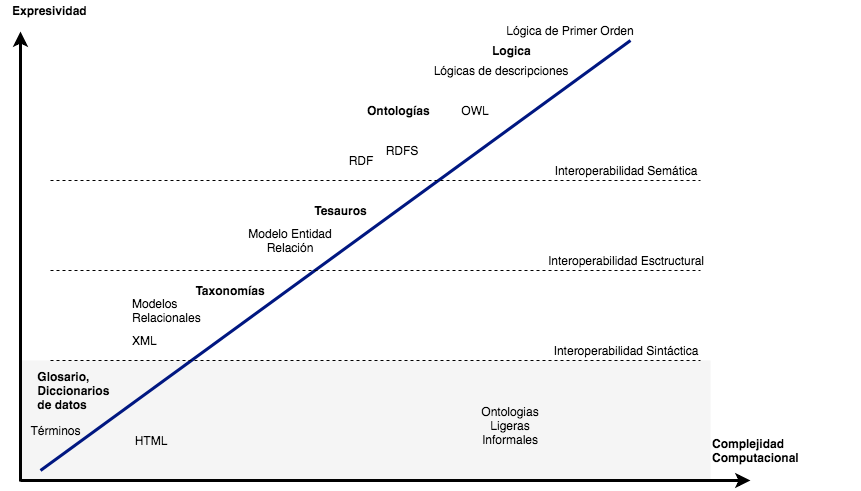
\includegraphics[width=150mm]{figuras/Diagramas-ComplejidadOntologica}
    \caption{Expresividad vs Complejidad. Adaptación de \cite{Giunchiglia2009LightweightO} \cite{Obrst}}
    \label{img:expresividad complejidad }
    \end{figure}



\section{RDF y RDFS (RDF)}

Marco de Descripción de Recursos, RDF por sus siglas \textit{Resource Description Framework}  \cite{rdf}, es un framework para representar información en la Web Semántica. El lenguaje RDF forma parte de la W3C's \textit{Semantic Web Activity} y es recomendado por la W3C \cite{Semantic20:online}. El modelo de datos RDF está diseñado para que sea procesable por computadoras. 

RDF nos permite representar modelos de datos basados en grafos, los cuales son representados en triplas. Las triplas RDF contienen tres componentes:

\begin{itemize}
  \item El sujeto, que puede ser una referencia tipo URI o un \textit{Blank Node}
  \item El predicado, que es una referencia tipo URI
  \item El objeto que puede ser una referencia tipo URI, un literal o un \textit{Blank Node}
\end{itemize}



En la Figura \ref{img:componentes rdf } se expone un grafo de ejemplo en el cual se visualizan estos tres componentes.

    \begin{figure}[ht!]
    \centering
    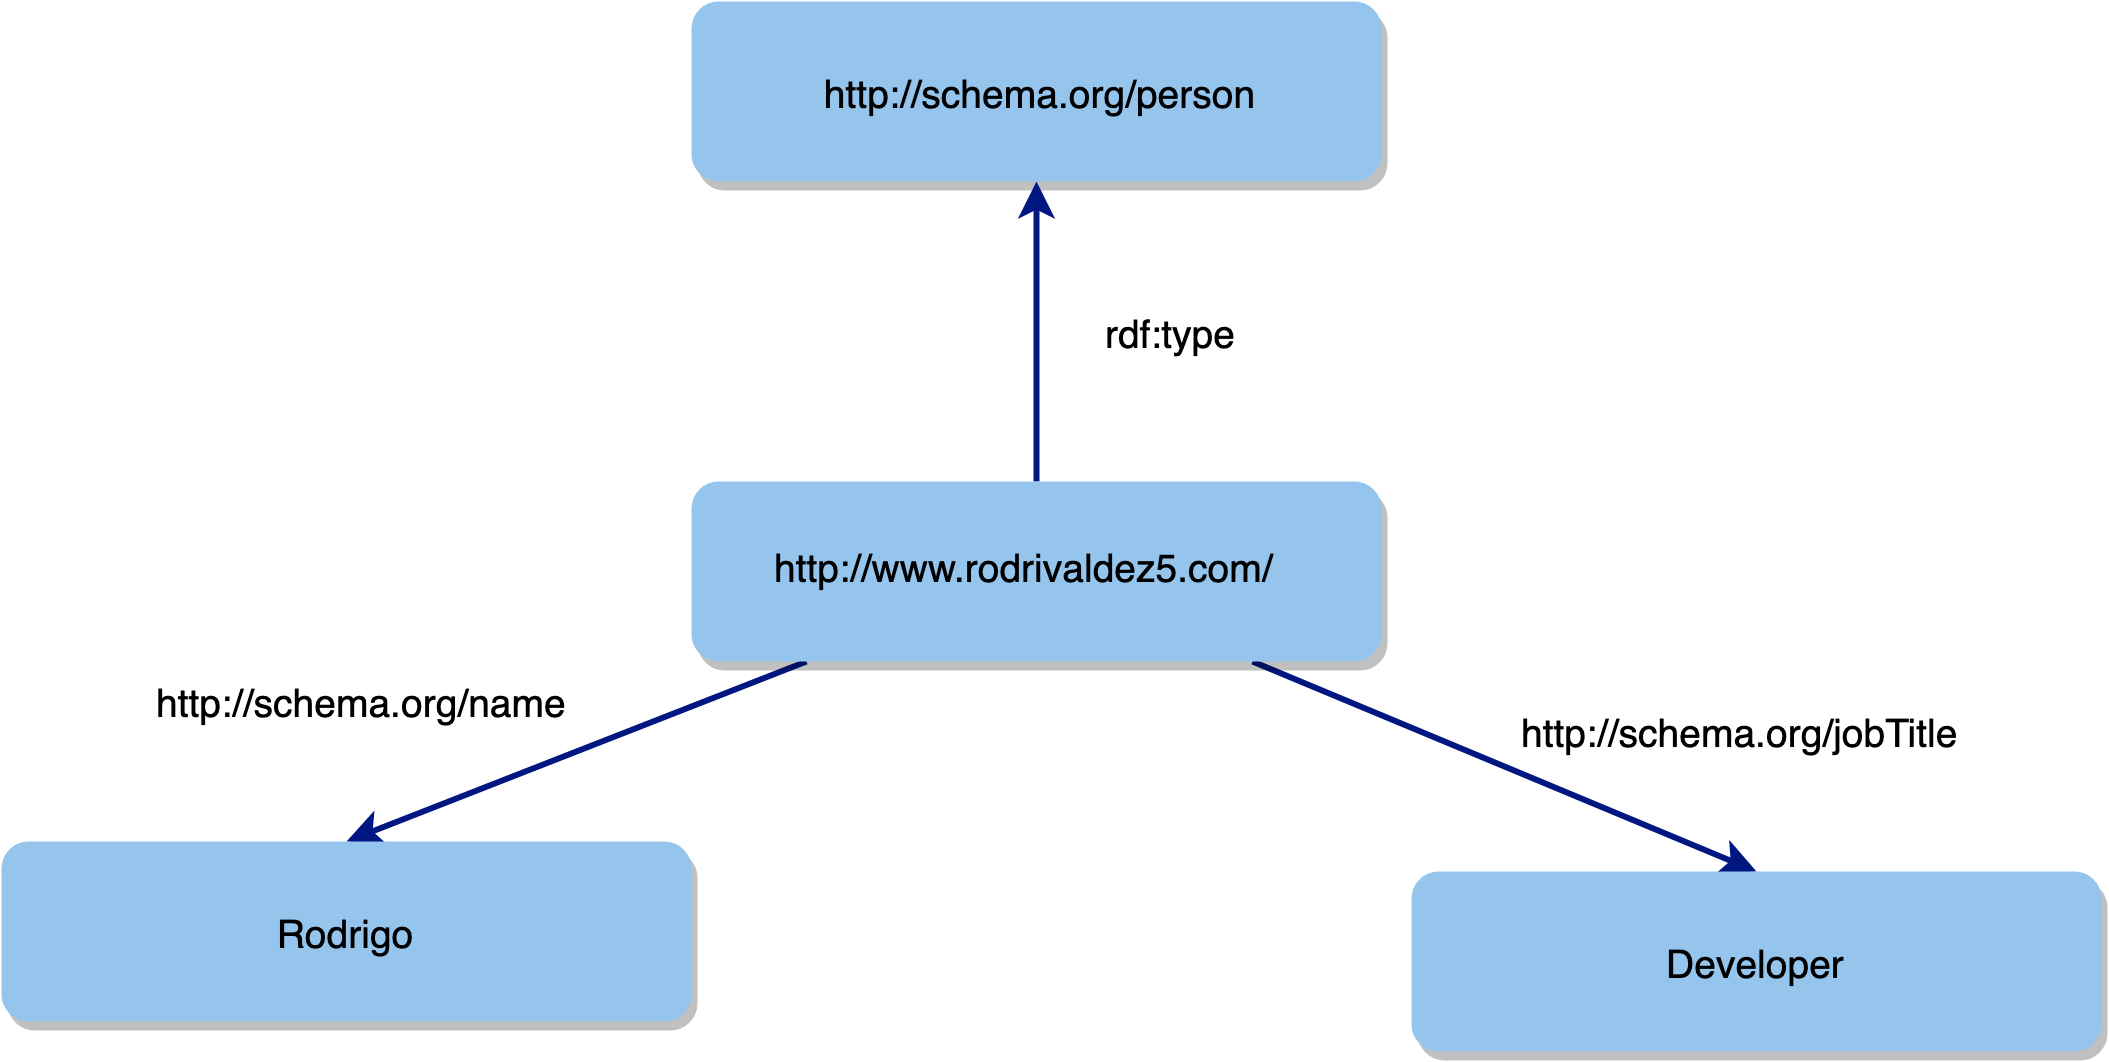
\includegraphics[width=150mm]{figuras/Diagramas-RDFGraph}
    \caption{Componentes RDF}
    \label{img:componentes rdf }
    \end{figure}
    
El sujeto es la fuente de la arista y debe ser un recurso. En RDF, un recurso puede ser cualquier cosa que sea identificable de forma única a través de un URI. Comúnmente este identificador es un URL, que es un caso especial de URI. Sin embargo, los URI son más generales que las URL. En particular, no es requerimiento que un URI se pueda utilizar para localizar un documento en Internet. El objeto de una sentencia es el objetivo de la arista. Al igual que el sujeto, puede ser un recurso identificado por un URI, pero alternativamente puede ser un valor literal como una cadena o un número. Los predicados de una sentencia determinan qué tipo de relación se mantiene entre el sujeto y el objeto. También es identificado por un URI.

Un identificador uniforme de recursos \footnote{https://www.w3.org/wiki/URI} (URI por sus siglas inglés \textit{Uniform Resource Identifier}) es una cadena de caracteres que identifica inequívocamente un recurso en particular. 

Todos los literales tienen una forma léxica que es una cadena \textit{Unicode}. Un literal en un grafo RDF puede presentarse de dos formas:
\begin{itemize}
    \item Los literales simples tienen una forma léxica y, opcionalmente, una etiqueta de idioma normalizada a minúscula. Ej.: “Hola mundo”@es.
    \item Los literales tipados que tienen una forma léxica y una URI de tipo de datos que es una referencia de URI RDF. Ej.: “Hola mundo”\textit{xsd:string}.
\end{itemize}

Un \textit{Blank Node} es un nodo en un documento RDF que representa un recurso para el que no se proporciona un URI o literal y también es llamado recurso anónimo.

RDF es simplemente un representación sictáctica de datos y no provee significado semántico de los mismos. RDF Schema (RDFS) en cambio es una extensión de RDF que nos permite definir un vocabulario para el uso en modelos de datos RDF, permite definir tipo de clases de un recurso y propiedades que un recurso puede tener, esto a través de un vocabulario que incluye\textit{ rdfs:Class, rdf:Property , rdfs:subClassOf, rdfs:subPropertyOf, rdfs:domain, rdfs:range} y otras propiedades de documentación como son \textit{rdfs:label y rdfs:comment}.

La sintaxis de RDF puede escribirse en distintos formatos de serialización: \textit{RDF/XML \footnote{https://www.w3.org/TR/2004/NOTE-owl-parsing-20040121/}, Turtle\footnote{https://www.w3.org/TR/turtle/}, N-Triples \footnote{https://www.w3.org/TR/n-triples/}, N-Quads \footnote{https://www.w3.org/TR/n-quads/} y JSON-LD\footnote{https://json-ld.org/spec/latest/json-ld-rdf/}}.

En el Cuadro \ref{lst:n-quads} se muestra un ejemplo de triplas en formato RDF/N-Quads. \hfill \break

\lstset{language=XML}
    
\noindent\begin{minipage}{\textwidth}
\begin{lstlisting}[captionpos=b, caption=Ejemplo en RDF/N-Quads, label=lst:n-quads,  numbers=left,  numberstyle=\tiny\color{mygray},frame=single]
<http://rodrivaldez5.com/> <http://www.w3.org/2000/01/rdf-schema#type> <http://schema.org/person> .  
<http://www.rodrivaldez5.com/> <http://schema.org/name>"Rodrigo Valdez" .
<http://www.rodrivaldez5.com/> <http://schema.org/telephone>"0981530572" .
<http://www.rodrivaldez5.com/> <http://schema.org/jobTitle>"Developer" .
<http://www.rodrivaldez5.com/> <http://schema.org/image> <http://www.rodrivaldez5.com/images/rodri.png> .
\end{lstlisting}
\end{minipage}

En linea 1, <http://www.rodrivaldez5.com/> es el sujeto, <http://schema.org/image>  es el predicado y <http://www.rodrivaldez5.com/images/rodri.png>  es el objeto, donde el objeto en este caso es una URI. En la línea 2 se puede ver que el objeto se trata de un dato literal de tipo String.  A continuación se presenta JSON-LD, una forma de representación de datos compatible con RDF.

\subsection{Serialización JSON-LD}

JSON, por sus siglas en inglés \textit{JavaScript Object Notation} es un formato de texto utilizado para la representación e intercambio de datos en la web. JSON-LD \cite{JSONLDSy39:online}, donde LD proviene de \textit{Linked Data}, es una extensión de JSON cuya idea es lograr el enlace de datos y agregar una capa de semántica a la web. JSON-LD define un mecanismo para mapear los términos JSON (propiedad y valor) a URIs que poseen información semántica acerca del término. 

Todo objeto JSON-LD es también un objeto JSON. JSON-LD es compatible con RDF ya que se puede representar en triplas, en este caso el nombre de la propiedad (JSON) corresponde al predicado (RDF), el sujeto (RDF) corresponde al objeto (JSON) y el valor de la propiedad (JSON) corresponde al objeto (RDF).

A continuación se plantea un ejemplo de transformación de un documento JSON a JSON-LD 

En el Cuadro \ref{lst:json} se muestra un ejemplo de documento JSON y en el Cuadro \ref{lst:json-ld} se muestra su transformación a JSON-LD.  
\newline

\lstset{language=json}  

\noindent\begin{minipage}{\textwidth}
\begin{lstlisting}[captionpos=b, caption=Ejemplo de un documento JSON, label=lst:json,  numbers=left,  numberstyle=\tiny\color{mygray},frame=single]
{
  "id": "http://www.rodrivaldez5.com/",
  "name": "Rodrigo Valdez",
  "telephone": "0981530572",
  "jobTitle": "Developer",
  "image": "http://www.rodrivaldez5.com/images/rodri.png"
}
\end{lstlisting}
\end{minipage}

\noindent\begin{minipage}{\textwidth}
\begin{lstlisting}[captionpos=b, caption=Ejemplo de un documento JSON-LD, label=lst:json-ld,  numbers=left,  numberstyle=\tiny\color{mygray},frame=single]
{
  "@id": "http://www.rodrivaldez5.com/",
  "@type": "http://schema.org/person",
  "http://schema.org/name": "Rodrigo Valdez",
  "http://schema.org/telephone" : "0981530572",
  "http://schema.org/jobTitle": "Developer",
  "http://schema.org/image":   {"@id":  "http://www.rodrivaldez5.com/images/rodri.png"} 
}
\end{lstlisting}
\end{minipage}
De aquí se puede observar que el principal cambio radica en los nombres de las propiedades, las cuales ahora son URIs válidos, el resultado es equivalente a las triplas RDF del Cuadro \ref{lst:n-quads}

Además JSON-LD permite crear un contexto que contiene el mapeamiento entre el nombre de la propiedad y la URI, dando como resultado el objeto JSON-LD del Cuadro \ref{lst:json-ld-contexto}. \hfill \break

\noindent\begin{minipage}{\textwidth}
\begin{lstlisting}[captionpos=b, caption=Ejemplo de un documento JSON-LD con Contexto, label=lst:json-ld-contexto,  numbers=left,  numberstyle=\tiny\color{mygray},frame=single]
{
  "@context": {
    "name": "http://schema.org/name",  
    "joTitle": "http://schema.org/jobTitle",  
    "telephone": "http://schema.org/telephone",  
    "image": {
      "@id": "http://schema.org/image",  
      "@type": "@id"  
    },
  
  },
  "@id": "http://www.rodrivaldez5.com/",
  "@type": "http://schema.org/person",
  "image": "http://www.rodrivaldez5.com/images/rodri.png",
  "jobTitle": "Developer",
  "name": "Rodrigo Valdez",
  "telephone": "0981530572"
}
\end{lstlisting}
\end{minipage}
El contexto también puede definirse en otro documento diferente y solamente haciendo referencia a éste, quedando el JSON final como se muestra en el Cuadro \ref{lst:json-ld-contexto-referencia}

\noindent\begin{minipage}{\textwidth}
\begin{lstlisting}[captionpos=b, caption=Ejemplo de un documento JSON-LD con Contexto referenciado, label=lst:json-ld-contexto-referencia,  numbers=left,  numberstyle=\tiny\color{mygray},frame=single]
{
  "@context": "http://schema.org/",
  "@id": "http://www.rodrivaldez5.com/",
  "http://schema.org/name": "Rodrigo Valdez",
  "http://schema.org/telephone" : "0981530572",
  "http://schema.org/jobTitle": "Developer",
  "http://schema.org/image":   {"@id": "http://www.rodrivaldez5.com/images/rodri.png"} 
}
\end{lstlisting}
\end{minipage}
El formato JSON es ampliamente utilizado y preferido por los desarrolladores en la web, en comparación con el formato de representación RDF. En la Tabla \ref{prefencia-uso} se muestra la preferencia de uso entre la serialización RDF y JSON-LD en algunas categorías de aplicaciones \cite{rdfjson}.

\begin{table}[!htb]
\footnotesize
\centering
\caption{Preferencias de uso de serialización RDF y JSON-LD \cite{RDFANDJS70:online}}
\label{prefencia-uso}
\resizebox{15cm}{!} {
\begin{tabular}{|l|l|l|}
\hline
 \thead{Categoría de Aplicación} & \thead{RDF o JSON-LD} & \thead{Comentarios}\\\hline
\multicolumn{1}{|m{5cm}|}{Aplicación Web API} & JSON-LD & \multicolumn{1}{m{5cm}|}{La sintaxis está diseñada para integrar fácilmente en sistemas desplegados que ya usan JSON, y proporciona un camino de actualización sin problemas de JSON a JSON-LD}\\\hline
\multicolumn{1}{|m{5cm}|}{Aplicaciones de UI basadas en navegador} & JSON-LD & \multicolumn{1}{m{5cm}|}{La gran cantidad de parsers basados en JSON. Javascript es el lenguaje del navegador}\\\hline
\multicolumn{1}{|m{5cm}|}{Aplicaciones basadas en Inferencia, Razonamiento} & RDF & 
\multicolumn{1}{m{5cm}|}{Gran soporte para razonadores y almacenes de tripletas escalables}\\\hline
\multicolumn{1}{|m{5cm}|}{Herramientas de consultas Expresivas} & RDF & \multicolumn{1}{m{5cm}|}{El estado avanzado de SPARQL 1.1 ayuda a escribir consultas potentes y expresivas}\\ \hline
\end{tabular}
}
\end{table}



\section{\textit{Web Ontology Language }(OWL)}
OWL es un estándar internacional para codificar e intercambiar ontologías y es diseñado para soportar la Web Semántica.

Es el lenguaje de representación de conocimientos recomendado por la W3C y es una extensión de RDFS, dándole mayor expresividad a través de operaciones booleanas (intersección, unión, complemento), restricciones de cardinalidad, cuantificación existencial, etc. El mismo está basado en lenguajes de representación de conocimientos llamados Lógica de Descripciones (DL, por sus siglas en inglés \textit{Description Logic}). DL es un lenguaje formal usado para construir ontologías y permite declarar conocimiento de un dominio específico e incluir reglas de razonamiento para poder procesarlo \cite{kalibatiene2011survey}.

Al estar basado en DL, OWL nos trae consigo las siguientes ventajas
\begin{itemize}
    \item Expresividad: La Lógica de Descripciones nos permite tener expresiones complejas de los conceptos a modelar.
    \item Razonador Automático: La Lógica de Descripciones está basado en lógica formal, eso nos permite desarrollar razonadores capaces de verificar la consistencia de la ontológica e inferir nuevo conocimiento.
\end{itemize}

OWL posee tres sub lenguajes: OWL Lite, OWL DL y OWL Full. Todos permiten describir clases, propiedades e instancias pero difieren uno de otro en el nivel de especificación requerido. OWL Lite está diseñado para usuarios cuyas necesidades de modelado sean simples. OWL DL es lo más cercano a una DL expresiva manteniendo la completitud computacional, esto significa que la ontología es procesable computacionalmente. OWL Full posee mayor expresividad sacrificando la completitud computacional de la ontología. En la Figura \ref{img:subclases owl} se muestra la relación entre los tres sublenguajes.

\begin{figure}[h!]
    \centering
    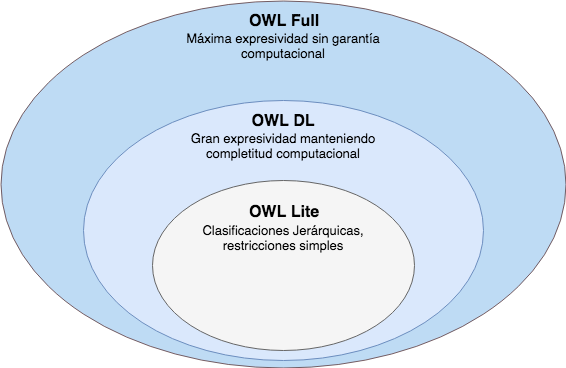
\includegraphics[width=150mm]{figuras/Diagramas-OwlSubClasses.png}
    \caption{Subclases OWL. \cite{owllevels}}
    \label{img:subclases owl}
    \end{figure}

OWL DL posee todas las características de OWL Lite más sus propias complejidades. OWL Full posee las mismas características de OWL DL agregando otras que resultan en mayor complejidad.

\section{Metodologías para el desarrollo de Ontologías}

En este apartado se dará un resumen de las metodologías más utilizadas para la creación de una ontología; Ontology Development 101, OntoKnowledge , Methontology, y NeOn. Luego se realizará un análisis y elección según los requerimientos de este trabajo.

\subsection{Ontology Development 101}

Esta metodología describe una serie de pasos y recomendaciones a la hora de crear una ontología. 

Se describen a continuación los pasos:
\begin{description}
\item[Paso 1:] Determinar el dominio y alcance de la ontología.
\item[Paso 2:] Considerar la reutilización de ontologías.
\item[Paso 3:] Enumerar términos importantes de la ontología.
\item[Paso 4:] Definir las clases y las jerarquías de las clases.
\item[Paso 5:] Definir las propiedades de las clases.
\item[Paso 6:] Definir las características de cada clase y propiedad.
\item[Paso 7:] Crear instancias.
\end{description}

Además la guía propone algunas buenas prácticas de desarrollo de ontologías relacionadas a la definición de clases como la correcta creación de jerarquías, herencias múltiples,  cuándo crear una clase o una propiedad, cuando es una instancia o una clase, etc. También algunos delineamientos sobre las propiedades como valores por defecto, cardinalidad, etc. Por último, una serie de convenciones de nombres dentro de la ontología. La metodología no tiene en cuenta el proceso de especificación ni el mantenimiento de la ontología.

\subsection{OntoKnowledge} 

Ontoknowledge propone crear ontologías teniendo en cuenta su uso posterior en sistemas de administración de conocimiento, por tanto las ontologías creadas son dependientes de la aplicación. La metodología incluye la identificación de metas a ser logradas a través de herramientas de control basadas en los escenarios de usos.

El proceso que propone la metodología se puede resumir en los siguientes pasos:

\textbf{Estudio de Factibilidad.} Esta debe ser aplicada a toda la aplicación y debe llevarse a cabo antes del desarrollo de la ontología. Aquí se identifica el problema y las áreas de oportunidades, se selecciona la mejor área de enfoque para la solución.

\textbf{Patada Inicial.} El resultado de este proceso es el Documento de Especificación de Requerimientos de la Ontología (ORSD). Se describen las metas y el dominio de la ontología, líneas de diseño (convenciones de nombres), lista de recursos disponibles (libros, revistas, documentación, etc), potenciales usuarios y casos de uso, así como las aplicaciones que utilizarán la ontología. Para esto se propone crear una lista de preguntas de competencia las cuales debe satisfacer la ontología creada. Los conceptos y relaciones más importantes son identificados en un nivel informal. También se debe de buscar ontologías para su potencial reuso, la metodología no provee un delineamiento para identificar dichas ontologías.

\textbf{Refinamiento.} Aquí se construye una ontología sólida orientada a la aplicación acorde al proceso de especificación. Este proceso se divide en dos actividades:

\begin{description}
\item[Actividad 1:] Extracción del conocimiento del los expertos del dominio. Los axiomas de la ontología son definidos y modelados por los expertos del dominio. La metodología propone el uso de una representación intermedia para modelar el conocimiento.
\item[Actividad 2:] Formalización de la ontología. La ontología es implementada en un lenguaje ontológico, el lenguaje es seleccionado según los requerimientos del uso de la ontología.
\end{description}

\textbf{Evaluación.} Este paso sirve para probar la usabilidad de la ontología desarrollada dentro del entorno para la cual fue desarrollada. En este proceso se verifica que se puedan responder las preguntas de competencia y que se satisfagan los requerimientos, además se prueba la ontología en el entorno de software para el cual se desarrolló.

\textbf{Mantenimiento.} En esta etapa es importante recalcar quién es el responsable de mantener la ontología y cómo se debe hacerlo.

La metodología propone un ciclo de vida incremental y cíclico como se muestra en la Figura \ref{img:ontoknowledge}.

\begin{figure}[h!]
    \centering
    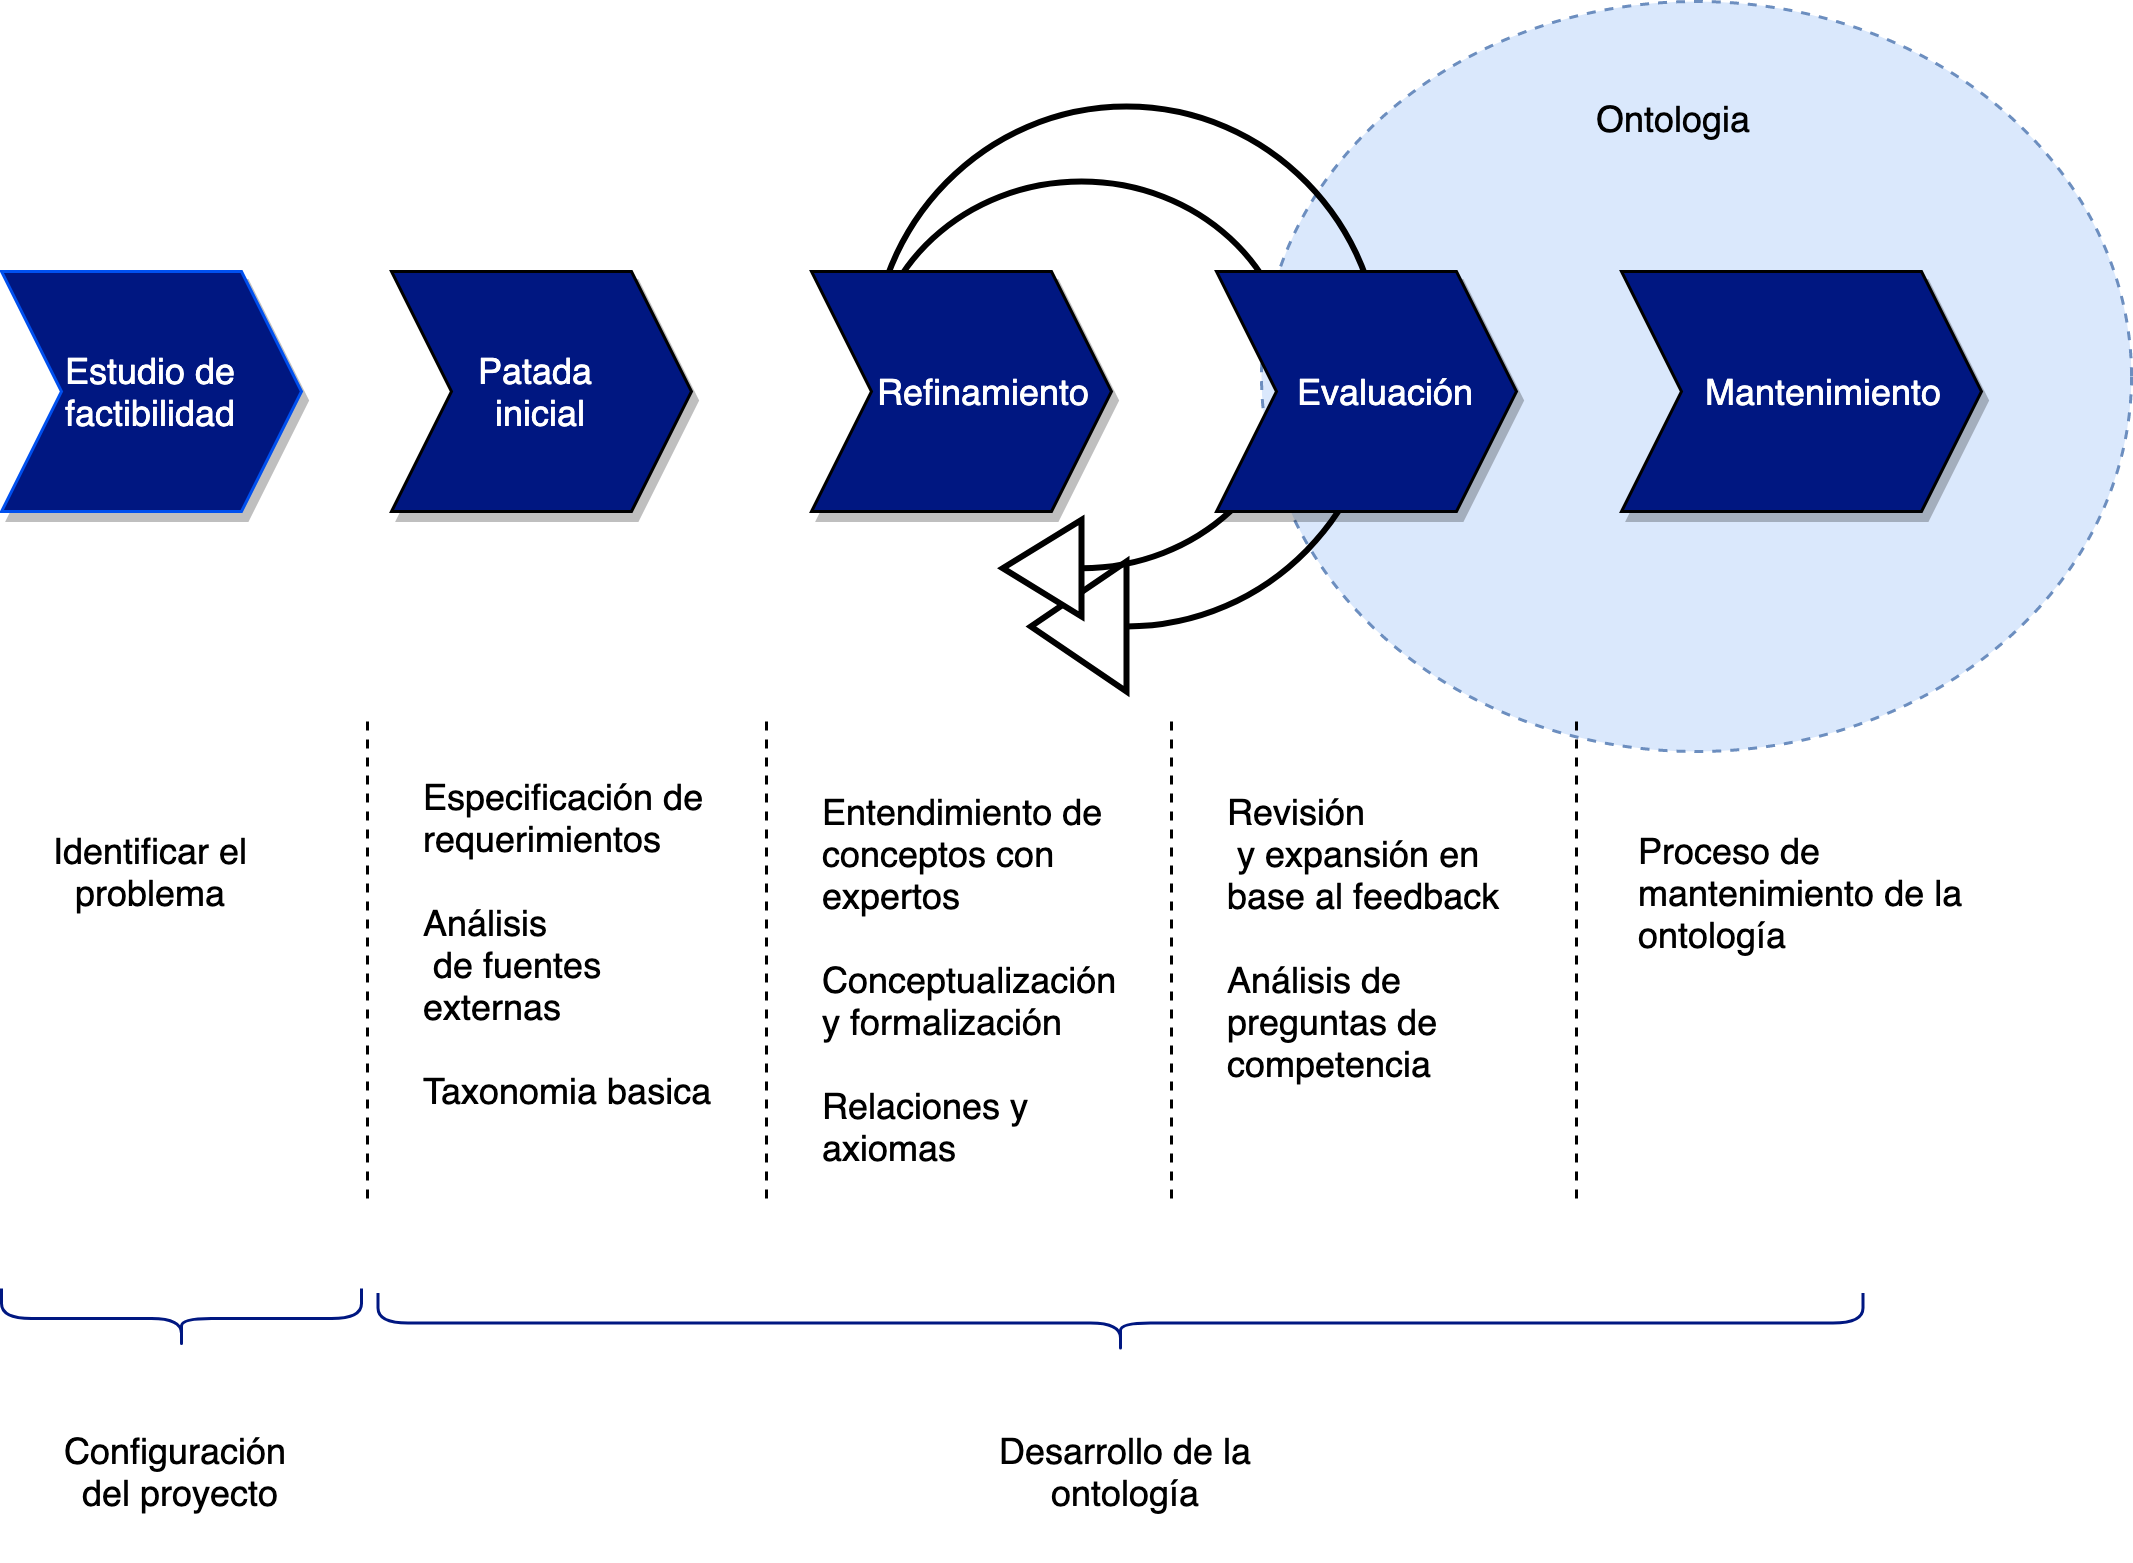
\includegraphics[width=150mm]{figuras/Diagramas-OntoKnowledgeProcess}
    \caption{Ciclo de vida de OntoKnowledge}
    \label{img:ontoknowledge}
    \end{figure}

\subsection{Methontology}

Esta metodología incluye la identificación del proceso del desarrollo de una ontología, que consiste en una serie de actividades, el ciclo de vida basado en el refinamiento de un prototipo y técnicas para llevar a cabo cada actividad durante el mantenimiento, el desarrollo y el soporte de las actividades. Todas las actividades están basadas en el proceso de desarrollo de software y las utilizadas en metodologías de ingeniería de conocimiento.

En la Figura \ref{img:methontology} se puede ver los estados de todo el ciclo de vida de la ontología.

\begin{figure}[h!]
    \centering
    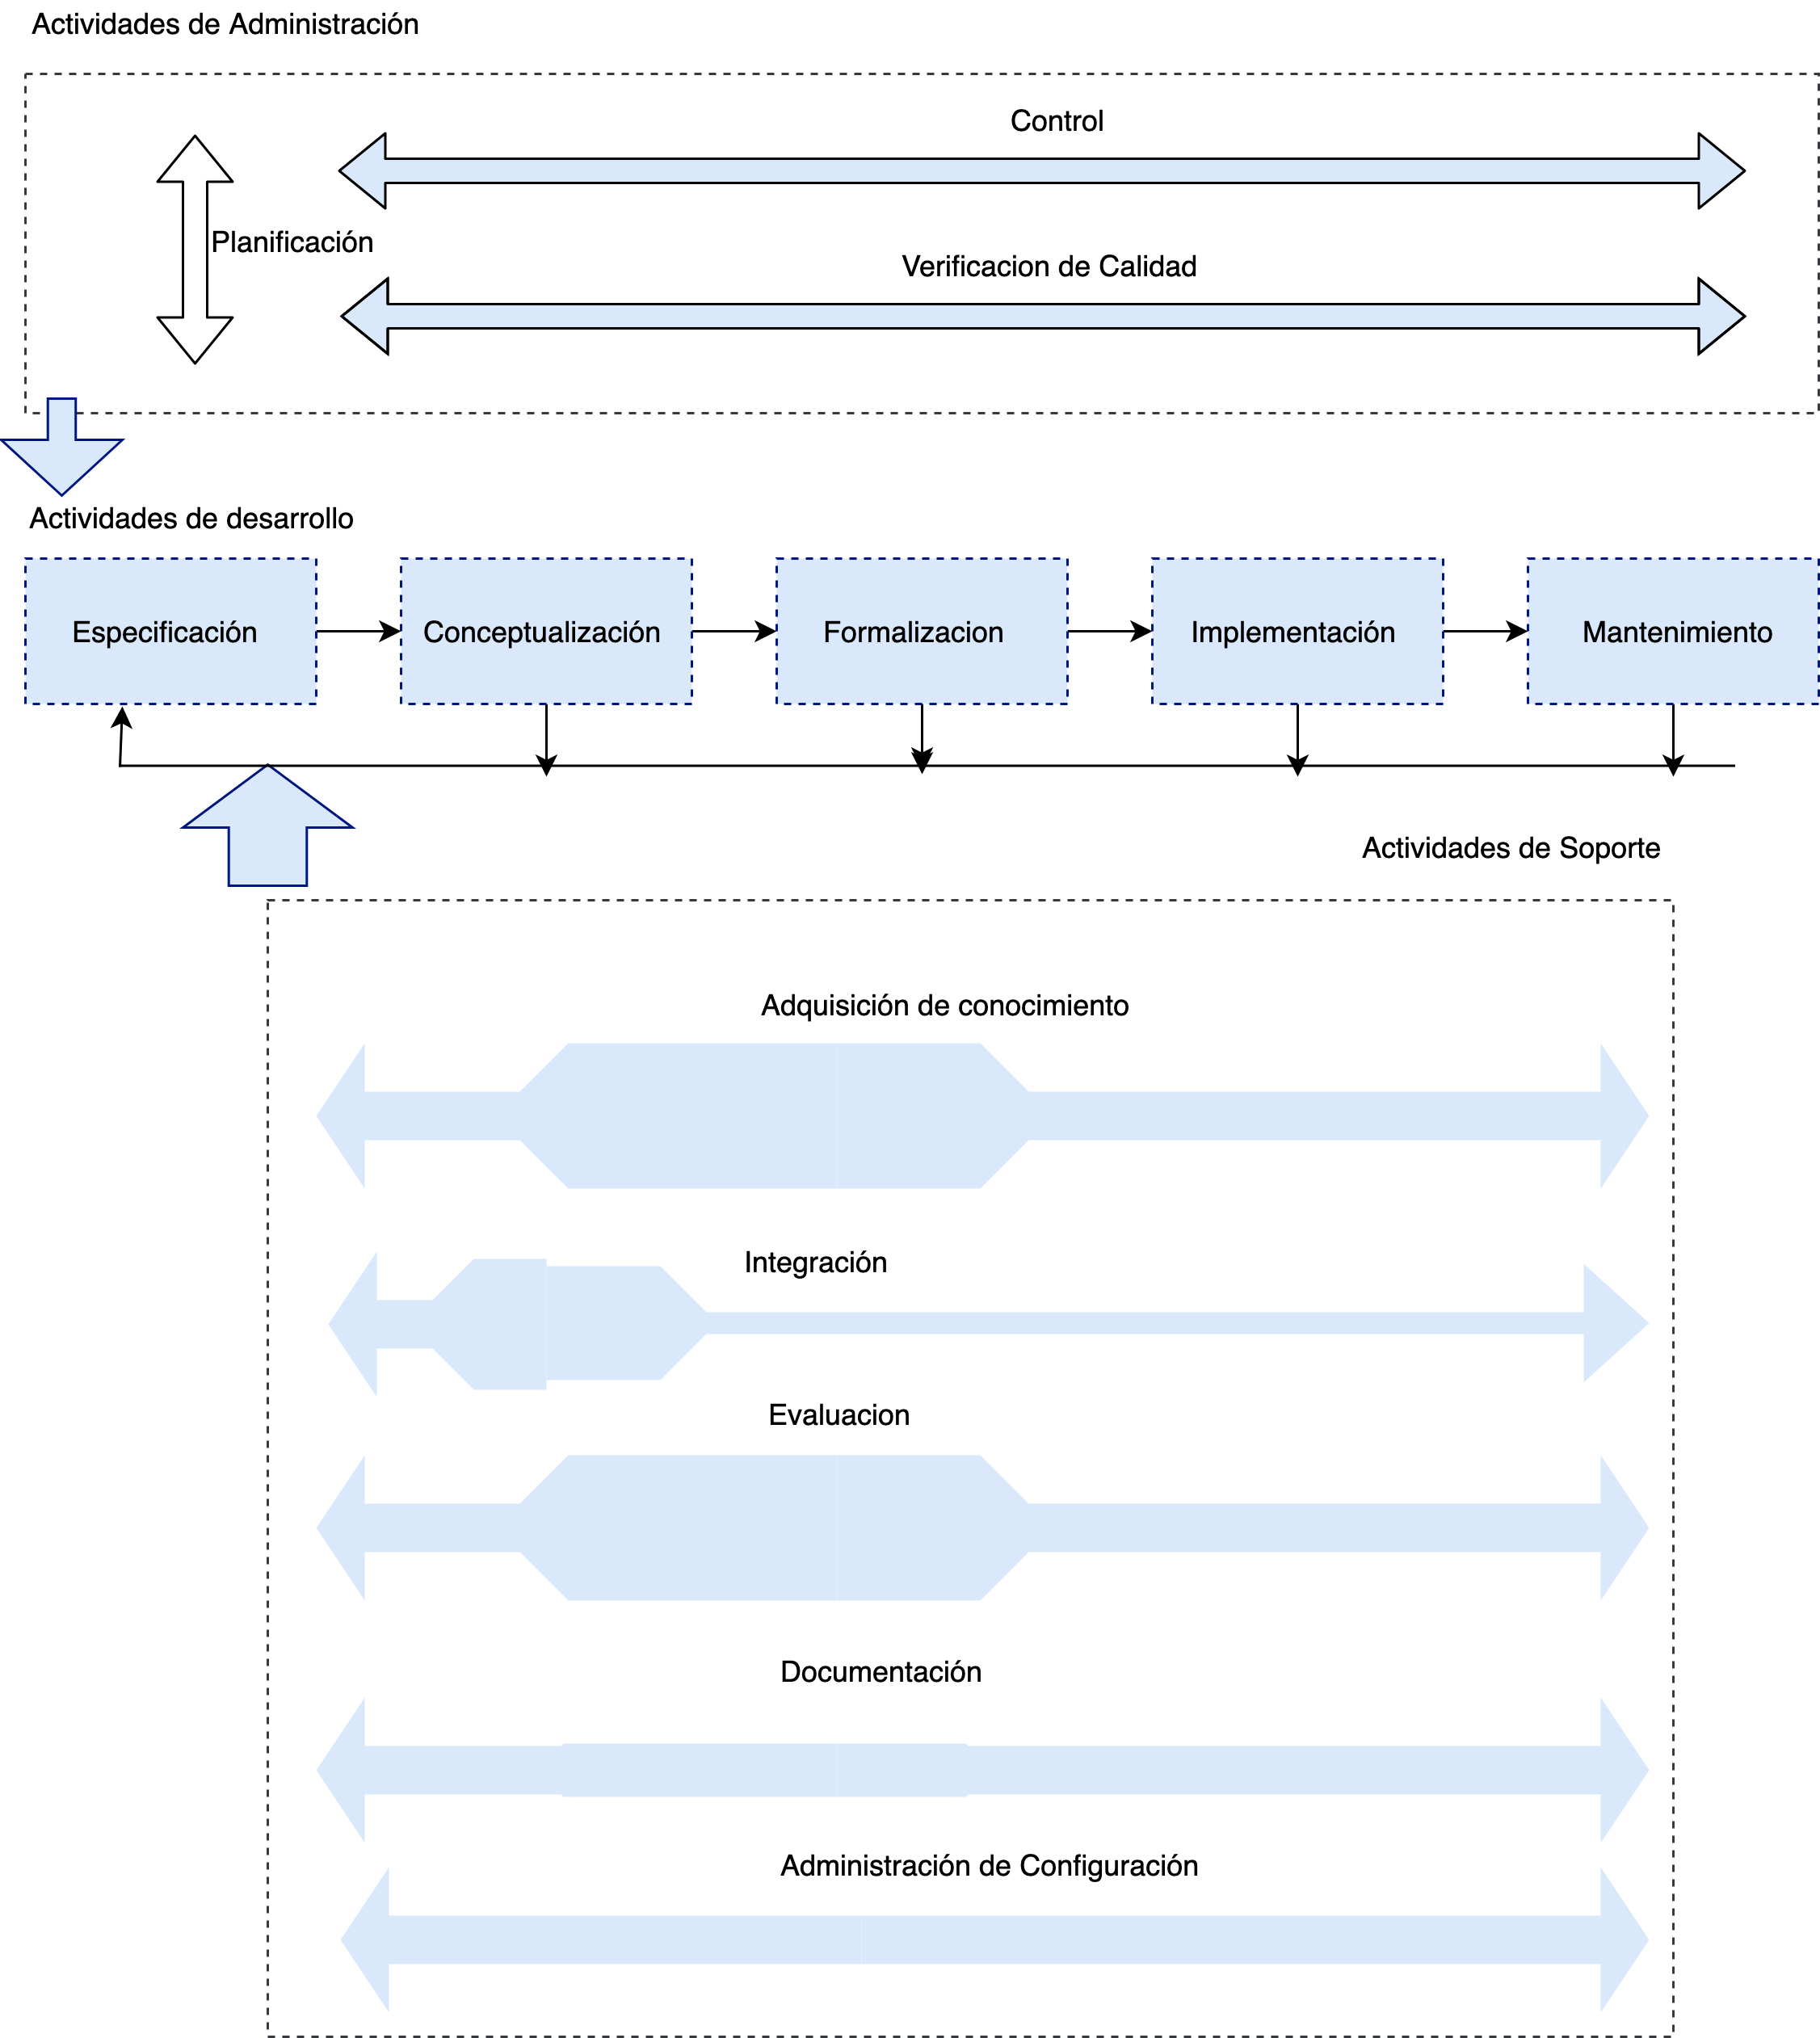
\includegraphics[width=150mm]{figuras/Diagramas-MethontologyProcess}
    \caption{Ciclo de vida de Methontology}
    \label{img:methontology}
    \end{figure}
    
    
La metodología propone un ciclo de vida basado en prototipos que permite agregar, cambiar y remover términos en cada prototipo. Para cada prototipo, se propone comenzar con la planificación para identificar las tareas, tiempos y recursos necesarios. Luego, comienza la actividad de especificación, con ella comienzan las actividades de gestión (Control y Calidad) y procesos de soporte (Adquisición de conocimiento, integración, evaluación, documentación y gestión de la configuración), todo esto ejecutado en forma paralela a las actividades de desarrollo (especificación, conceptualización, implementación y mantenimiento) durante todo el ciclo de vida de la tecnología \cite{fernandez1997methontology}.
 
A continuación se describen algunas de las principales actividades:

\begin{enumerate}
\item \textbf{Especificación:} Especificar el propósito de la ontologías, esto incluye usuarios, contexto, nivel de formalidad esperado y granularidad. El resultado de esta fase es un documento de especificación de la ontología en lenguaje natural.
\item \textbf{Adquisición} de conocimiento: Esto ocurre en paralelo a las demás fases, pero específicamente en la parte de especificación. Se consultan libros, manuales, tablas, otras ontologías y expertos para adquirir conocimientos sobre el área a modelar.
\item \textbf{Conceptualización:} Se identifican los términos según sean conceptos, instancias, relaciones o propiedades para crear un modelo conceptual del dominio.
\item \textbf{Integración:} En esta fase se considera el reuso de términos de otras ontologías para no volver a definir y ahorrar trabajo.
\item \textbf{Implementación:} La ontología es representada formalmente en un lenguaje tipo OWL o RDFS.
\item \textbf{Evaluación:} Significa hacer un juzgamiento técnico de la ontología creada, el entorno de desarrollo y la documentación de la misma. La evaluación está compuesta por la verificación y la validación.
\item \textbf{Documentación:} El cual consiste en todos los documentos producidos durante el desarrollo de la ontología que va desde el mismo código de la ontología hasta artículos científicos de la misma.
\end{enumerate}


\subsection{NeOn}
Esta metodología incluye métodos, técnicas y herramientas para llevar a cabo actividades para el proceso de desarrollo de una red ontológica. Está enfocada en la especificación de los requerimientos, la planificación y el reuso de recursos ontológicos y no-ontológicos \cite{suarez2010neon}.

La metodología presenta los siguientes componentes:
\begin{itemize}
    \item Un glosario: Identifica y define los procesos y actividades que pueden estar dentro de el desarrollo de una ontología. En la Figura \ref{img:neon actividades} se muestra la lista de procesos y actividades divididas según la fase de desarrollo.
    \item Nueve escenarios para el desarrollo de ontologías. Se identificaron nueve escenarios flexibles para el desarrollo de ontologías, donde cada escenario está compuesto de diferentes procesos y actividades. En la Figura \ref{img:neon ciclo de vida} se distinguen las relaciones entre las actividades y los escenarios donde las fechas dirigidas con círculos numerados asociados representan los diferentes escenarios. 
    \item Una serie de guías metodológicas para procesos y actividades como el reuso de recursos ontológicos y no-ontológicos, la especificación de los requerimientos, la planificación, etc. Los procesos y actividades están representados en la Figura \ref{img:neon ciclo de vida} con cajas y círculos de color.
\end{itemize}

A continuación se presenta el glosario de términos:
\begin{figure}[h!]
    \centering
    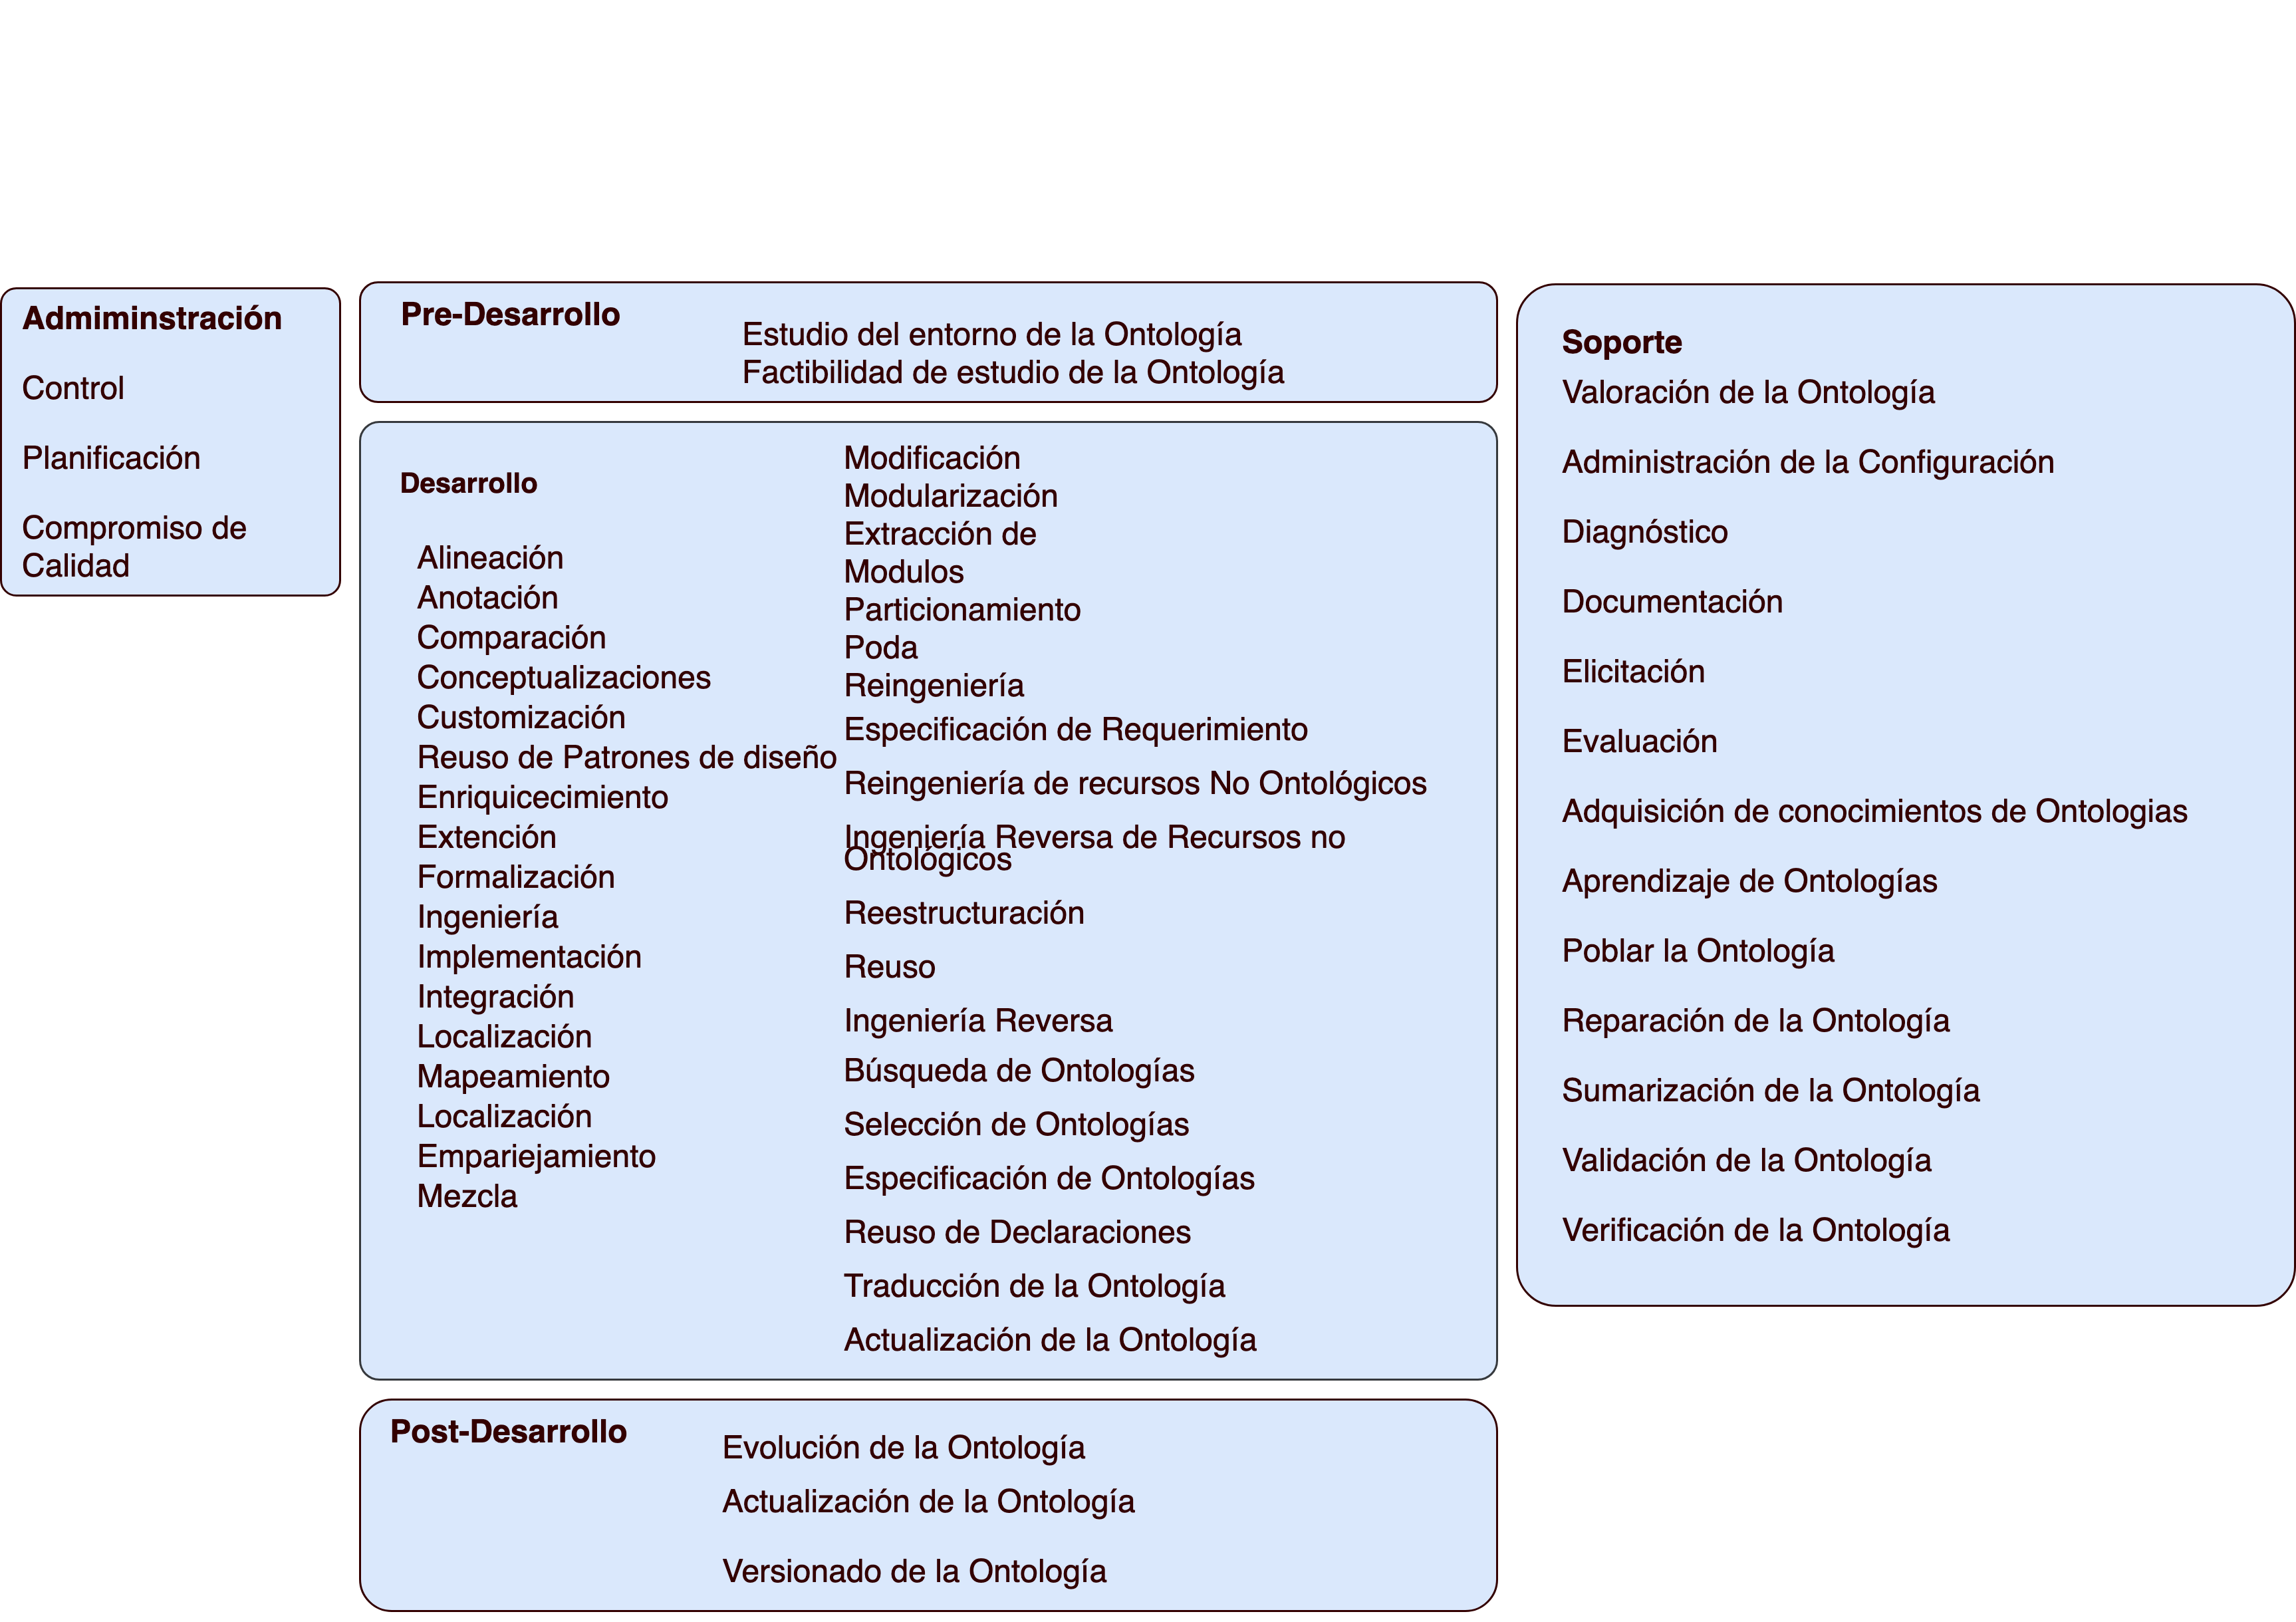
\includegraphics[width=150mm]{figuras/Diagramas-NeonActivities}
    \caption{Actividades de NeOn}
    \label{img:neon actividades}
    \end{figure}


A continuación se presentan los nueve escenarios que propone NeOn.

\begin{description}
    \item[Escenario 1] El escenario va desde la especificación hasta la implementación. La ontología es desarrollada desde el principio, esto significa sin utilizar ninguna base de conocimiento ya construida.
    \item[Escenario 2] Reuso y Reingeniería de recursos no-ontológicos. Este escenario cubre el caso donde los desarrolladores analizan recursos no-ontológicos, y deciden según los requerimientos, qué recurso no-ontológico se puede reutilizar para construir esta ontología. Este escenario también realiza una reingeniería del recurso seleccionado.
    \item[Escenario 3] Reuso de recursos ontológicos. En este escenario los desarrolladores reusan recursos ontológicos, esto se puede hacer de tres maneras: reuso total, reuso de módulos y/o reuso de sentencias.
    \item[Escenario 4] Reuso y reingeniería de recursos ontológicos.Aquí, los desarrolladores hacen tanto un reuso como una reingeniería de los recursos ontológicos.
    \item[Escenario 5] Reuso y unión de recursos ontológicos. Este escenario es propicio cuando se eligen muchas ontologías del mismo dominio de conocimiento para reutilizar y se quiere crear una nueva ontología a partir de ellas.
    \item[Escenario 6] Reuso, unión y reingeniería de recursos ontológicos. Similar al escenario 5, aquí los desarrolladores realizan un proceso de reingeniería antes de unir los recursos reutilizados.
    \item[Escenario 7] Reusos de patrones de diseño de ontologías (ODP). En este escenario se utilizan repositorios de ODP para reutilizarlos.
    \item[Escenario 8] Reestructuración de recursos ontológicos. Se reestructuran recursos ontológicos, esto significa modularizar, recortar, extender y/o especializar el recurso ontológico para integrarla a la ontología construida.
    \item[Escenario 9] Localización de un recurso ontológico. En este escenario se adapta una ontología a otros lenguajes u otras culturas o comunidades, produciendo así una ontología multilenguaje.
\end{description}

\begin{figure}[h!]
    \centering
    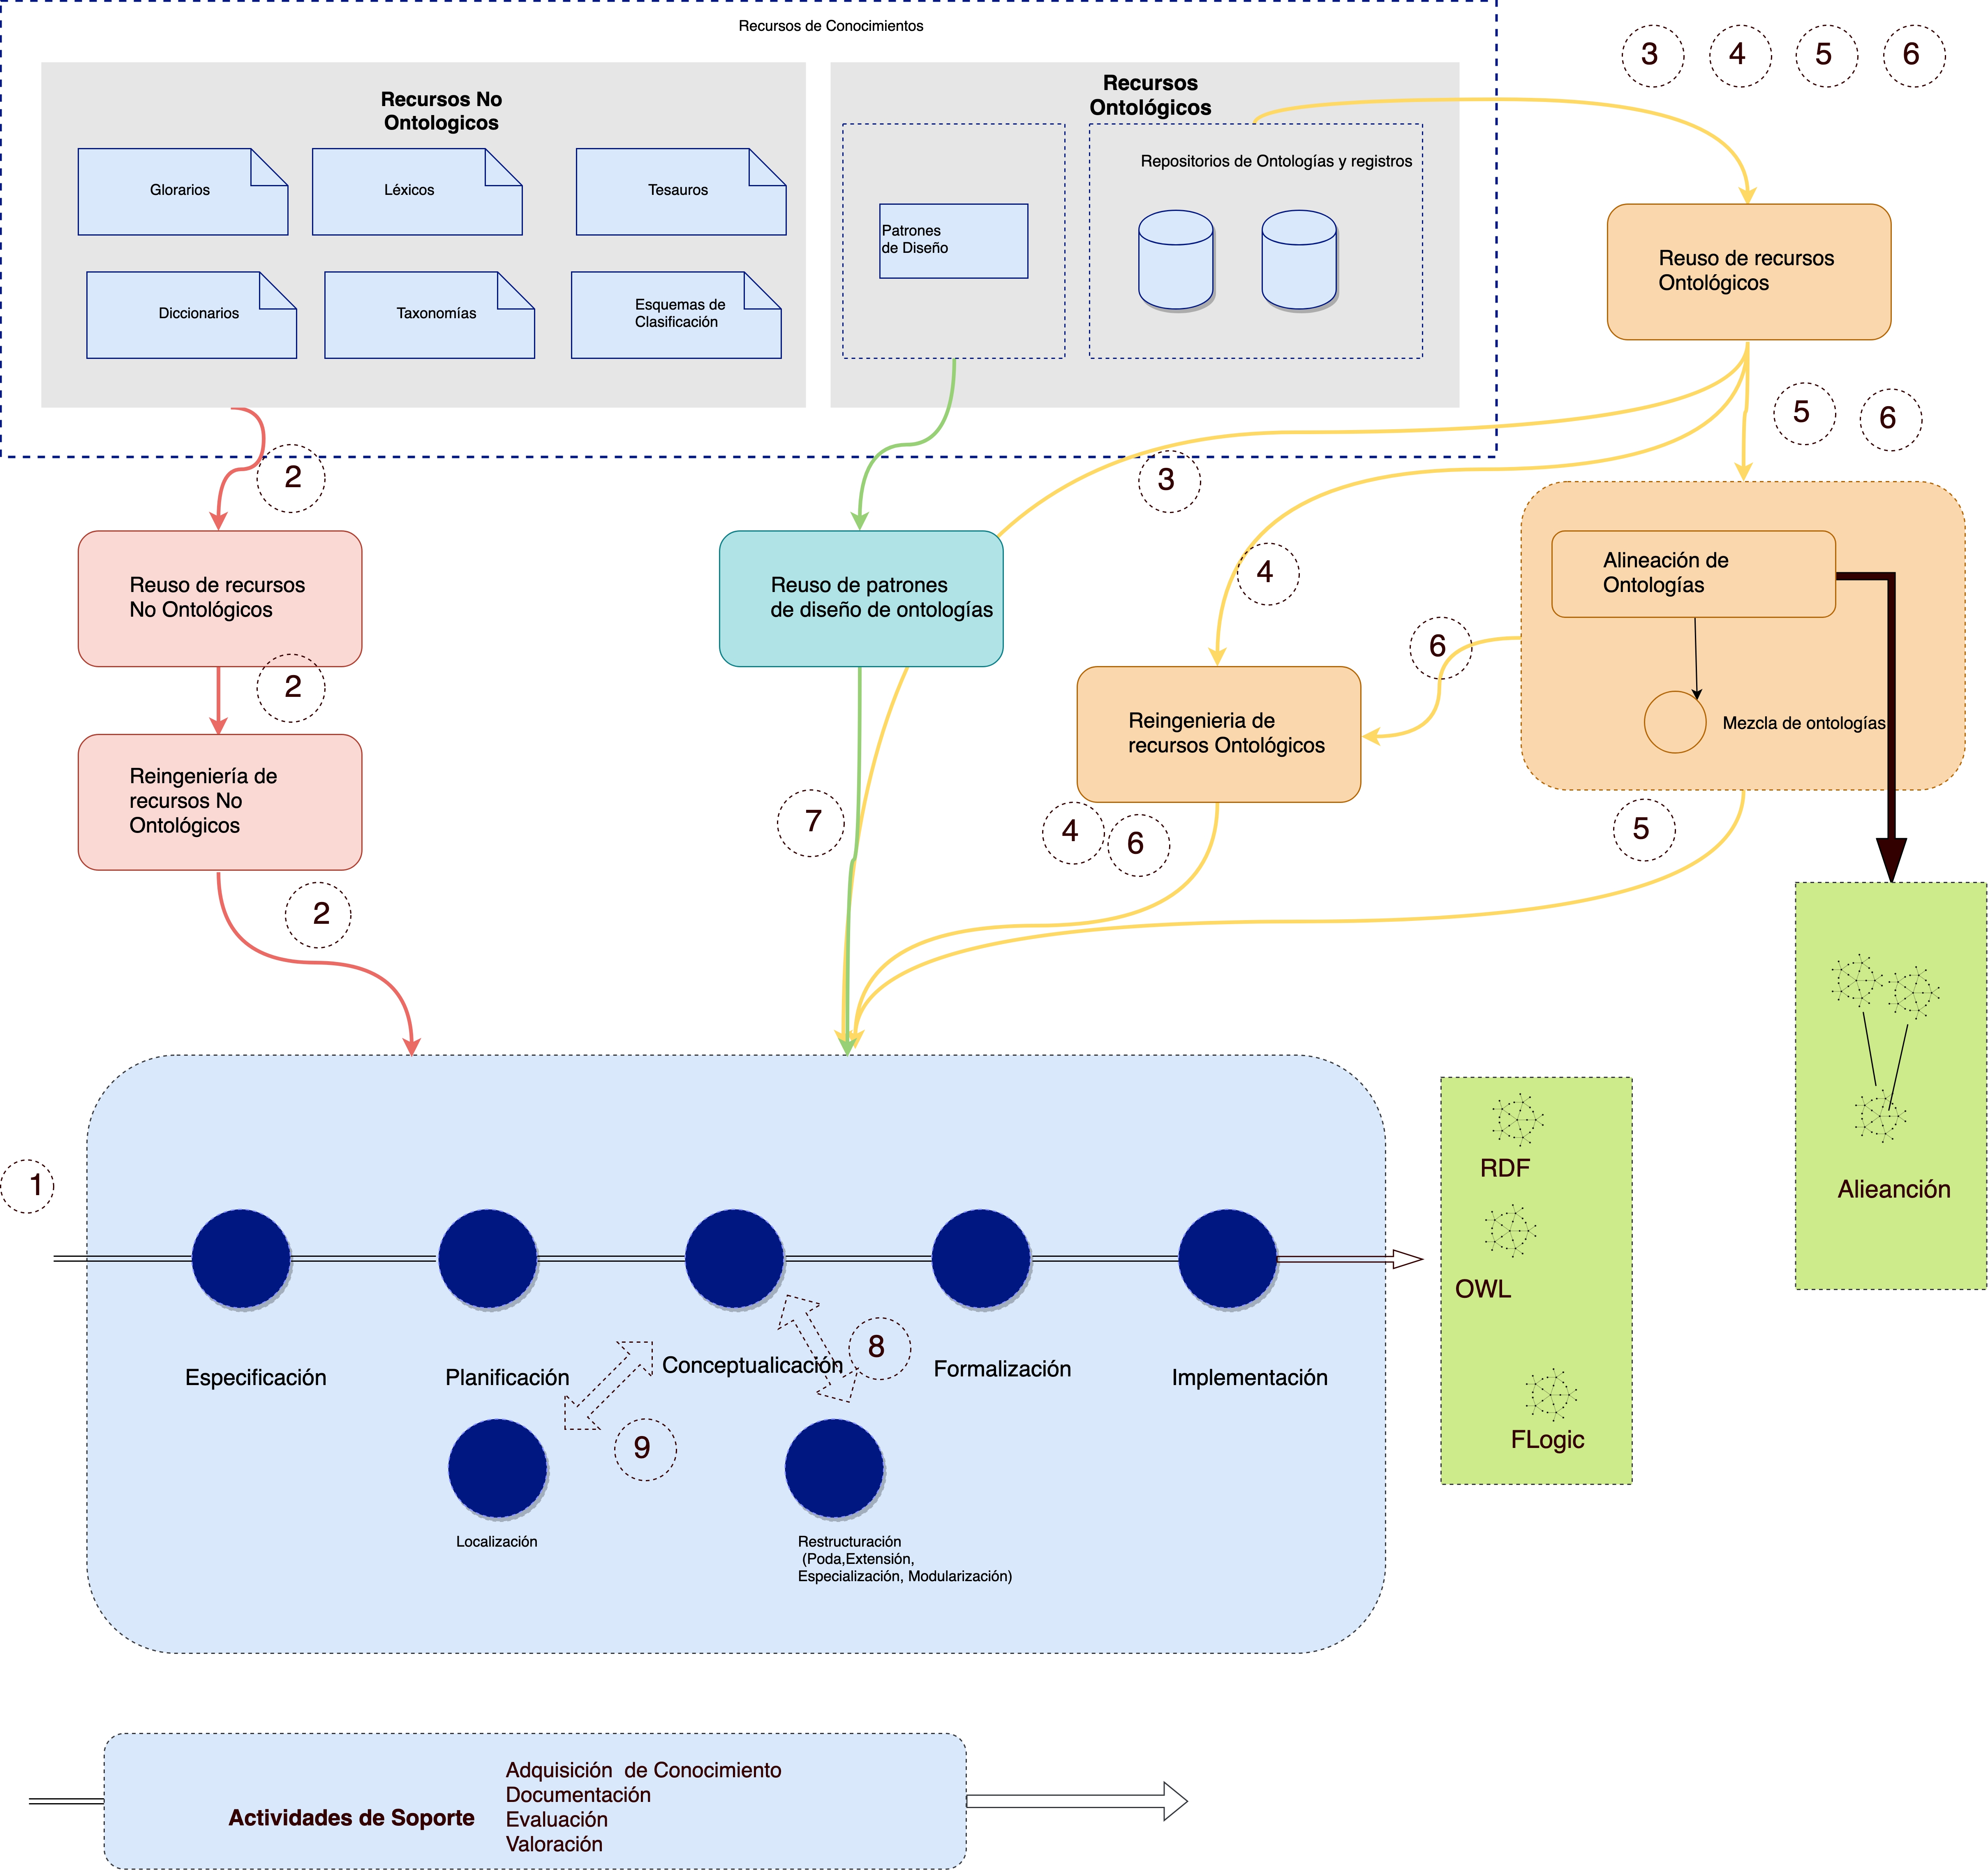
\includegraphics[width=150mm]{figuras/Diagramas-NeonProcess}
    \caption{Ciclo de vida de NeOn}
    \label{img:neon ciclo de vida}
    \end{figure}

El proceso de desarrollo de una ontología es definido como un proceso en el cual las necesidades de un usuario son convertidas a una ontología. Esto significa que el proceso se puede ver como un caso específico del proceso de desarrollo de software.	
El ciclo de vida es un modelo que describe cómo construir y mantener un proyecto ontológico, osea cómo ordenar los procesos y actividades en fases. Se pueden tener dos tipos de ciclo de vida que son:

\begin{itemize}
    \item Modelo de ciclo de vida de tipo cascada: En este modelo cada fase debe ser culminada antes de avanzar a la siguiente, no se permite retroceso excepto en el caso de la fase de mantenimiento. Este modelo es ideal cuando el tiempo de desarrollo es acotado y el dominio de conocimiento a modelar es bien conocido.
    \item Modelo de ciclo de vida de tipo iterativo-incremental: cada iteración es similar al modelo de cascada. Es ideal cual existe mucha incertidumbre acerca del alcance de la ontología a modelar.
\end{itemize}

A continuación exponemos los 5 modelos de ciclo de vida:	

\begin{description}
    \item[Modelo cascada de 4 fases.] Representa las etapas de una red de ontologías, comenzando con la Fase de Iniciación y yendo a través de la Fase de Diseño y Fase de Implementación hasta la Fase de Mantenimiento.
    \item[Modelo cascada de 5 fases.] Extiende el modelo de 4 fases con el reuso de recursos  ontológicos tales como son.
    \item[Modelo cascada de 5 fases + mezcla.] Es un caso especial del modelo de 5 fases. Incluye la Fase de Mezcla para obtener un nuevo recurso ontológico a partir de dos o más recursos ontológicos previamente seleccionados en la Fase de Reuso.
    \item[Modelo cascada de 6 fases.] Extiende el modelo de 5 fases con la Fase de Reingeniería. Permite la reingeniería de recursos de conocimiento (ontológicos y no-ontológicos). Puede ocurrir que algunos recursos de conocimiento son transformados en ontologías en la Fase de Reingeniería.
    \item[Modelo cascada de 6 fases + Mezcla.] Extiende el modelo de 6 fases incluyendo la Fase de Mezcla luego de la Fase de Reuso.
\end{description}

Los escenarios están ligados a un modelo dentro del ciclo de vida, como se muestra en la Tabla \ref{escenarios vs modelo}.

\begin{table}[tbp]
\centering
\caption{Escenarios vs Modelo}
\label{escenarios vs modelo}
\resizebox{15cm}{!} {
\begin{tabular}{|l|C|c|c|c|c|}
\hline
 & \multicolumn{1}{|m{2cm}|}{Modelo de 4-fases} & \multicolumn{1}{|m{2cm}|}{Modelo de 5-fases} & \multicolumn{1}{|m{2cm}|}{Modelo de 5-fases + mezcla} & \multicolumn{1}{|m{2cm}|}{Modelo de 6-fases} & \multicolumn{1}{|m{2cm}|}{Modelo de 6-fases + mezcla} \\ \hline
 Escenario 1 & x & & & & \\ \hline
 Escenario 2 & \multicolumn{1}{|m{2cm}|}{} & \multicolumn{1}{|m{2cm}|}{} & \multicolumn{1}{|m{2cm}|}{} & \multicolumn{1}{|m{2cm}|}{x} & \multicolumn{1}{|m{2cm}|}{} \\ \hline
 Escenario 3 & \multicolumn{1}{|m{2cm}|}{} & \multicolumn{1}{|m{2cm}|}{x} & \multicolumn{1}{|m{2cm}|}{} & \multicolumn{1}{|m{2cm}|}{} & \multicolumn{1}{|m{2cm}|}{} \\ \hline
 Escenario 4 & \multicolumn{1}{|m{2cm}|}{} & \multicolumn{1}{|m{2cm}|}{} & \multicolumn{1}{|m{2cm}|}{} & \multicolumn{1}{|m{2cm}|}{x} & \multicolumn{1}{|m{2cm}|}{} \\ \hline
 Escenario 5 & \multicolumn{1}{|m{2cm}|}{} & \multicolumn{1}{|m{2cm}|}{} & \multicolumn{1}{|m{2cm}|}{x} & \multicolumn{1}{|m{2cm}|}{} & \multicolumn{1}{|m{2cm}|}{} \\ \hline
 Escenario 6 & \multicolumn{1}{|m{2cm}|}{} & \multicolumn{1}{|m{2cm}|}{} & \multicolumn{1}{|m{2cm}|}{} & \multicolumn{1}{|m{2cm}|}{} & \multicolumn{1}{|m{2cm}|}{x} \\ \hline
 Escenario 7 & \multicolumn{1}{|m{2cm}|}{} & \multicolumn{1}{|m{2cm}|}{} & \multicolumn{1}{|m{2cm}|}{} & \multicolumn{1}{|m{2cm}|}{x} & \multicolumn{1}{|m{2cm}|}{} \\ \hline
 Escenario 8 & \multicolumn{1}{|m{2cm}|}{} & \multicolumn{1}{|m{2cm}|}{} & \multicolumn{1}{|m{2cm}|}{x} & \multicolumn{1}{|m{2cm}|}{} & \multicolumn{1}{|m{2cm}|}{} \\ \hline
 Escenario 9 & \multicolumn{1}{|m{2cm}|}{} & \multicolumn{1}{|m{2cm}|}{} & \multicolumn{1}{|m{2cm}|}{x} & \multicolumn{1}{|m{2cm}|}{} & \multicolumn{1}{|m{2cm}|}{} \\ \hline
\end{tabular}
}
\end{table}



\section{Herramientas tecnológicas}
En esta sección presentaremos las herramientas tecnológicas estudiadas para el desarrollo de este trabajo. Se presenta un editor de ontologías llamado Protégé (ver \ref{subsection:protege}), un visualizador de ontologías en formato de grafo llamado VOWL (ver \ref{subsection:vowl}), un framework para la manipulación de datos en RDF, RDFS y OWL llamado Apache Jena (ver \ref{subsection:jena}) y una herramienta para realizar consultas SPARQL llamado Apache Jena Fuseki (ver \ref{subsection:fuseki}) .
\subsection{Protégé}
\label{subsection:protege}
Protégé es una herramienta de código libre para desarrolladores de ontologías y permite crear sistemas de base de conocimientos. El editor consiste en una interfaz gráfica de usuario donde podemos crear y editar clases, instancias, propiedades y restricciones. Nos permite guardar la ontología en varios formatos como XML, RDF, TTL y OWL. En la Figura \ref{img:protege} se muestra una captura de pantalla de la herramienta.

\begin{figure}[h!]
    \centering
    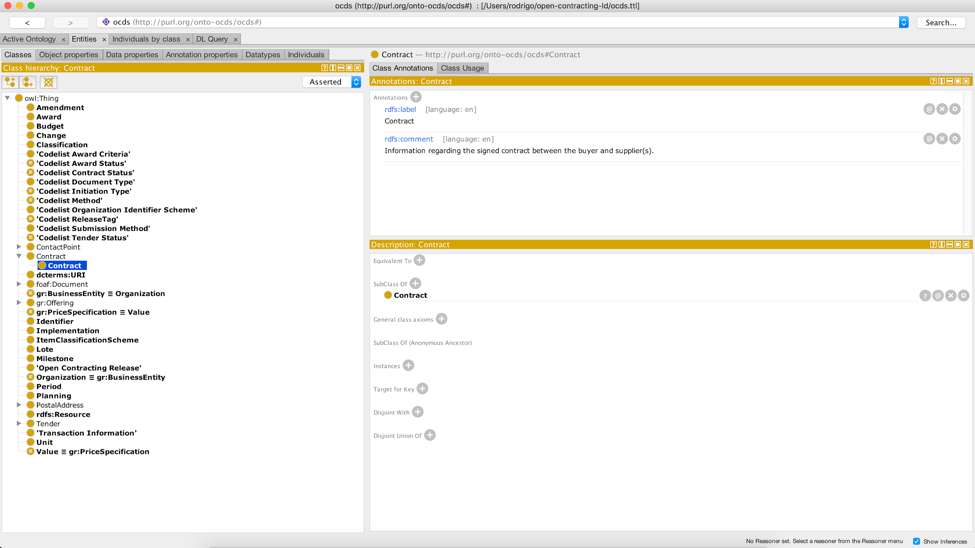
\includegraphics[width=150mm]{figuras/protege}
    \caption{Herramienta de Desarrollo de Ontologías: Protégé}
    \label{img:protege}
    \end{figure}

\subsection{Visual Notation for OWL}
\label{subsection:vowl}
Además se utilizó una herramienta de visualización gráfica de ontologías llamada \textit{Visual Notation for OWL} (VOWL) en su versión Web para visualizar de forma gráfica las ontologías estudiadas, en la Figura \ref{img:webvowl} se presenta una captura de pantalla de la herramienta utilizando como ejemplo una ontología llamada FOAF.

\begin{figure}[h!]
    \centering
    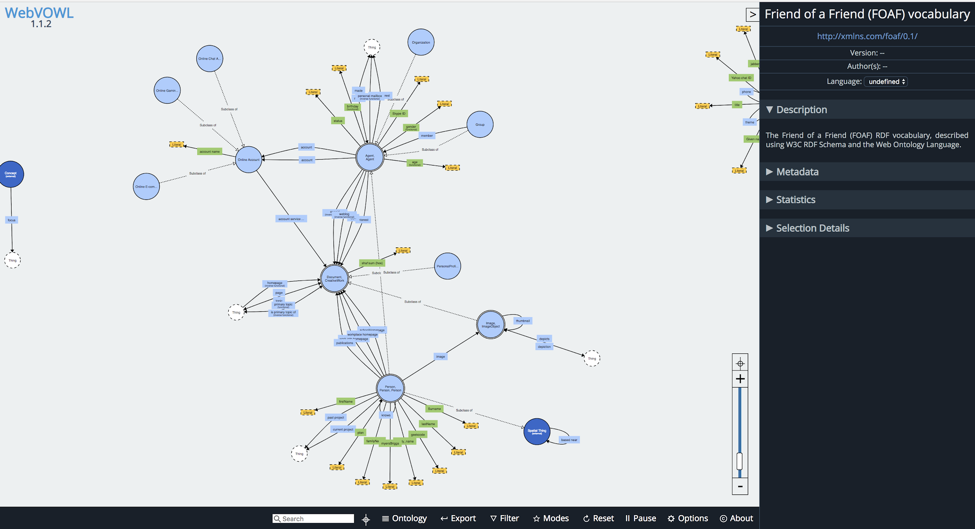
\includegraphics[width=150mm]{figuras/webvowl}
    \caption{Herramienta de Visualización de Ontologías: WebVOWL}
    \label{img:webvowl}
    \end{figure}
    

\subsection{Apache Jena}
\label{subsection:jena}
Jena es un \textit{Framework} implementado en JAVA para construir aplicaciones de la Web Semántica. Provee una librería para la manipulación de datos en RDF, RDFS, RDFa, OWL y SPARQL, y está alineada con las recomendaciones de la W3C. Jena incluye un motor de inferencias basado en reglas para realizar los razonamientos basados en OWL y RDFS, además de una variedad de estrategias para el almacenamiento de triplas RDF en memoria y en disco.

\subsection{Consulta de datos con SPARQL}
\label{subsection:fuseki}
Para consultar triplas basadas en RDF han surgido varios lenguajes de consulta, pero SPARQL es el más ampliamente utilizado y fue estandarizado por la W3C \cite{SPARQLDpoc:online}. Una consulta SPARQL es formulada usando patrones de grafos que pueden ser combinados con operaciones algebraicas como unión, opcional, filtro, etc. El resultado de la consulta es una lista de relaciones que pueden estar expresadas en tablas o en RDF.

A forma de explicar la semántica y sintaxis completa de este lenguaje, en el Cuadro \ref{lst:consulta-sparql} se muestra en un ejemplo la utilización del lenguaje realizando una consulta básica a la base de datos de DBPEDIA \cite{DBpedia:online} donde se listaron los nombres, fechas de nacimiento, fallecimiento y las URIs de personas nacidas en Paraguay antes de 1900, ordenadas por nombre.\hfill \break

\lstset{
    language=SPARQL
}
\noindent\begin{minipage}{\textwidth}
\begin{lstlisting}[captionpos=b, caption=Ejemplo de consulta SPARQL, label=lst:consulta-sparql,  numbers=left,  numberstyle=\tiny\color{mygray},
    basicstyle=\footnotesize\ttfamily,frame=single]
PREFIX dbo: <http://dbpedia.org/ontology/>
PREFIX xsd: <http://www.w3.org/2001/XMLSchema#>
PREFIX foaf: <http://xmlns.com/foaf/0.1/>
PREFIX : <http://dbpedia.org/resource/>

SELECT ?name ?birth ?death ?person WHERE { 

?person dbo:birthPlace :Paraguay . 
?person dbo:birthDate ?birth . 
?person foaf:name ?name . 
?person dbo:deathDate ?death . 
FILTER (?birth < "1900-01-01"^^xsd:date) . 

}
ORDER BY ?name
 
\end{lstlisting}
\end{minipage}

En las líneas 1 al 4 se pueden ver los prefijos de las ontologías utilizadas en la consulta, luego se presentan las triplas que componen las restricciones de la consulta. Está fuera del alcance de este documento la explicación detallada de la sintaxis de SPARQL.

Apache Jena Fuseki es un Servidor o Punto SPARQL que además provee un motor de inferencias. Se ejecuta como una aplicación web Java (archivo WAR). Provee el protocolo de consulta y actualización SPARQL 1.1 así como también el protocolo de \textit{SPARQL Graph Store}.

\section{Discusión del Capítulo}
En este capítulo se vieron los conceptos sobre Linked Open Data, Web Semántica y el rol de las ontologías en la misma. Además se dio una introducción a RDF, RDFS y OWL que son formas de representación de ontologías y datos en la Web Semántica. Para poder realizar consultas a las base de datos en RDF se dió una breve introducción del lenguaje SPARQL.

Se revisaron las metodologías más utilizadas para el desarrollo de una ontología para luego hacer una comparación de cada una de ellas presentadas en la Tabla \ref{tab:comparacion}. En cuanto a la madurez y completitud de cada una podemos decir que la metodología NeOn es la que mejor se posiciona, ya que la misma está basada en metodologías de desarrollo de software y metodologías de ingeniería de conocimiento. Además contempla escenarios de reuso de recursos ontológicos y no-ontológicos, los cuales serán necesarios para el desarrollo de este trabajo. Por este motivo se eligió NeOn como metodología base para el desarrollo de la ontología.

Además presentamos las herramientas tecnológicas utilizadas para el desarrollo de ontologías y posterior consulta a través de un servidor de consultas llamado Punto SPARQL.

En el siguiente capítulo comenzaremos con el desarrollo de la ontología utilizando la metodología NeOn.


%!TEX root = ../main.tex
\chapter{Desarrollo de la Ontología}
\label{chap:Desarrollo de la Ontologia}

Luego de haber estudiado las distintas metodologías para el desarrollo de ontologías, se decidió utilizar la metodología NeOn, ya que la misma según la tabla  xx posee mayor especificación en las actividades a desarrollar  y contempla los caso de reuso de recursos ontológicos y no-ontológicos. 

Siguiendo la metodología NeOn se identifica que la ontología a desarrollar sigue las actividades compuestas principalmente por los escenarios 1, 2 y 3 que se exponen en la metodología. El escenario 1, puesto que se quiere modelar una ontología desde el principio y es la base de los demás escenarios, el escenario 2 y 3 ya que se pretende reusar recursos ontológicos y no-ontológicos respectivamente. A continuación se detalla la primera actividad de la metadología, que consiste en la especificación de los requerimiento de la ontología.


\section{Especificación de requerimientos de la ontología}

En esta actividad se define el alcance y los requerimientos de la ontología a desarrollar. Como resultado de esta actividad se obtiene el Documento de Especificación de Requerimientos de la Ontología (ORSD). A continuación se detalla el resultado de dicho proceso.
\begin{enumerate}

    \begin{figure}[h!]
        \centering
        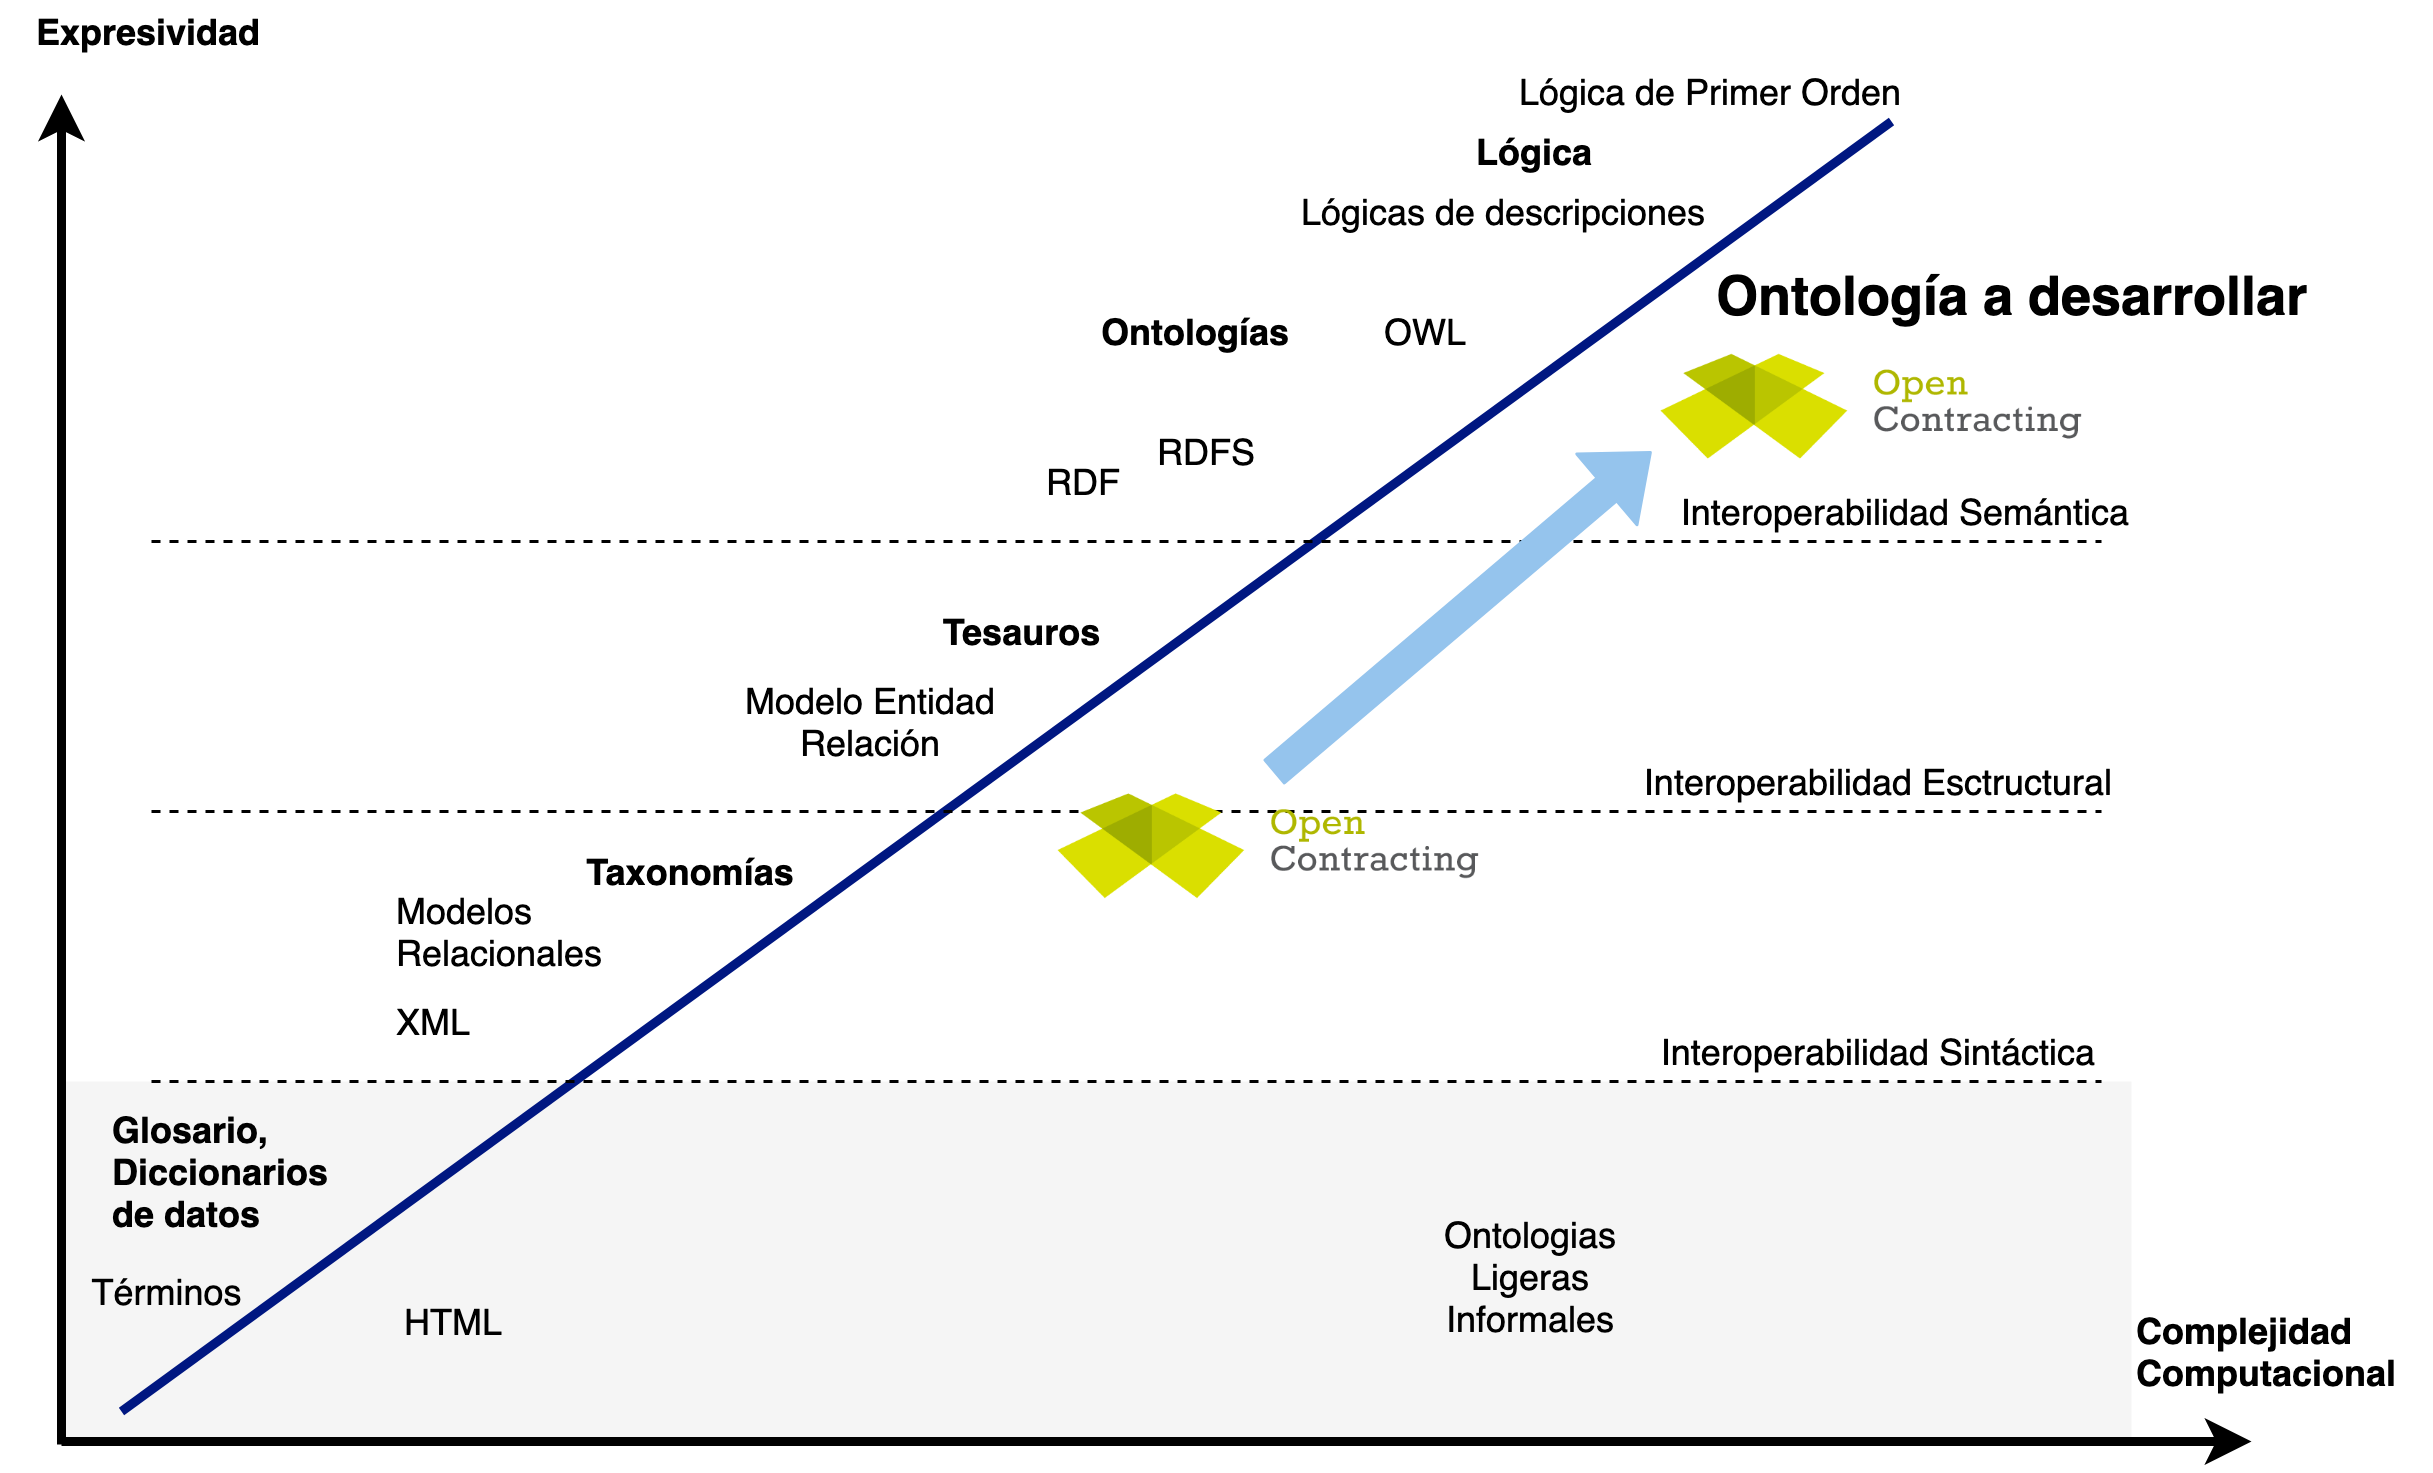
\includegraphics[width=150mm]{figuras/Diagramas-OenContracting.png}
        \caption{Nivel de complejidad semantica de la ontologia a desarrollar}
        \label{img:ocds-ocntology-complejidad}
        \end{figure}
        
\item \textbf{Propósito:} Crear una ontología para el dominio de Contrataciones Públicas para lograr la interoperabilidad semántica con otras fuentes de datos externas utilizando el OCDS como base de conocimiento principal aumentando la formalidad semántica como se muestra en la figura \ref{img:ocds-ocntology-complejidad}


\item \textbf{Alcance:} El alcance de la ontología está delimitada por el vocabulario detallado en la versión 1 del OCDS. Se eligió dicha versión ya en el momento del inicio de esta investigación era la última versión estable del estándar.
\item \textbf{Lenguaje de Implementación.} Se utilizará el lenguaje OWL debido a que es el lenguaje preferido para ontologías en la web semántica recomendado por la W3C \cite{OWLSeman72:online}, y se requiere de una ontología lo suficientemente ligera y explícita que se pueda manejar en la web semántica.
\item \textbf{Grupo Objetivo.}La ontología está orientada a:
\begin{enumerate}
    \item Expertos del dominio de Contrataciones Públicas que quieran realizar consultas ad-hoc sobre datos.
    \item Desarrolladores de software que deseen implementar el OCDS.
    \item Desarrolladores de software que necesiten integrar datos de contrataciones públicas con otras fuentes externas. \end{enumerate}
\item \textbf{Usos de la Ontología. }La ontología se utilizará para crear un esquema de publicación en JSON-LD, esto es debido a que la sintaxis JSON es ampliamente conocida y preferida por los desarrolladores \cite{JSON-37:online}, además el OCDS ya posee un esquema de publicación compatible con esta sintaxis. Los datos utilizados se extraerán del portal de datos abiertos de la DNCP.
\item \textbf{Requerimientos No Funcionales: }
\begin{enumerate}
    \item Se optará, en lo posible, por la reutilización de otras ontologías del dominio de Contrataciones Públicas ampliamente utilizadas.
    \item La ontología desarrollada debe ser procesable dentro de las limitaciones de la web semántica, ósea debe ser una ontología ligera.
    \item Debe soportar múltiples lenguajes: inglés y español inicialmente.
\end{enumerate}
\item \textbf{Requerimientos Funcionales. }
    \begin{enumerate}
        \item Gracias a la ontología se podrán responder las mismas preguntas que se responden a través de los datos publicados en formato de JSON y se podrán responder preguntas de todas las fases del proceso licitatorio.
        \item Debe ser compatible con la versión 1 del OCDS.
        \item Los datos deberán poder ser enriquecidos con otras fuentes de datos provenientes de la DNCP y también fuentes externas como Wikidata o DBpedia.
    \end{enumerate}
\item \textbf{Pre-Glosario de Términos.} El glosario fue extraído del diccionario de datos y de la ontología desarrollada por la DNCP. 
\end{enumerate}


\section{Planificación de las actividades}

Aquí se define el modelo de ciclo de vida de la ontología. El ciclo de vida que se adapta a los escenarios elegidos es el Modelo de Cascada de 6 fases, debido a que serán necesarias las fases de reuso tanto de recursos ontológicos como no-ontológicos, reingeniería, y diseño para la implementación. En la Figura \ref{img:secuenciaDeDesarrollo} se muestra el modelo de ciclo de vida a seguir. Se decidió utilizar el Modelo de Ciclo de Vida Cascada ya que el alcance de la ontología es bien delimitado y el tiempo acotado.

\begin{figure}[ht!]
    \centering
    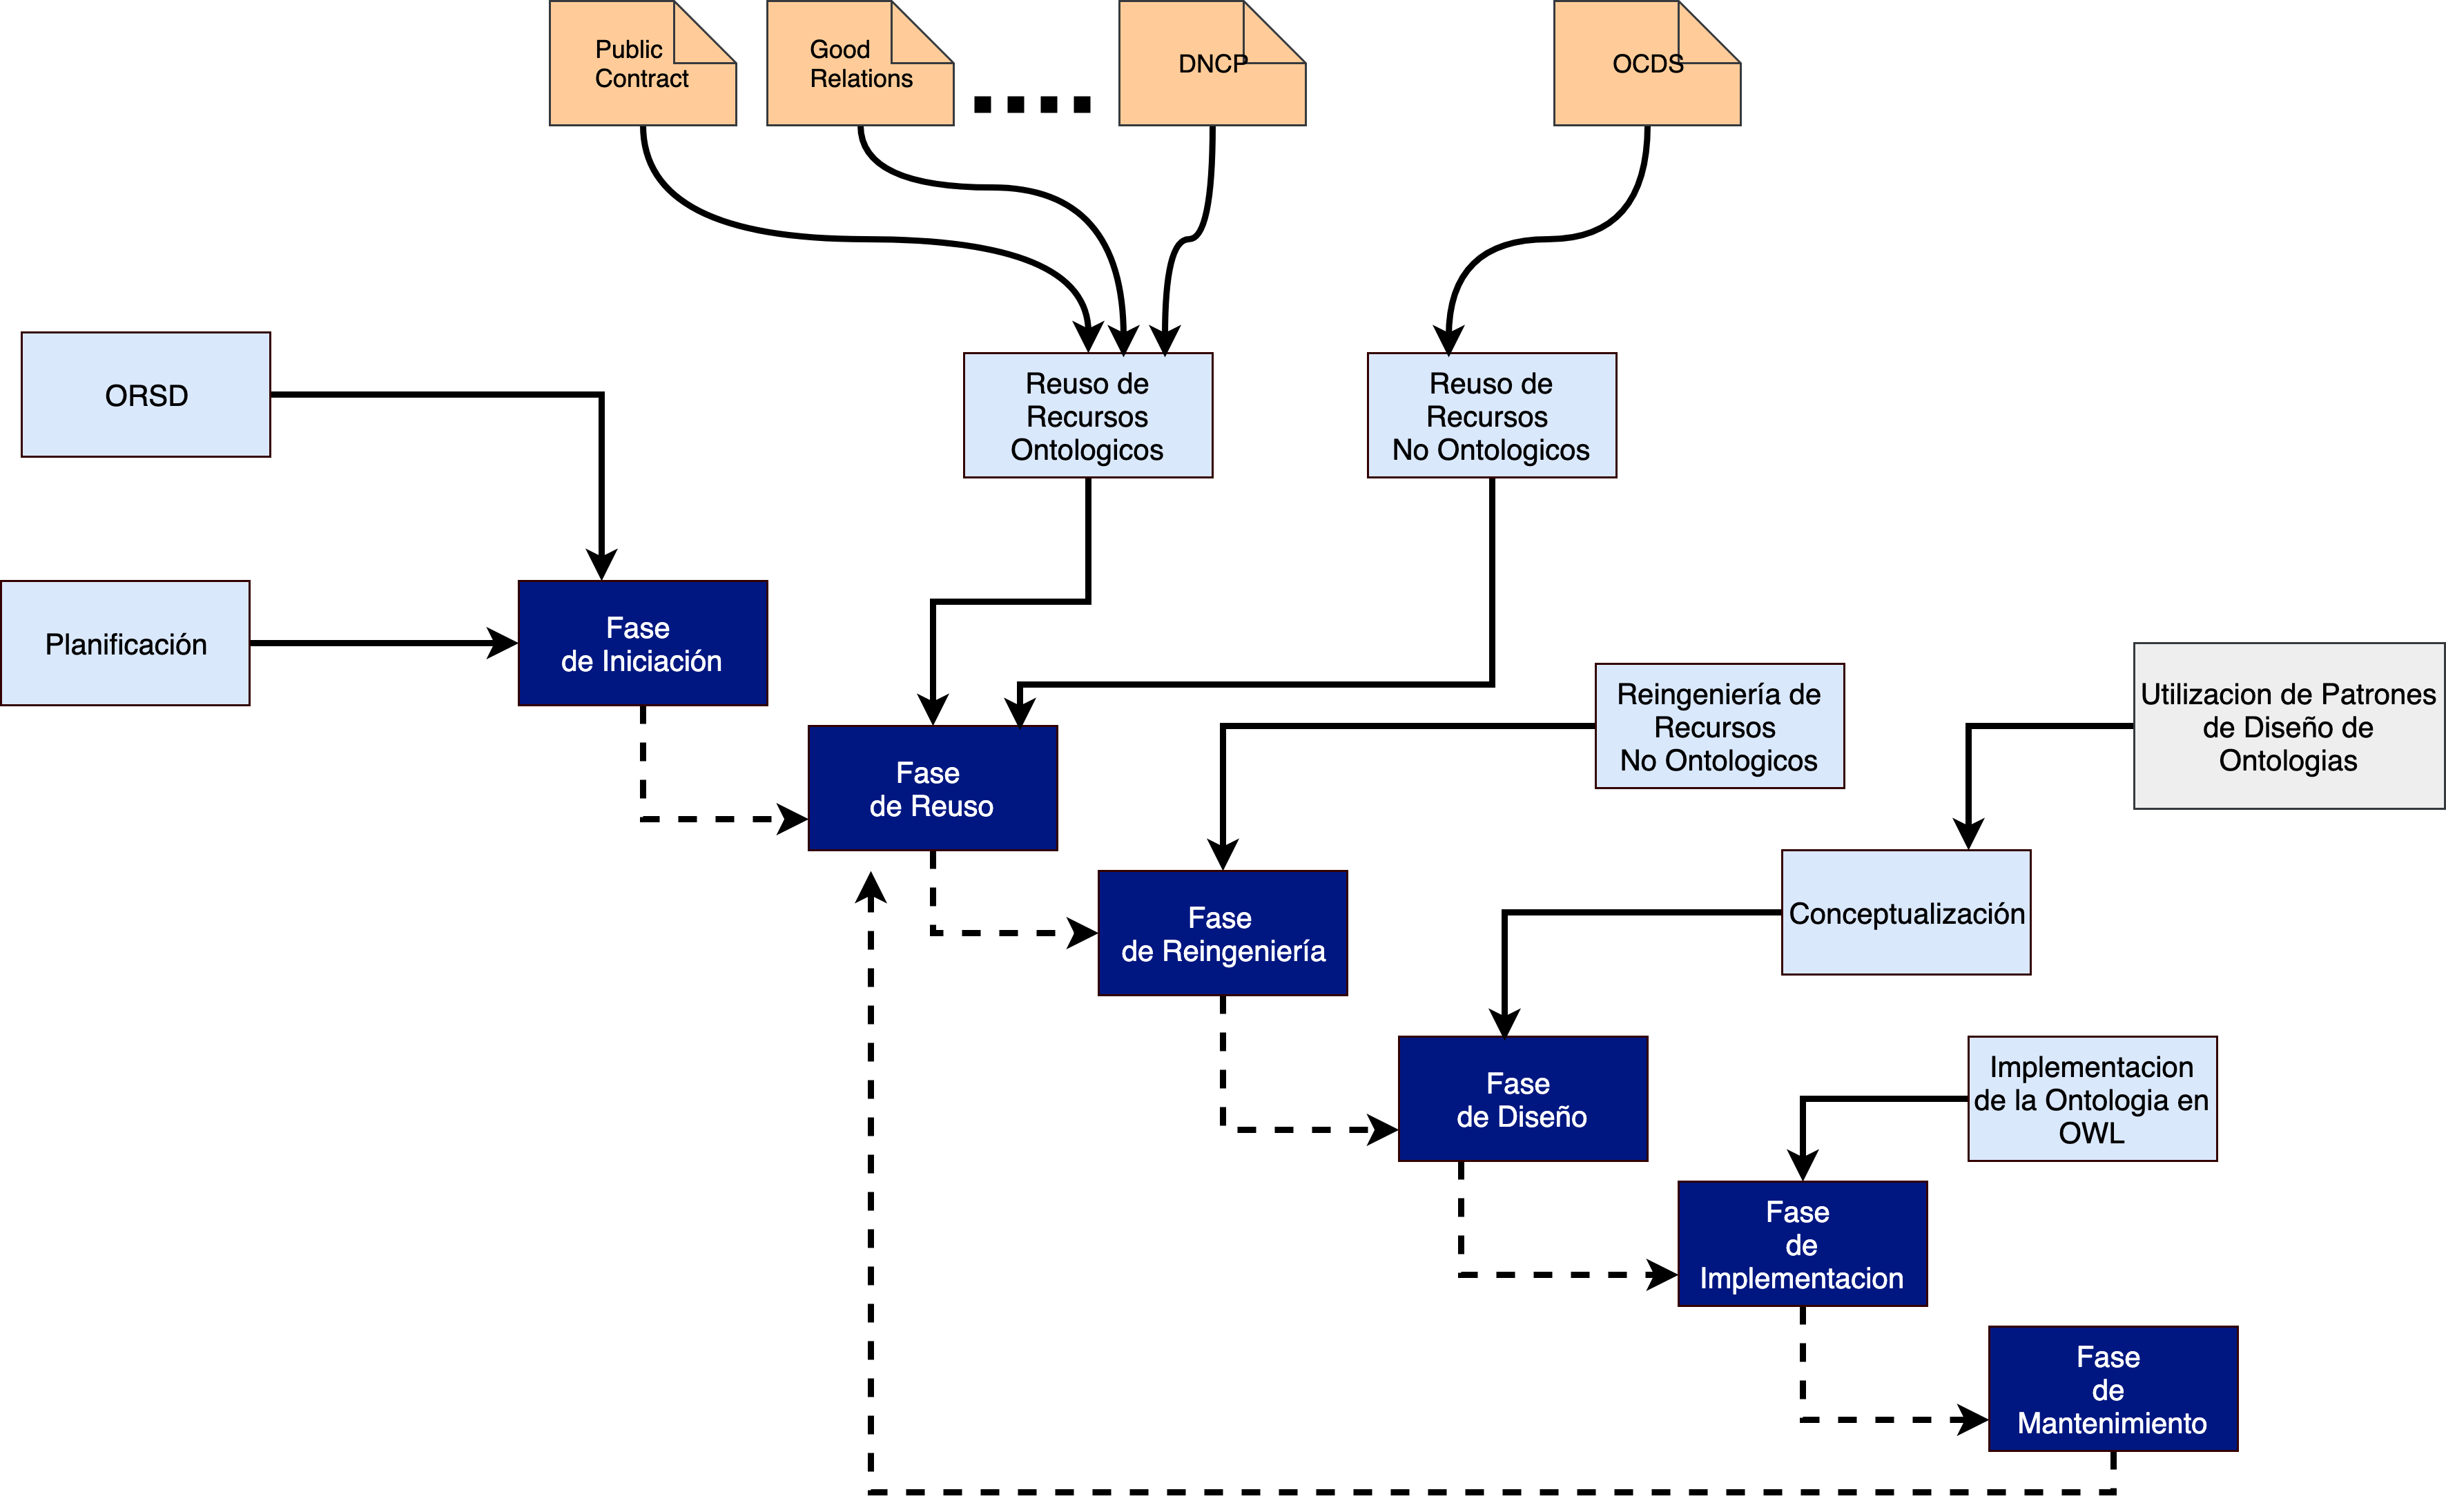
\includegraphics[width=150mm]{figuras/Diagramas-GraficodeSecuenciasDesarrollo.png}
    \caption{Modelo de Ciclo de Vida de desarrollo de la ontología.}
    \label{img:secuenciaDeDesarrollo}
\end{figure}

A continuación se citan las actividades divididas en las fases del ciclo de vida a desarrollarse según la metodología NeOn:
\begin{enumerate}
\item Fase 1: Iniciación
    \begin{enumerate}
    \item Especificación de Requerimientos Ontológicos (ORSD). Aquí se define el propósito de la ontología, su alcance, el lenguaje de implementación, el grupo objetivo, los potenciales usos de la ontología, los requerimientos funcionales y no funcionales, y un pre-glosario de términos.

    \item Planificación. Según lo expuesto en la Tabla \ref{escenarios vs modelo} se elige el modelo de ciclo de vida de 6 fases en cascada, debido a que serán necesarias las fases de reuso tanto de recursos ontológicos como no-ontológicos, reingeniería, y diseño para la implementación.
 
    \end{enumerate}
\item Fase 2: Reuso
    \begin{enumerate}
    \item Reuso de Recursos  no-ontológicos. Los recursos no-ontológicos (NOR) representan recursos de conocimiento cuya semántica no fue formalizada por una ontología. Estos NORs contienen conocimientos de un dominio en particular y representan algún grado de consenso colectivo.

    \item Reuso de Recursos Ontológicos. A fin de no redoblar esfuerzos y con la intención de integrar esta nueva ontología con otras, se procede al reuso de recursos ontológicos. En esta actividad se procedió a la búsqueda, evaluación y selección de las ontologías a reusar.
    \end{enumerate}
\item Fase 3: Reingeniería
\begin{enumerate}
\item Reingeniería de Recursos No-Ontológicos. En esta actividad se analizan posibles patrones de diseño a la hora de la implementación, así como una metodología para transformar la semántica incluida en el OCDS.

\end{enumerate}
\item Fase 4: Diseño
\begin{enumerate}
\item Conceptualización de la Ontología. En esta actividad se identifica el esquema de recursos así como también los componentes conceptuales y sus relaciones. Además, se crea un modelo conceptual dividido por bloques de conceptos relacionados. El conocimiento se expresa mediante representaciones primitivas de conceptos y relaciones entre conceptos. A continuación se representa la conceptualización teniendo como base el OCDS. 

\end{enumerate}
\item Fase 5: Implementación. En esta actividad se procede al desarrollo de la ontología utilizando la herramienta Protégé, el lenguaje utilizado fue OWL, un estándar internacional para codificar e intercambiar ontologías diseñada para la Web Semántica. 

\item Fase 6: Mantenimiento. Por último se procede a la fase del mantenimiento, que consiste en corregir o aumentar los conceptos y restricciones de la ontología para que responda a la preguntas y la detección y corrección de errores de la misma. 		

\end{enumerate}
Una vez terminada la planificación se procede al desarrollo de cada una de las demás actividades siguiendo el orden de las fases. La explicación de cada una de las actividades se describen a continuación en este documento.


\section{Reuso de recursos no-ontológicos}
Los recursos no-ontológicos (NOR)\cite{ReusoRecursoNoOntologico} representan recursos de conocimiento cuya semántica no fue formalizada por una ontología. Estos NORs contienen conocimientos de un dominio en particular y representan algún grado de consenso colectivo. Estos recursos están presentes en forma de esquemas de clasificación, tesauros, diccionarios, etc. El principal desafío de los NORs es que la semántica no siempre está formalizada, osea legible por máquina, por lo tanto no son considerados ontologías formales según la definición adoptada.

En esta sección se desarrolla la búsqueda, evaluación y selección de recursos no-ontológicos que servirán como insumo para el desarrollo de la ontología.

\subsection{Búsqueda de recursos no-ontológicos }

En el proceso de búsqueda de documentación y estándares del dominio de Contrataciones Públicas se encontró que la DNCP implementa una API utilizando el estándar de publicación de datos de contrataciones públicas internacional \textit{Open Contracting Data Standard} (OCDS). La intención de la OCP fue crear un estándar que formaliza la sintaxis y no la semántica de cada concepto, a través de JSON Schema\cite{JSONSche10:online}, que es un vocabulario que permite anotar y validar documentos JSON. El estándar posee conceptos explícitamente definidos en lenguaje natural, por ello se lo consideró un recurso no-ontológico. Cabe recordar que cuando se habla de formal, se habla de legible por máquina. 

OCDS es un estándar amigable y flexible para estructurar información de Contrataciones Públicas y es mantenido por la OCP. El estándar describe qué, cuándo y cómo disponibilizar datos y documentos asociados en las diferentes fases del proceso de contratación. El proyecto promueve la divulgación y participación en las contrataciones públicas creando un estándar abierto de datos simple. OCDS posee un esquema de datos detallado de todos los conceptos así como también la estructura de los datos divulgados, dicho esquema esta disponible el sitio web del estándar \cite{OCDSReleaseSchema:online}. Este esquema ayuda a las personas a comprender todos los campos publicados. Además el estándar posee un guía de implementación de modo a facilitar la implementación de cada país.

Se utilizó el portal de datos abiertos de la DNCP \cite{DatosAbiDNCP:online}, organismo del estado que publica datos de los procesos de contrataciones orientados a diferentes tipos de usuarios:


\begin{enumerate}
    \item Lista de datos. Con el fin de que los usuarios que necesitan ver, analizar y descargar en formato CSV los datos detallados de todos los registros de contrataciones.
    Visualizaciones de datos para usuarios que deseen ver estadísticas e información agregada.
    \item Una API para desarrolladores que permite manipular datos en formato JSON y JSON-LD de manera programática para cualquier otro uso.
    \item Plataforma de Contrataciones Electrónica, destinada a empresas y personas que deseen presentarse o conocer algún proceso de contratación.
\end{enumerate}

Los datos publicados poseen un diccionario de datos y una ontología creada por la DNCP, la cual sirve como contexto para la API desarrollada. Además la DNCP implementó una API siguiendo el estándar OCDS, que posee un esquema de publicación bien definida en JSON Schema.

\subsection{Evaluación de recursos no-ontológicos}
Se eligió el OCDS como recurso no-ontológico a evaluar puesto que el principal objetivo de este trabajo es que la ontología desarrollada sea compatible con dicho estándar de modelo de datos. Para realizar la evaluación se procedió a la extracción de las entradas léxicas, luego al cálculo de precisión y alcance para por último evaluar la factibilidad de reuso del recurso.  A continuación se explica en detalle cada paso.

\subsubsection{Extracción de entradas léxicas}
La meta de esta tarea es extraer las entradas léxicas de los recursos no-ontológicos. Para realizarla, es necesario tomar como entrada los recursos no-ontológicos y extraer sus entradas léxicas usando herramientas de extracción de terminología.	
			
Del esquema JSON de la versión 1 del OCDS se hizo una lista de todas las propiedades del mismo. Para este trabajo consideramos que cada propiedad del esquema consiste en una entrada léxica, donde una entrada léxica corresponde a un concepto o relación dentro del dominio de conocimiento. Se encontraron 142 propiedades, omitiendo las propiedades repetidas y datos transaccionales del estándar que no representan entradas léxicas, la lista se reduce a 114.

\subsubsection{Cálculo de precisión y alcance}

El objetivo de esta tarea es calcular la precisión de los recursos no-ontológicos candidatos. La precisión es una medida ampliamente utilizada en la recuperación de información y se define como la proporción del material recuperado que realmente es relevante. Esta tarea es llevada a cabo por los desarrolladores de software y los que utilicen la ontología teniendo como entrada las entradas léxicas extraídas de los recursos no-ontológicos y de la terminología reunida del ORSD. Para esto definimos los siguientes términos.

\begin{itemize}
    \item \textit{NOR Lexical Entries}  como el conjunto de entradas léxicas extraídas del recurso no ontológico.	
    \item \textit{ORSD Terminology} como el conjunto de términos identificados incluidos en el ORSD. 
\end{itemize}
Para obtener el número de términos de la especificación de requisitos de ontología (ORSDTerminology) se creó una lista unificada de todas las propiedades encontradas en el diccionario de datos del portal de datos abiertos de la DNCP.  Se encontraron 129 términos, de la misma manera que en el OCDS se omitieron propiedades repetidas y datos transaccionales, dejándonos con un total de 109 términos. Éstas representan el dominio de conocimiento que se quiere representar con la ontología a construir.

Para calcular la cobertura y la precisión del recurso no-ontológico se realizó la unión de términos equivalentes semánticamente. Dicha unión consiste en verificar términos equivalentes entre las entradas léxicas que estaban presentes en los requerimientos y en el recurso no-ontológico analizado. Cabe destacar que la metodología utilizada sólo tomó en cuenta las propiedades del esquema JSON del OCDS y el diccionario de datos de la API desarrollada por la DNCP, esto limita la cobertura, que podría ser más amplia si consideramos todos los términos del dominio de conocimiento. El resultado arrojó que existen 65 entradas léxicas comunes. Con estos datos se puede calcular la cobertura y la precisión a través de las  fórmulas \ref{eq:1} y \ref{eq:2}.

\begin{equation}
    \label{eq:1}
    Precision =  \frac{{NORLexicalEntries}*{ORDSTerminology} }{{NORLexicalEntries}}    
\end{equation}

\begin{equation}
    \label{eq:2}
     Coverage = \frac{{NORLexicalEntries}* {ORDSTerminology}}{{ORDSTerminology}}   
\end{equation}

Esto da una cobertura de 0.59 y una precisión de 0.57. 

\subsection{Evaluación y selección del recurso no-ontológico}

Como se puede ver en el esquema del OCDS\footnote{http://standard.open-contracting.org/latest/en/schema/release/}, el mismo posee una especificación formal de la sintaxis de cada una de las propiedades, ya que por medio de un validador construido por la OCP\footnote{http://standard.open-contracting.org/validator/} podemos verificar si el objeto validado cumple con los requerimientos sintácticos de publicación del estándar.

También podemos observar que el estándar contiene explícitamente las descripciones de cada una de las propiedades del esquema JSON, por lo que posee información valiosa y consensuada de cada uno de los conceptos del dominio. Sin embargo, dicha información solamente es entendible por personas, no así procesable por máquinas, por lo que representa un recurso no-ontológico vital para el desarrollo de nuestra ontología.

Como se puede ver en el esquema del OCDS, el mismo posee una especificación formal de la sintaxis de cada una de las propiedades, ya que por medio de un validador construido por la OCP podemos verificar si el objeto validado cumple con los requerimientos sintácticos de publicación del estándar.

También podemos observar que el estándar contiene explícitamente las descripciones de cada una de las propiedades del esquema JSON, por lo que posee información valiosa y consensuada de cada uno de los conceptos del dominio. Sin embargo, dicha información solamente es entendible por personas, no así procesable por máquinas, por lo que representa un recurso no-ontológico vital para el desarrollo de nuestra ontología.



Las principales diferencias de cobertura entre los conceptos de la DNCP y la OCDS son que el segundo posee mayor información como es el caso de Periodo, Organización y Detalle de Contacto. También contempla los conceptos de Documentos, Transacciones, Hitos, una fase adicional de Implementación del Contrato y guarda el historial de cambios de todas las propiedades a través de las Adendas. Así también, el dominio de la DNCP agrega conceptos como Modificaciones de Contrato e información más detallada de Proveedores y Convocatorias. En la figura \ref{img:coberturaontologia} se aprecia la intersección de los principales conceptos entre ambos dominios de conocimientos.

\begin{figure}[ht!]
    \centering
    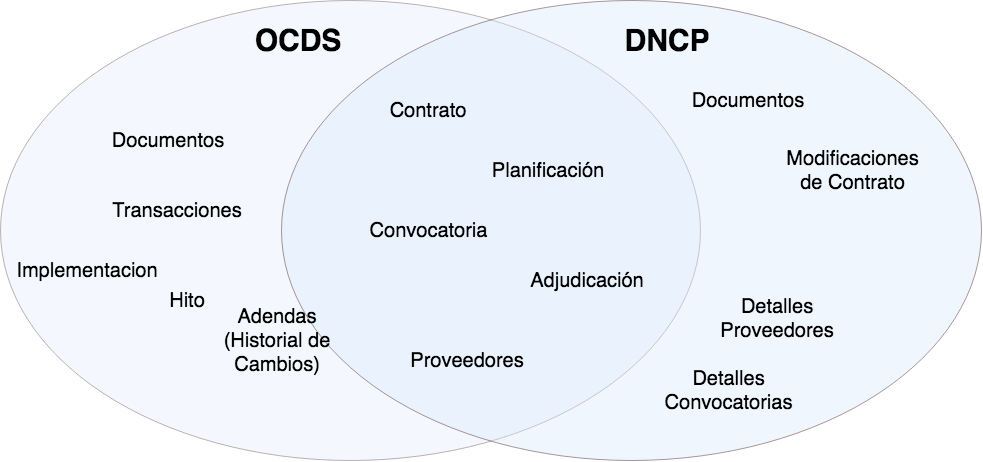
\includegraphics[width=150mm]{figuras/Diagramas-VennCobertura.png}
    \caption{Cobertura de los terminos de la DNCP y la OCDS}
    \label{img:coberturaontologia}
\end{figure}

    

El OCDS es implementado a nivel internacional, tiene una comunidad de colaboradores expertos en el dominio de distintos países, implementadores que dan al estándar una validez en cuanto a la aceptación de los términos, posee listas de correos y un sistema de gestión de cambios y mejoras activo en la plataforma Github\footnote{https://github.com/open-contracting/standard}. La intención de este trabajo es que la ontología sea utilizada no solamente sea utilizada por la DNCP sino por cualquier ente que realice procesos licitatorios, además, la DNCP está utilizando este estándar para publicación de datos orientados a desarrolladores. Con todo esto se aprecia que la cobertura es suficiente para utilizar el OCDS como recurso no-ontológico para nuestra ontología sacrificando así algunos detalles específicos de implementación local. Estos detalles más específicos se podrían cubrir a través del reuso y extensión de la ontología desarrollada en un futuro trabajo.

\section{Reingeniería de recurso no-ontológicos}
Debido a que se utilizó recursos no-ontológicos, debemos de realizar un proceso de reingeniería para transformar estos recursos de manera a incluir esa información en la ontología. Procedemos de esta manera al proceso de reingeniería del esquema de publicación de OCDS.


\subsection{Ingeniería reversa del recurso no-ontológico}
El primer paso es analizar el recurso no-ontológico para identificar los principales componentes y crear representaciones del recurso. Dentro de esta actividad procederemos a la recolección de los datos, la abstracción conceptual y exploración de la información.

\subsubsection{Recolección de datos}

El propósito de esta actividad es buscar y recolectar todos los datos y la documentación del recurso no-ontológico incluyendo su propósito, componentes, modelo de datos y detalles de implementación.

El OCDS es un estándar abierto de datos para la publicación de información estructurada sobre todas las etapas de un proceso de contratación: desde la planificación hasta la implementación.

La publicación de los datos siguiendo el OCDS permite una mayor transparencia en la contratación pública y puede apoyar al análisis accesible y a profundidad de la eficiencia, efectividad, equidad e integridad de los sistemas de contratación pública. El OCDS fue diseñado con un enfoque en la contratación pública de bienes, obras y servicios, pero puede ampliarse para su uso en otros contextos. 

El OCDS se centra en las siguientes necesidades del usuario:
\begin{itemize}
    \item Fortalecimiento de la transparencia, rendición de cuentas e integridad de los contratos públicos.
    \item Hacer un buen uso del dinero del gobierno.
    \item Permitir al sector privado una competencia justa por contratos públicos.
    \item Control de la eficacia de la prestación de servicios. 
\end{itemize}

El OCDS posee un sitio web donde se encuentra documentado todo el estándar, soportando los idiomas español, inglés y francés. Además posee una guía de implementación del estándar, un validador de la estructura sintáctica del mismo y un mecanismo de gestión de extensiones.

\subsubsection{Modelo conceptual}

En esta actividad se identifica el esquema de recursos así como también los componentes conceptuales y sus relaciones. Además se crea un modelo conceptual dividido por bloques de conceptos relacionados. El conocimiento se expresa mediante representaciones primitivas de conceptos y relaciones entre conceptos. A continuación se representa la conceptualización teniendo como base el OCDS.

Un proceso de contratación se define como toda la información relativa a la planificación, la licitación, las adjudicaciones, los contratos y la ejecución de contratos relacionados con un solo proceso de iniciación.

Un proceso de contratación agrupa información sobre diferentes etapas o fases relacionadas a la vida útil de un contrato, a partir de la planificación, progresando a través de las etapas de iniciación u oferta, luego por la adjudicación y contrato y finalizando con la implementación del producto o servicio como se muestra en la Figura \ref{img:fases del proceso licitatorio }.

\begin{figure}[!htbp]
    \centering
    
\includegraphics[width=150mm]{figuras/Diagramas_ProcesoLicitatorio.png}
    \caption{Modelo de fases del Proceso Licitatorio}
    \label{img:fases del proceso licitatorio }
\end{figure}

Las etapas son correlativas, esto significa que necesariamente debe de existir la etapa anterior antes de existir la siguiente. Todas las etapas representan un bloque de información.

Además de estas etapas existe otro concepto importante que es el bloque de Organización, que puede corresponder tanto al comprador como al oferente. Esta Organización puede estar ligada a cualquiera de las etapas del proceso de contratación. A continuación se detallan cada una de las etapas.
\paragraph{Planificación (\textit{Planning})}\hfill \break
Este bloque contiene información necesaria para describir los antecedentes de un proceso de contratación y puede incluir detalles del presupuesto del que se extraen los fondos o proyectos relacionados. Todo proceso de contratación posee una única planificación, dicha planificación tiene un presupuesto (budget) asociado donde finalmente se indica el valor o monto estimado para la adquisición del bien o servicio. Un diagrama de los componentes principales de la clase Planificación puede verse en la Figura \ref{img:Fase de Planificacion}.

\begin{figure}[htbp!]
    \centering
    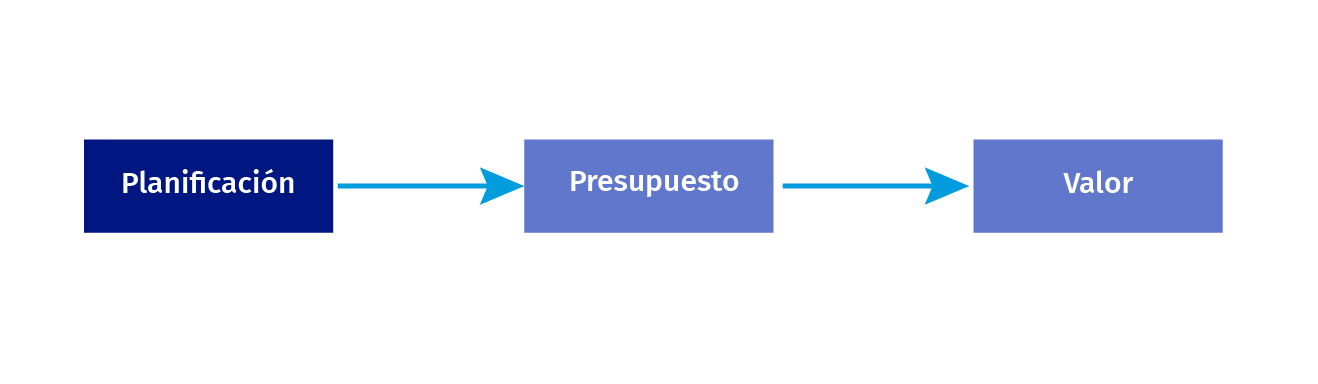
\includegraphics[width=150mm]{figuras/Diagramas_Planificacion.png}
    \caption{Modelo de fase de Planificación}
    \label{img:Fase de Planificacion}
\end{figure}

\paragraph{Convocatoria (\textit{Tender})}\hfill \break
Este bloque incluye detalles del anuncio indicando que una organización tiene la intención de abastecerse de algunos bienes o servicios y establecer uno o más contratos para estos. Todo proceso de contratación posee una única convocatoria, dicha convocatoria tiene asociada la organización involucrada en el proceso. Además, la convocatoria indica los ítems requeridos, el período establecido, los documentos utilizados, las adendas que pudieran haberse realizado sobre la convocatoria original y la lista de hitos. Se observa el esquema en la Figura \ref{img:Fase de Convocatoria}

\begin{figure}[htbp!]
    \centering
    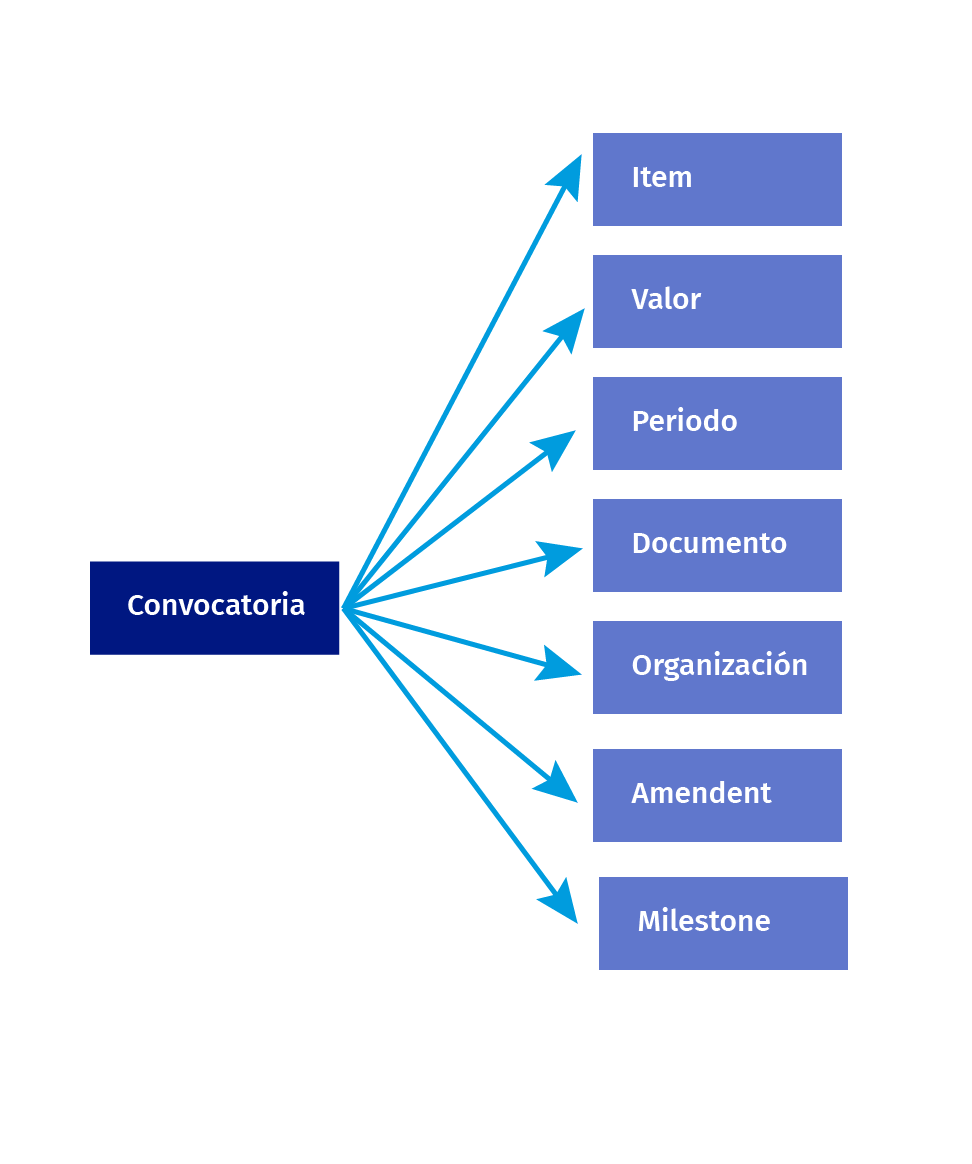
\includegraphics[width=150mm]{figuras/Diagramas_Convocatoria.png}
    \caption{Modelo de fase de Convocatoria}
    \label{img:Fase de Convocatoria}
\end{figure}

\paragraph{Adjudicación (\textit{Award})}\hfill \break
Este bloque se utiliza para anunciar las adjudicaciones emitidas para una licitación. Todo proceso de contratación puede involucrar una o más adjudicaciones, dichas adjudicaciones indican, para cada proveedor (organización), los ítems adjudicados, el valor o monto adjudicado y los documentos asociados al proceso. Esto se aprecia en la Figura \ref{img:Fase de Adjudiacion}


\begin{figure}[htbp!]
    \centering
    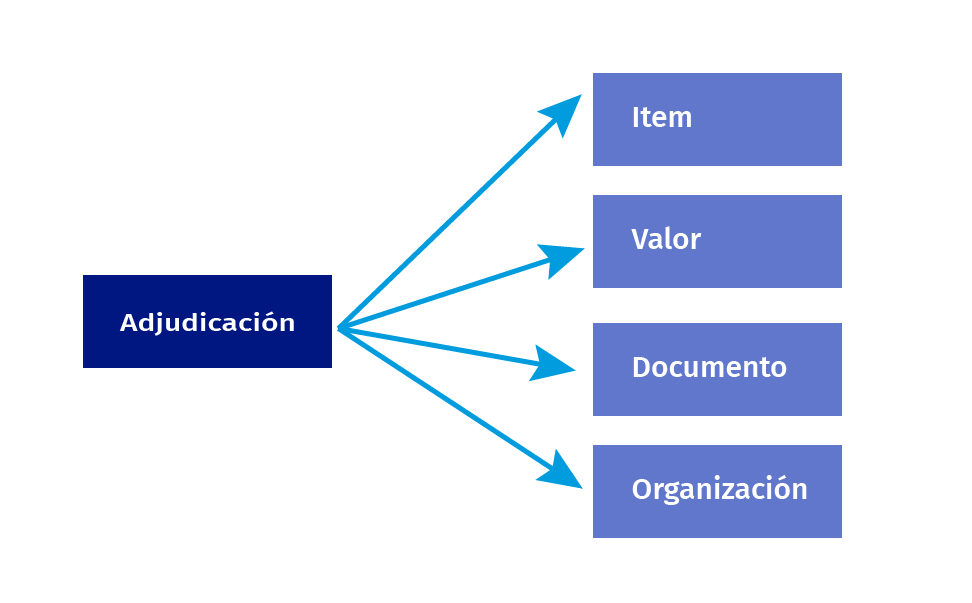
\includegraphics[width=150mm]{figuras/Diagramas_Adjudicacion.png}.
    \caption{Modelo de fase de Adjudicación}
    \label{img:Fase de Adjudiacion}
\end{figure}


\paragraph{Contrato (\textit{Contract})}\hfill \break
Este bloque se utiliza para proporcionar detalles de los contratos que se han celebrado. Todo proceso de contratación puede involucrar uno o más contratos, cada uno de los cuales debe estar asociado a una adjudicación específica. El proveedor (organización) adjudicado está indicado en la adjudicación, no así en el contrato. El contrato también indica los ítems adjudicados, los documentos asociados al proceso y la implementación del contrato. La implementación del contrato contiene información acerca de los hitos, las transacciones realizadas y los documentos utilizados. En la Figura \ref{img:Fase de Contrato} vemos un esquema de la estructura del Contrato.

\begin{figure}[htbp!]
    \centering
    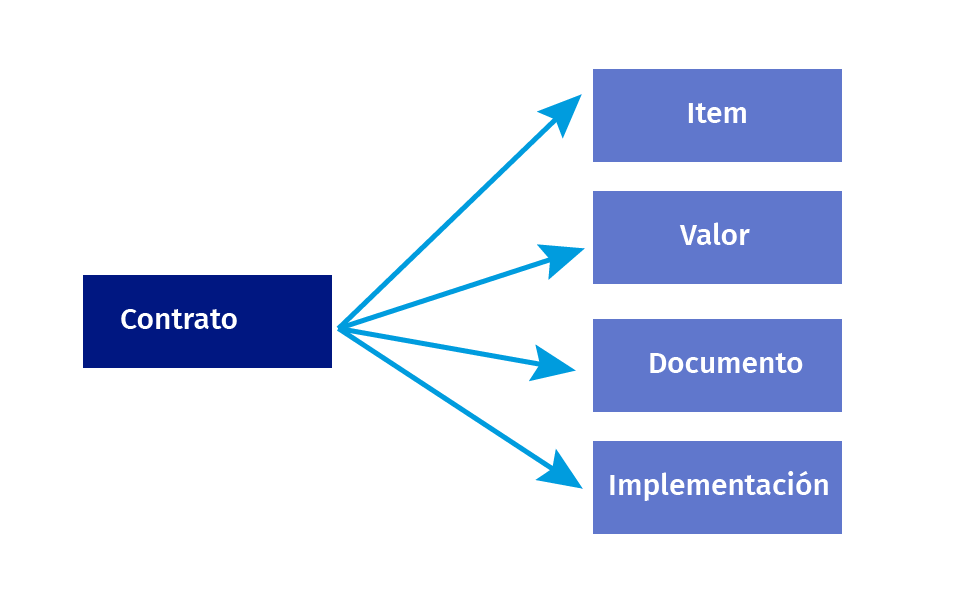
\includegraphics[width=150mm]{figuras/Diagramas_Contrato.png}
    \caption{Modelo de fase de Contrato}
    \label{img:Fase de Contrato}
\end{figure}

\paragraph{Otros componentes del estándar}\hfill \break
El estándar posee además otros componentes o bloques que agrupan y contienen metadatos de publicación de los datos.  A continuación se detallan dichos componentes.

\paragraph{\textit{Releases}}\hfill \break
Para fomentar la mayor apertura de información el estándar está preparado para publicar la información en tiempo real. En cada etapa del proceso de contratación o con cada cambio que ocurra sobre los datos, el estándar prevé la publicación de esa nueva porción de información mediante releases.
Los releases son acumulativos, es decir, durante un proceso de contratación se pueden proporcionar uno o más releases, por ejemplo: describir una licitación, anunciar la adjudicación de contratos y proporcionar actualizaciones sobre los mismos.
Una vez que un release ha sido publicado no puede cambiar. La información actualizada debe ser compartida a través de un nuevo release.
Los releases pueden ser publicados a través de un único sistema o de manera distribuida por diferentes sistemas, pero todos éstos deben estar relacionados a partir de un identificador único denominado Open Contracting ID (OCID).

\paragraph{\textit{Releases}}\hfill \break
Un registro (\textit{Record}) de contratación provee una instantánea del proceso de contratación en un punto dado en el tiempo, que reúne todas las versiones por las cuales pasó ese proceso en un solo lugar.
Un Record contiene tres elementos clave: 
\begin{itemize}
    \item Una lista de todos los releases asociados a un proceso de contratación en particular, 
    \item Un release compilado que contiene la última versión de los datos,
    \item Una versión histórica de releases que contiene la historia con todos los cambios realizados sobre los datos.
\end{itemize}

\paragraph{\textit{Release package}}\hfill \break
Un release package es un esquema de agrupación para la publicación de releases, describe el documento contenedor y metadatos para la publicación de releases.

\paragraph{\textit{Record package}}\hfill \break
Un Record Package es un esquema de agrupación para la publicación de Records, describe el documento contenedor y metadatos para la publicación de Records. En la Figura \ref{img:Record Package} se muestra el modelo conceptual de \textit{Record Package}.



\begin{figure}[ht!]
    \centering
    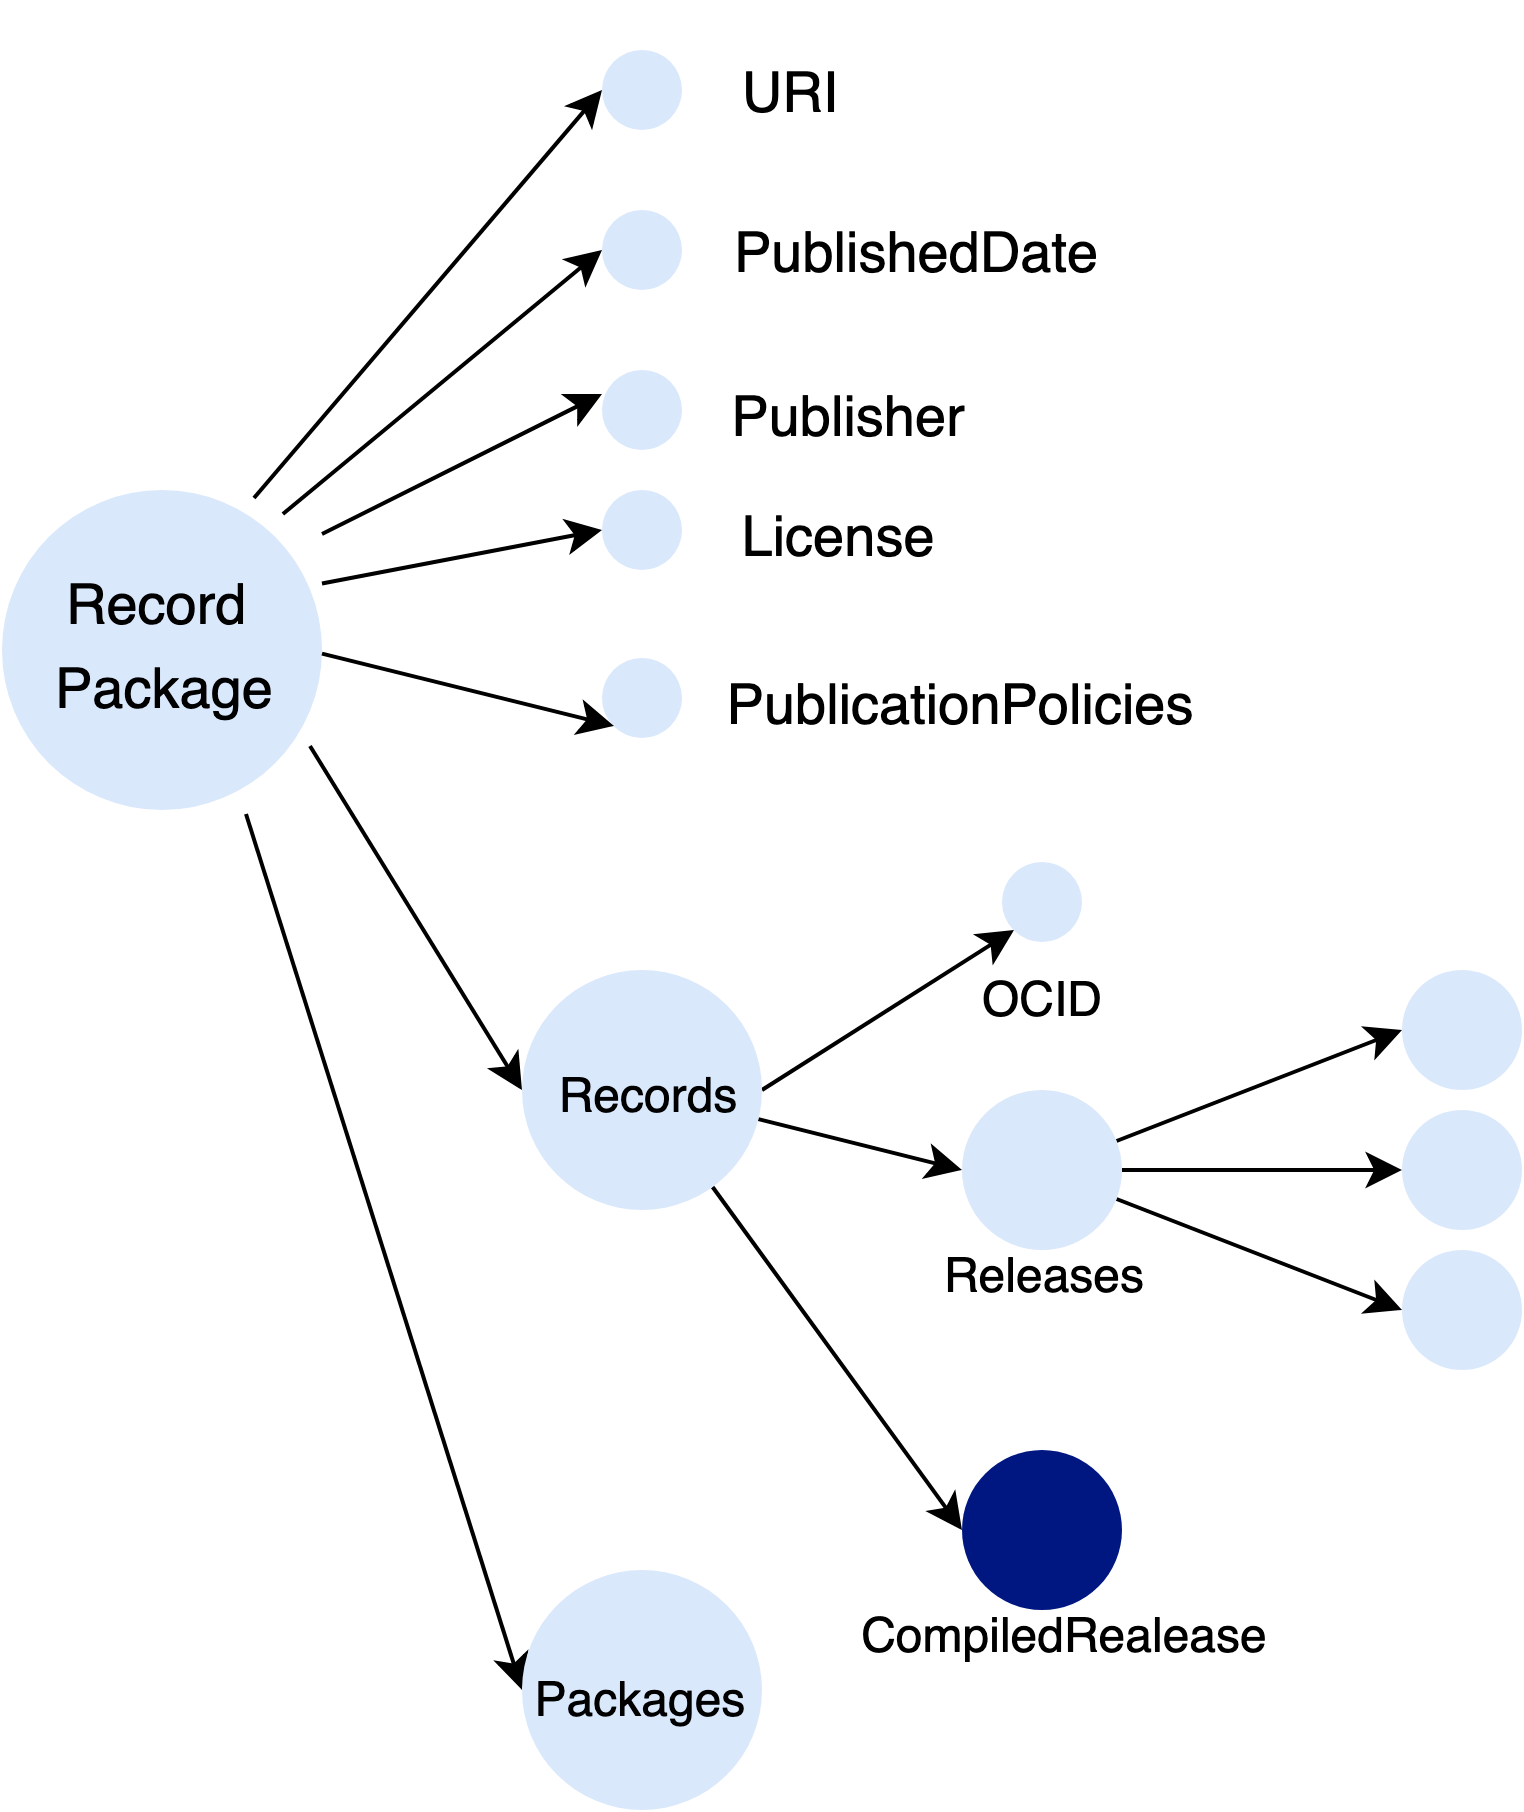
\includegraphics[width=150mm]{figuras/Diagramas-RecordPackage.png}
    \caption{Record Package}
    \label{img:Record Package}
\end{figure}


\subsubsection{Transformación del recurso no-ontológico}
En esta sección se utilizaron los patrones de diseño para seguir construyendo un modelo conceptual y luego proseguir con la implementación de la ontología. 
\paragraph{Búsqueda de Patrones de Diseño}\hfill \break
El objetivo de este paso es buscar posibles patrones de diseño que conviertan el recurso no-ontológico en un modelo conceptual. 
Una vez analizado el esquema del OCDS se procedió a la búsqueda de patrones de diseño de ontologías, se utilizó el repositorio ontologydesingpatterns.org para realizar esta búsqueda de patrones bien conocidos por la comunidad de desarrolladores de ontologías y recomendado por la metodología NeOn.
Los patrones que son relevantes son aquellos que involucran tiempo, dinero, empresas u organizaciones, lugares y procesos en general. Luego de una búsqueda se encontraron los siguientes patrones de diseño que podrían ser útiles al momento del desarrollo de la ontología.
\begin{enumerate}
    \item Intervalo de tiempo\footnote{http://ontologydesignpatterns.org/wiki/Submissions:TimeInterval}
    \item Precio\footnote{http://ontologydesignpatterns.org/wiki/Submissions:Price} 
    \item Etiquetas\footnote{http://ontologydesignpatterns.org/wiki/Submissions:Tagging}
    \item Lugar\footnote{http://ontologydesignpatterns.org/wiki/Submissions:Place}
    \item Lista\footnote{http://ontologydesignpatterns.org/wiki/Submissions:List}
    \item Secuencia\footnote{http://ontologydesignpatterns.org/wiki/Submissions:Sequence}
    \item Boleta de Pago\footnote{http://ontologydesignpatterns.org/wiki/Submissions:Invoice} 
\end{enumerate}

Además se investigaron otros patrones de reingeniería, pero ninguno de éstos se adecuaba ya que están orientados a patrones jerárquicos de diseño y el dominio modela una secuencia o proceso. 

Se creó un patrón de conversión del estándar de documentacion JSON SCHEMA http://json-schema.org/ a un modelo ontológico. El patrón de conversión tiene los siguientes lineamientos.

\begin{itemize}
    \item Todos los objetos JSON del esquema son potenciales conceptos de la ontología desarrollada. Un Objeto JSON será considerado como clase o individuo en el modelo conceptual.
    \item El hecho de que un objeto esté relacionado a otro no necesariamente indica una relación de jerarquía, puede a la vez tratarse de una relación de contención, uso, correlación o dependencia.
    \item Todos los atributos de un Objeto JSON de tipo \textit{string} o numérico son potenciales propiedades (en la ontología) del concepto generado a partir el Objeto JSON.
    \item Los tipos de datos nos indican el tipo de dato en el formato RDF. Por ejemplo, si dentro de JSON Schema tenemos un campo que solo acepta números, podemos decir que esa propiedad es de tipo \textit{xsd:long}. Así, pueden ser una restricción en los valores de la propiedad.
    \item El nombre del objeto JSON es un candidato para nombrar esta relación. Por ejemplo, un presupuesto posee un objeto de nombre monto, de tipo valor. Por lo que podemos decir que el nombre de la relación entre presupuesto y valor se llamará monto.
    \item Los arreglos son representados a través de la relación uno a muchos dentro del modelo ontológico.
    \item Los atributos \textit{id}, \textit{identifier} o similares son potenciales identificadores de las instancias de cada concepto.
    
\end{itemize}

El esquema del OCDS posee una lista de códigos (\textit{Codelist}) de dos tipos, abiertos y cerrados. Los \textit{Codelist} Abiertos proveen códigos sugeridos, los publicadores pueden extender esta lista con nuevos códigos sin el consenso de otros publicadores. Mientras que los \textit{Codelist} Cerrados proveen códigos mandatorios, los publicadores solo pueden utilizar los valores de la lista oficial, cambios a \textit{Codelist} cerrados deben hacerse a través de la gobernanza y revisión de la lista. Esta lista de códigos fueron transformados utilizando el patrón mencionado a continuación. 

Para los \textit{Codelist} Abiertos se los convirtió en \textit{individuals}, en otros términos, instancias de los conceptos. Para los \textit{Codelist} Cerrados  se los convirtió en \textit{Enumerated Classes}. Las \textit{Enumerated Classes} impiden la declaración de nuevos individuos que pertenecen a esta clase, siendo así más restrictivos.
\paragraph{Utilización de patrones}\hfill \break
Por último, se consideraron los patrones mencionados anteriormente para los siguientes conceptos:
Para el concepto \textit{Value} del OCDS, que representan valores monetarios, se utilizó el patrón \textit{Price}. El patrón describe el precio de alguna entidad, dicho precio contiene un valor y una moneda. En la Figura \ref{img:Modelo de Precio} se muestra el diagrama del patrón.

\begin{figure}[ht!]
    \centering
    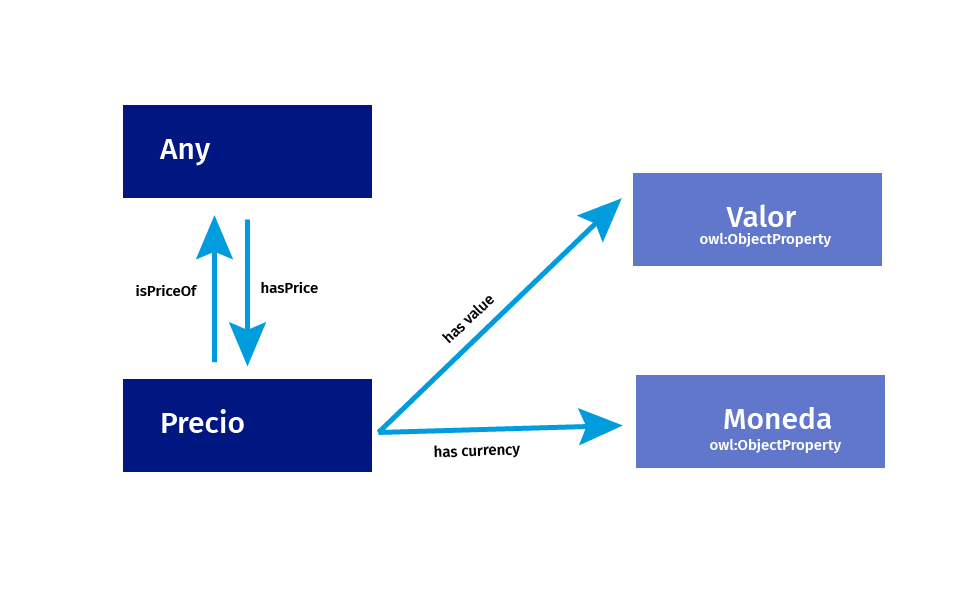
\includegraphics[width=150mm]{figuras/Diagramas_Precio.png}
    \caption{Modelo de Precio}
    \label{img:Modelo de Precio}
    
\end{figure}

En cuanto a la implementación, se optó por mantener \textit{Value} y \textit{Currency} como \textit{DataType properties} para mantener la simplicidad de nuestra ontología.

Para el concepto \textit{Period}, que representan periodos de tiempo se utilizó el patrón \textsc{Time Interval}. El patrón describe un intervalo de tiempo que contiene una fecha de inicio, una fecha de fin y una fecha del intervalo. Un posible uso del patrón sería la fecha “Agosto del 2018” tiene un fecha de inicio “1 de Agosto” y una fecha de fin “31 de Agosto”. En la implementación se omitió la propiedad Intervalo de tiempo, ya que no es necesaria para este este dominio. El modelo se puede ver en la Figura \ref{img:Modelo de Intervalo de precio}.

\begin{figure}[ht!]
    \centering
    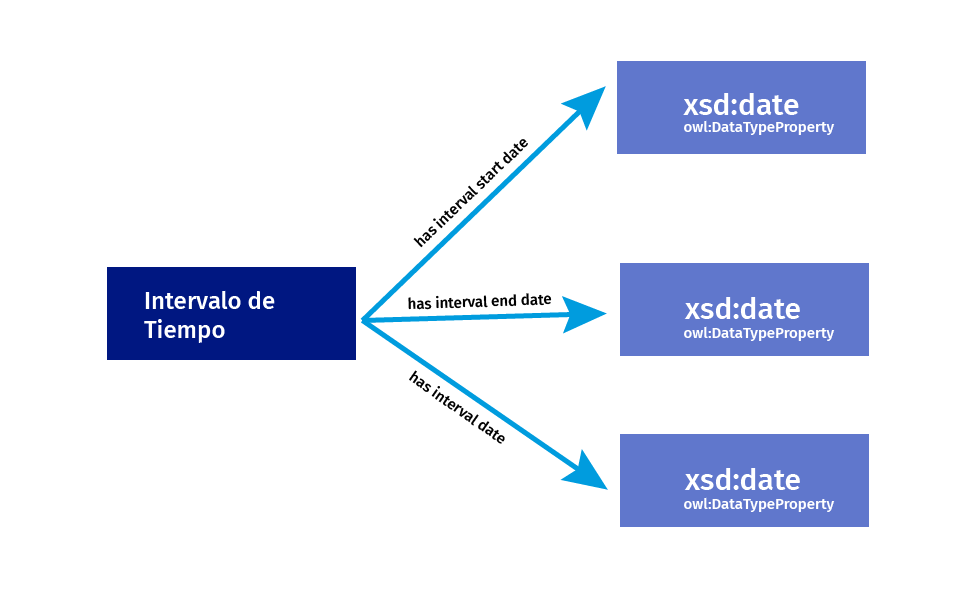
\includegraphics[width=150mm]{figuras/Diagramas_Tiempo.png}
    \caption{Modelo de Intervalo de tiempo}
    \label{img:Modelo de Intervalo de precio}
    
\end{figure}

Para la relación que existe entre \textit{Planning, Tender, Award, Contract e Implementation}, que tienen una relación de dependencia y de secuencia, se utilizó el patrón \textit{Sequence}. El patrón describe una secuencia de hecho a través de las propiedades Precede, Precede Directamente, Antecede y Antecede Directamente. Por ejemplo, decidir qué camisa utilizaré precede directamente a colocarse la camisa, y precede a colocarse la corbata. En la Figura \ref{img:Modelo de dependencia y secuencia} se presenta el diagrama del patrón. Se utilizó este patrón para describir la secuencia del proceso de contrataciones.

\begin{figure}[ht!]
    \centering
    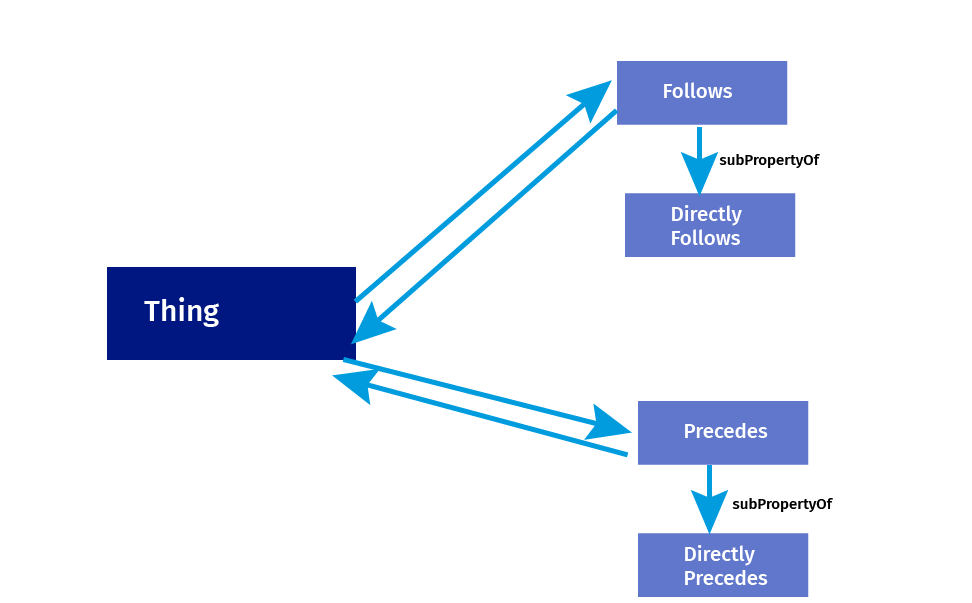
\includegraphics[width=150mm]{figuras/Diagramas_Follows.png}
    \caption{Modelo de dependencia y secuencia}
    \label{img:Modelo de dependencia y secuencia}
    
\end{figure}

\subsubsection{Construcción de la ontología}

Una vez concluido el modelo conceptual de la ontología procedemos a la construcción de la misma utilizando el lenguaje OWL y la herramienta Protégé.

Dentro de la fase de búsqueda de recursos Ontológicos, se encontró una ontología desarrolladas\footnote{https://github.com/ColinMaudry/open-contracting-ld} por un colaborador al proyecto OCD, la ontología siguió una transformación directa de JSON SCHEMA del estándar, la misma representa un punto de partida para seguir desarrollando la ontología. De esta manera además queremos incentivar la colaboración y hacer partícipe a toda la comunidad del OCDS.

El primer paso fue importar la ontología al software Protégé. Al hacer esto el software reestructuró el código de la ontología e hizo inferencias básicas detalladas a continuación. La estructura del documento del cual se partió estaba agrupada según conceptos semánticos relacionados. Protégé estructuró la ontología según sean \textit{Annotation Property, DataType Property u Object property} y luego ordenó de forma alfabética tomando como referencia el nombre de la propiedad.

Se encontraron algunas inconsistencias sintácticas dentro de la ontología, debido a que la misma fue hecha sin utilizar ninguna herramienta para desarrollo de ontologías, lo cual da lugar a errores sintácticos. Por ejemplo, el rango de la clase \textit{FormerValue} estaba definido como \textit{xsd:Integer}, Protégé infiere de que se trataba de un nuevo tipo de dato,  debido a que no existe este tipo de dato sino que debe ser \textit{xsd:integer}. Así también otro error en el documento en donde se escribió \textit{commnent} en lugar de \textit{commnent}, inmediatamente Protégé infiere como un nuevo tipo de dato. Como aprendizaje, el uso de una herramienta ontológica como Protégé nos ayuda a prevenir errores de sintaxis en la creación de la ontología y además acelera el proceso de desarrollo gracias a una interfaz gráfica que nos ayuda a distinguir entre Clases, \textit{DataType Properties} por citar algunas funcionalidades.

Toda la ontología inicial utilizó el tipo \textit{rdf:Property} para definir las propiedades. Debido a que \textit{owl:ObjectProperty} y \textit{owl:DataTypeProperty} son subclases de \textit{Property}, se decidió especializar las relaciones con estas subclases. Las propiedades que relacionan dos instancias fueron asignadas como owl:ObjectProperty y las propiedades relacionadas entre una instancia y un valor fueron asignadas como owl:DataTypeProperty.

Una propiedad de objeto (\textit{ObjectProperty}) se utiliza para conectar pares de individuos a través de IRIs, mientras que una propiedad de tipo de dato (\textit{DataTypeProperty}) relaciona una instancia de una clase con un literal.

Una propiedad funcional (\textit{FunctionalProperty}) es una propiedad que solamente puede tener un valor Y por cada instancia X, por ejemplo no puede haber dos valores distintos Y1 e Y2 tal que los pares (X,Y1) y (X,Y2) sean instancias de esta propiedad. Tanto los “ObjectProperty” como los \textit{DataTypeProperty} pueden ser declarados como \textit{DataTypeProperty}.


Una consideración importante es que para los \textit{DataType Properties} no es necesario definir como la propiedad functional ya que la mayoría de los motores de razonamiento pueden deducir que dos literales son distintos. Ejemplo: un razonador puede inferir que  el literal “1” es distinto que  "2".

El motor de inferencia agregó un axioma indicando que rdf:descriptions es igual a \textit{owl:AnnotationProperty}, que es una manera de anotar información descriptiva de la propiedad. Además se utilizó la propiedad \textit{rdf:Resource}, clase que no existe en en el estándar RDF, debería indicar la clase RDFS \textit{ rdfs:Resource} para indicar hipervínculos. En este caso se vió que semánticamente se adecua mejor la propiedad \textit{DCTERMS:URI}.

Así, se pudo construir la ontología base partir de un recurso No-Ontológico como ser el Open Contracting Data Estándar. En el siguiente apartado se abocará a la búsqueda y reutilización de recursos Ontológicos para enriquecer la ontología desarrollada.


\section{Reuso de Recursos Ontológicos}
Los pasos para el reuso de una ontología son la búsqueda, análisis y comparación de ontologías desarrolladas y luego la selección e integración de las ontologías a reutilizar. Al mismo tiempo existen distintas maneras de reutilizar una ontología, como veremos más adelante. 

\subsection{Búsqueda de Ontologías}
\label{section:busqueda de ontologias}

Un parámetro importante a la hora de hacerlo es la cantidad de veces que esta ya fue reutilizada. \textit{Linked Open Vocabularies}(LOV) es un repositorio de ontologías bien curado y estable mantenido por la \textit{Open Knowledge Foundation}  (OKF) que nos muestra la cantidad de conexiones entre las ontologías.

\subsubsection{Ontologías Relacionadas}

Con relación a ontologías más generales y relacionadas de alguna manera al dominio que pudieran ayudar a enriquecer las ontologías desarrolladas se encontraron las siguientes:
\begin{itemize}
    \item \textit{Organization}\cite{TheOrgan48:online} : Ontología central para las estructuras de una organización, destinada a apoyar la publicación de datos vinculados de la información de la organización en una serie de dominios. Está diseñada para permitir extensiones específicas de dominio para agregar clasificación de organizaciones y roles, así como extensiones para admitir información relacionada, como actividades de la organización.
    \item \textit{Good Relations}\cite{hepp2008goodrelations} : es un vocabulario estandarizado para datos de productos, precios, tiendas y empresas que pueden integrarse en páginas web estáticas y dinámicas existentes y eso puede ser procesado por otras computadoras. Esto aumenta la visibilidad de sus productos y servicios en la última generación de motores de búsqueda, sistemas de recomendación y otras aplicaciones novedosas.
    \item \textit{DCTERMS}\cite{DCMIDCMI37:online}: Una especificación actualizada de todos los términos de metadatos mantenidos por la Dublin Core Metadata Initiative, que incluye propiedades, esquemas de codificación de vocabulario, esquemas de codificación de sintaxis y clases. 
\end{itemize}

\subsubsection{Ontologías del dominio de Contrataciones Públicas.}

Observando LOV dentro del dominio de estudio, se realizó una búsqueda a través de la etiqueta “Contract”, teniendo como resultado los siguientes recursos ontológicos:

\begin{enumerate}
    \item c4n - Call for Anything vocabulary \footnote{https://lov.linkeddata.es/dataset/lov/vocabs/c4n}
    \item eli- The European Legislation Identifier \footnote{https://lov.linkeddata.es/dataset/lov/vocabs/eli}
    \item ldr - Linked Data Rights \footnote{https://lov.linkeddata.es/dataset/lov/vocabs/ldr}
    \item loted - LOTED ontology \footnote{https://lov.linkeddata.es/dataset/lov/vocabs/loted}
    \item pay - Payments ontology \footnote{https://lov.linkeddata.es/dataset/lov/vocabs/pay}
    \item  pc - Public Contracts Ontology \footnote{https://lov.linkeddata.es/dataset/lov/vocabs/pc}
    \item pproc - PPROC ontology \footnote{https://lov.linkeddata.es/dataset/lov/vocabs/pproc} 
    \item LOTED 2 - LOTED ontology 2 \cite{distinto2014loted2}
    \item DNCP - Ontologia desarrollada por la DNCP \footnote{https://www.contrataciones.gov.py/datos/def/dncp.owl}
\end{enumerate}


Haciendo una búsqueda más exhaustiva dentro del dominio de contrataciones públicas a través de internet se pudo identificar también las ontologías LOTED 2 y la ontología desarrollada por la DNCP.

En este trabajo se pone bajo análisis las ontologías de LOTED 2 , LOTED, Public Contract y PPROC, esta última es la más reciente y en su desarrollo se tomó en cuenta la experiencia de las primeras. Por último también se pone bajo consideración la ontología de la DNCP.

La ontología mas referenciada, esto significa la ontología tiene mayor cantidad de reutilización, en el sector de contrataciones públicas es la Public Contract Ontology (PCO)\cite{klimek2012lod2}  ya que ofrece un medio de expresión para describir los conceptos básicos de este dominio logrando así que otras ontologías puedan extender de ésta fácilmente. Otra ontología que cabe mencionar es la ontología LOTED Valle et al. [2010] ya que fue desarrollada para enriquecer los datos de licitaciones, expuestas por el sistema TED, con enlaces a Geonames y DBpedia. A continuación de LOTED y viendo la necesidad de dar un contexto legal al ámbito de contrataciones fue desarrollada la ontología LOTED2\cite{distinto2014loted2} cuyo principal objetivo es la representación de los conceptos jurídicos relacionados al dominio de las contrataciones públicas, por esto puede resultar un tanto difícil su utilización.

La ontología PPROC \cite{munoz2016pproc}fue desarrollada siguiendo las especificaciones de OWL, utiliza clases de PCO, así como también de otras ontologías como  \textit{Organization Ontology, Schema.org, SKOS} y para la definición de conceptos relacionados a ofertas realizadas utiliza Good Relations. Uno de los objetivos específicos de PPROC es la publicación del perfil del contratante de las administraciones que participan en los proceso de licitación.

Tanto LOTED como LOTED2, PCO y PPROC utilizan RDF/XML para la definición de la ontología debido a su fuerte poder de describir los atributos de los recursos. 

Otra ontología que vale mencionar es la desarrollada por la DNCP, la misma está definida en OWL con la serialización XML. Si bien la misma utilizó el lenguaje OWL como sintaxis, no tuvo en cuenta principios importantes en el modelado y desarrollo de una ontología. Como ejemplo, la ontología desarrollada no tuvo en cuenta el nivel de especificación de los datos, se encuentran definiciones de Clases como \textit{Número, Texto, Fecha, Email,} siendo que estos conceptos podrían modelarse como \textit{DataType Properties} de tipo Texto o Número. De igual manera, la misma representa un diccionario de datos importante y un acercamiento a la formalización sintáctica y semántica de su modelo de datos.

En la  Tabla \ref{tab:comparacion_ontologias} se muestra una comparación entre las 5 ontologías analizadas. Una comparación mas extensa se puede encontrar en el respositorio de archivos \footnote{http://bit.ly/ValdezBaezThesis}.


\newcolumntype{L}[1]{>{\raggedright\let\newline\\\arraybackslash\hspace{0pt}}m{#1}}
\newcolumntype{C}[1]{>{\centering\let\newline\\\arraybackslash\hspace{0pt}}m{#1}}
\newcolumntype{R}[1]{>{\raggedleft\let\newline\\\arraybackslash\hspace{0pt}}m{#1}}



\begin{table}[!htb]
    \caption{Comparación entre las ontologías LOTED, LOTED2, PCO y PPROC.}
    \label{tab:comparacion_ontologias}
    
    \scriptsize 
    \begin{tabular}{|L{1.5cm}|C{1.8cm}|C{2cm}|C{1.8cm}|C{1.8cm}|C{1.8cm}|C{1.8cm}|}
    \hline
     & LOTED & LOTED2 & PCO & PPROC & DNCP  & OCDS 0 \\
    \hline

    
    Cantidad de Axiomas & 172 & 1709 & 450 & 1501 & 802 & 802\\
    \hline

    Cantidad de Clases & 23 & 177 & 22 & 92 & 36 & 36\\
    \hline

    Lenguaje & OWL (RDF/XML) & OWL (RDF/XML) & OWL (RDF/XML) & OWL (RDF/XML) & OWL (RDF/XML)& OWL (RDF/XML)\\
    \hline
    Metodología & Propia & 
    Un enfoque de arriba hacia abajo (extracción de conceptos jurídicos de fuentes legales) y en una de abajo hacia arriba (análisis de las formas estándar).
     & Propia & Ontology Development 101 & Propia & Propia\\
     \hline
    Cantidad de ontologías reutilizadas & 2 (DBpedia, geonames) & 2 & 7 & 6 & 0  & 0\\
    \hline
    Propósito de la ontología & Agregar un nivel de estructura a los datos obtenidos de TED & Dar un contexto legal. Permitir la construcción de aplicaciones legales de Web Semántica para contrataciones publicas. & Modelar contratos públicos en general & Incorporar las técnicas
    semánticas en las herramientas utilizadas por las Administraciones públicas en los procesos de contratación & Base de conocimiento de datos de contrataciones públicas de Paraguay & Base de conocimiento de datos de contrataciones públicas de Paraguay \\
    \hline
    Ultima versión & 03 Jul. 2012 & 24 Jul. 2013 & 10 Oct. 2012 & (1.0.0)29 Oct. 2014 & 2016 & 2016\\
    \hline
    \end{tabular}
    
    \bigskip
    \small\textit{Nota}. Cabe destacar que todas utilizan OWL(RDF/XML) como lenguaje de desarrollo. LOTED2 tiene mayor cantidad de axiomas y cantidad de clases definidas.
    \end{table}

    \subsection{Reutilización de Ontologías}


    Según NeOn, las ontologías pueden ser reutilizadas de varias maneras según la necesidad. 
Podemos utilizar la totalidad de una ontología que cumple con las expectativas para construir la nueva ontología. En ciertos casos sólo se necesita utilizar un módulo o una parte de la ontología ya que podrían haber conceptos que interesen y otros que no, por lo tanto no se utilizaría en su totalidad. Por último, para tener mayor control de los conceptos reutilizados, se puede utilizar la ontología a nivel de enunciado o tripla, importando solamente el enunciado que interese. 

Como en este trabajo se desarrolló una ontología desde el principio utilizando como insumo principal un recurso no-ontológico, se abordará la reutilización por enunciados, de esta forma se enriquece la ontología primeramente desarrollada. La reutilización por enunciado se puede hacer en varios momentos del ciclo de vida del la ontología desarrollada. En este trabajo sólo se utilizarán los conceptos principales de las ontologías antes analizadas, pudiendo seguir reutilizando nuevos enunciados en fases posteriores.

Para los documentos correspondientes a cada fase del proceso licitatorio se hizo una especialización de la clase \textit{Document}, siendo así una subclase del mismo. Por lo tanto tenemos el enunciado del Cuadro \ref{lst:sparql1}.\hfill \break


\noindent\begin{minipage}{\textwidth}

\begin{lstlisting}[captionpos=b, caption={Reutilización de la Clase Document}, label={lst:sparql1},  numbers=left,  numberstyle=\tiny\color{mygray},frame=single]
:Document rdf:type owl:Class ;
    rdfs:subClassOf foaf:Document .
\end{lstlisting}
\end{minipage}

 Al mismo tiempo se reutilizaron de la ontología \textit{Public Contract}, los conceptos de \textit{Tender} y \textit{Contract} de un proceso licitatorio(Cuadro \ref{lst:sparql2}).\hfill \break

\noindent\begin{minipage}{\textwidth}
 \begin{lstlisting}[captionpos=b, caption={Conceptos de Tender y Contract}, label={lst:sparql2},  numbers=left,  numberstyle=\tiny\color{mygray},frame=single]
:Tender rdf:type owl:Class ;
    rdfs:subClassOf pc:Tender .
:Contract rdf:type owl:Class ;
    rdfs:subClassOf pc:Contract .
\end{lstlisting}
\end{minipage}

 \textit{Good Relations} es una ontología para modelar compras de bienes y servicios a través de internet, por lo que también se procedió a la reutilización de los conceptos \textit{gr:Offering, gr:BusinessEntity y gr:PriceSpecification} (Cuadro \ref{lst:sparql3}).\hfill \break

\noindent\begin{minipage}{\textwidth}
 \begin{lstlisting}[captionpos=b, caption={Conceptos de Organization y Price}, label={lst:sparql3},  numbers=left,  numberstyle=\tiny\color{mygray},frame=single]
:Item rdf:type owl:Class ;
    rdfs:subClassOf gr:Offering .
:Organization rdf:type owl:Class ;
    owl:equivalentClass gr:BusinessEntity .
:Value rdf:type owl:Class ;
    owl:equivalentClass gr:PriceSpecification .


 \end{lstlisting}
\end{minipage}

 Se reutilizó la ontología de Schema.org para conceptos básicos como los presentados el Cuadro \ref{lst:sparql4}.\hfill \break

\noindent\begin{minipage}{\textwidth}
 \begin{lstlisting}[captionpos=b, caption={Reutilización de Schema.org}, label={lst:sparql4},  numbers=left,  numberstyle=\tiny\color{mygray},frame=single]
:Address rdf:type owl:Class ;
    rdfs:subClassOf sch:PostalAddress .
:ContactPoint rdf:type owl:Class ;
    rdfs:subClassOf sch:ContactPoint .
 \end{lstlisting}
\end{minipage}

 Además se utilizó la ontología \textit{Sequence} para modelar la relación de secuencia que existe dentro del proceso licitatorio. En el Cuadro \ref{lst:sparql5} muestra como ejemplo la propiedad que indica que la Planificación precede directamente al Llamado.\hfill \break


\noindent\begin{minipage}{\textwidth}
 \begin{lstlisting}[captionpos=b, caption={Reutilización del patrón de Secuencia}, label={lst:sparql5},  numbers=left,  numberstyle=\tiny\color{mygray},frame=single]
:planningPrecedes rdf:type owl:ObjectProperty ;
    rdfs:subPropertyOf seq:directlyPrecedes ;
    rdfs:domain :Planning ;
    rdfs:range :Tender .




 \end{lstlisting}
\end{minipage}

Estos enunciados utilizados fueron elegidos teniendo en cuenta todas las ontologías del dominio y también la forma de reuso que existían entre las mismas. 

Con esto se concluyó con la reutilización de ontologías, paso necesario para poder enriquecer la semántica de la ontología desarrollada. La Figura \ref{img:grafo ontologia desarrolla} es una representación visual en forma de grafo de la ontología desarrolla. A continuación, se procederá al uso de la ontología desarrollada y posteriores pruebas con la misma.


\begin{table}[!htb]
    \centering
    \caption{Ontologia desarrollada.}
    \label{tab:comparacion_ontologias}
    \scriptsize 
    \begin{tabular}{|L{6cm}|C{2.5cm}|C{2.5cm}|}
    \hline
     &  OCDS 0  & OCDSPY \\
    \hline
    Cantidad de Axiomas & 1210 & 1210 \\
    \hline
    Cantidad de Clases & 36 & 36 \\
    \hline
    Lenguaje & OWL (RDF/TTL) & OWL (RDF/TTL) \\
    \hline
    Metodología & NeOn & NeOn \\
     \hline
    Cantidad de ontologías reutilizadas & 6 & 6\\
    \hline
    Propósito de la ontología & Agregar un nivel de semántico al OCDS  & Agregar un nivel de semántico al OCDS \\
    \hline
    Ultima versión & 07 Nov. 2018 & 07 Nov. 2018 \\
    \hline
    \end{tabular}
    \bigskip
\end{table}

\begin{figure}[ht!]
    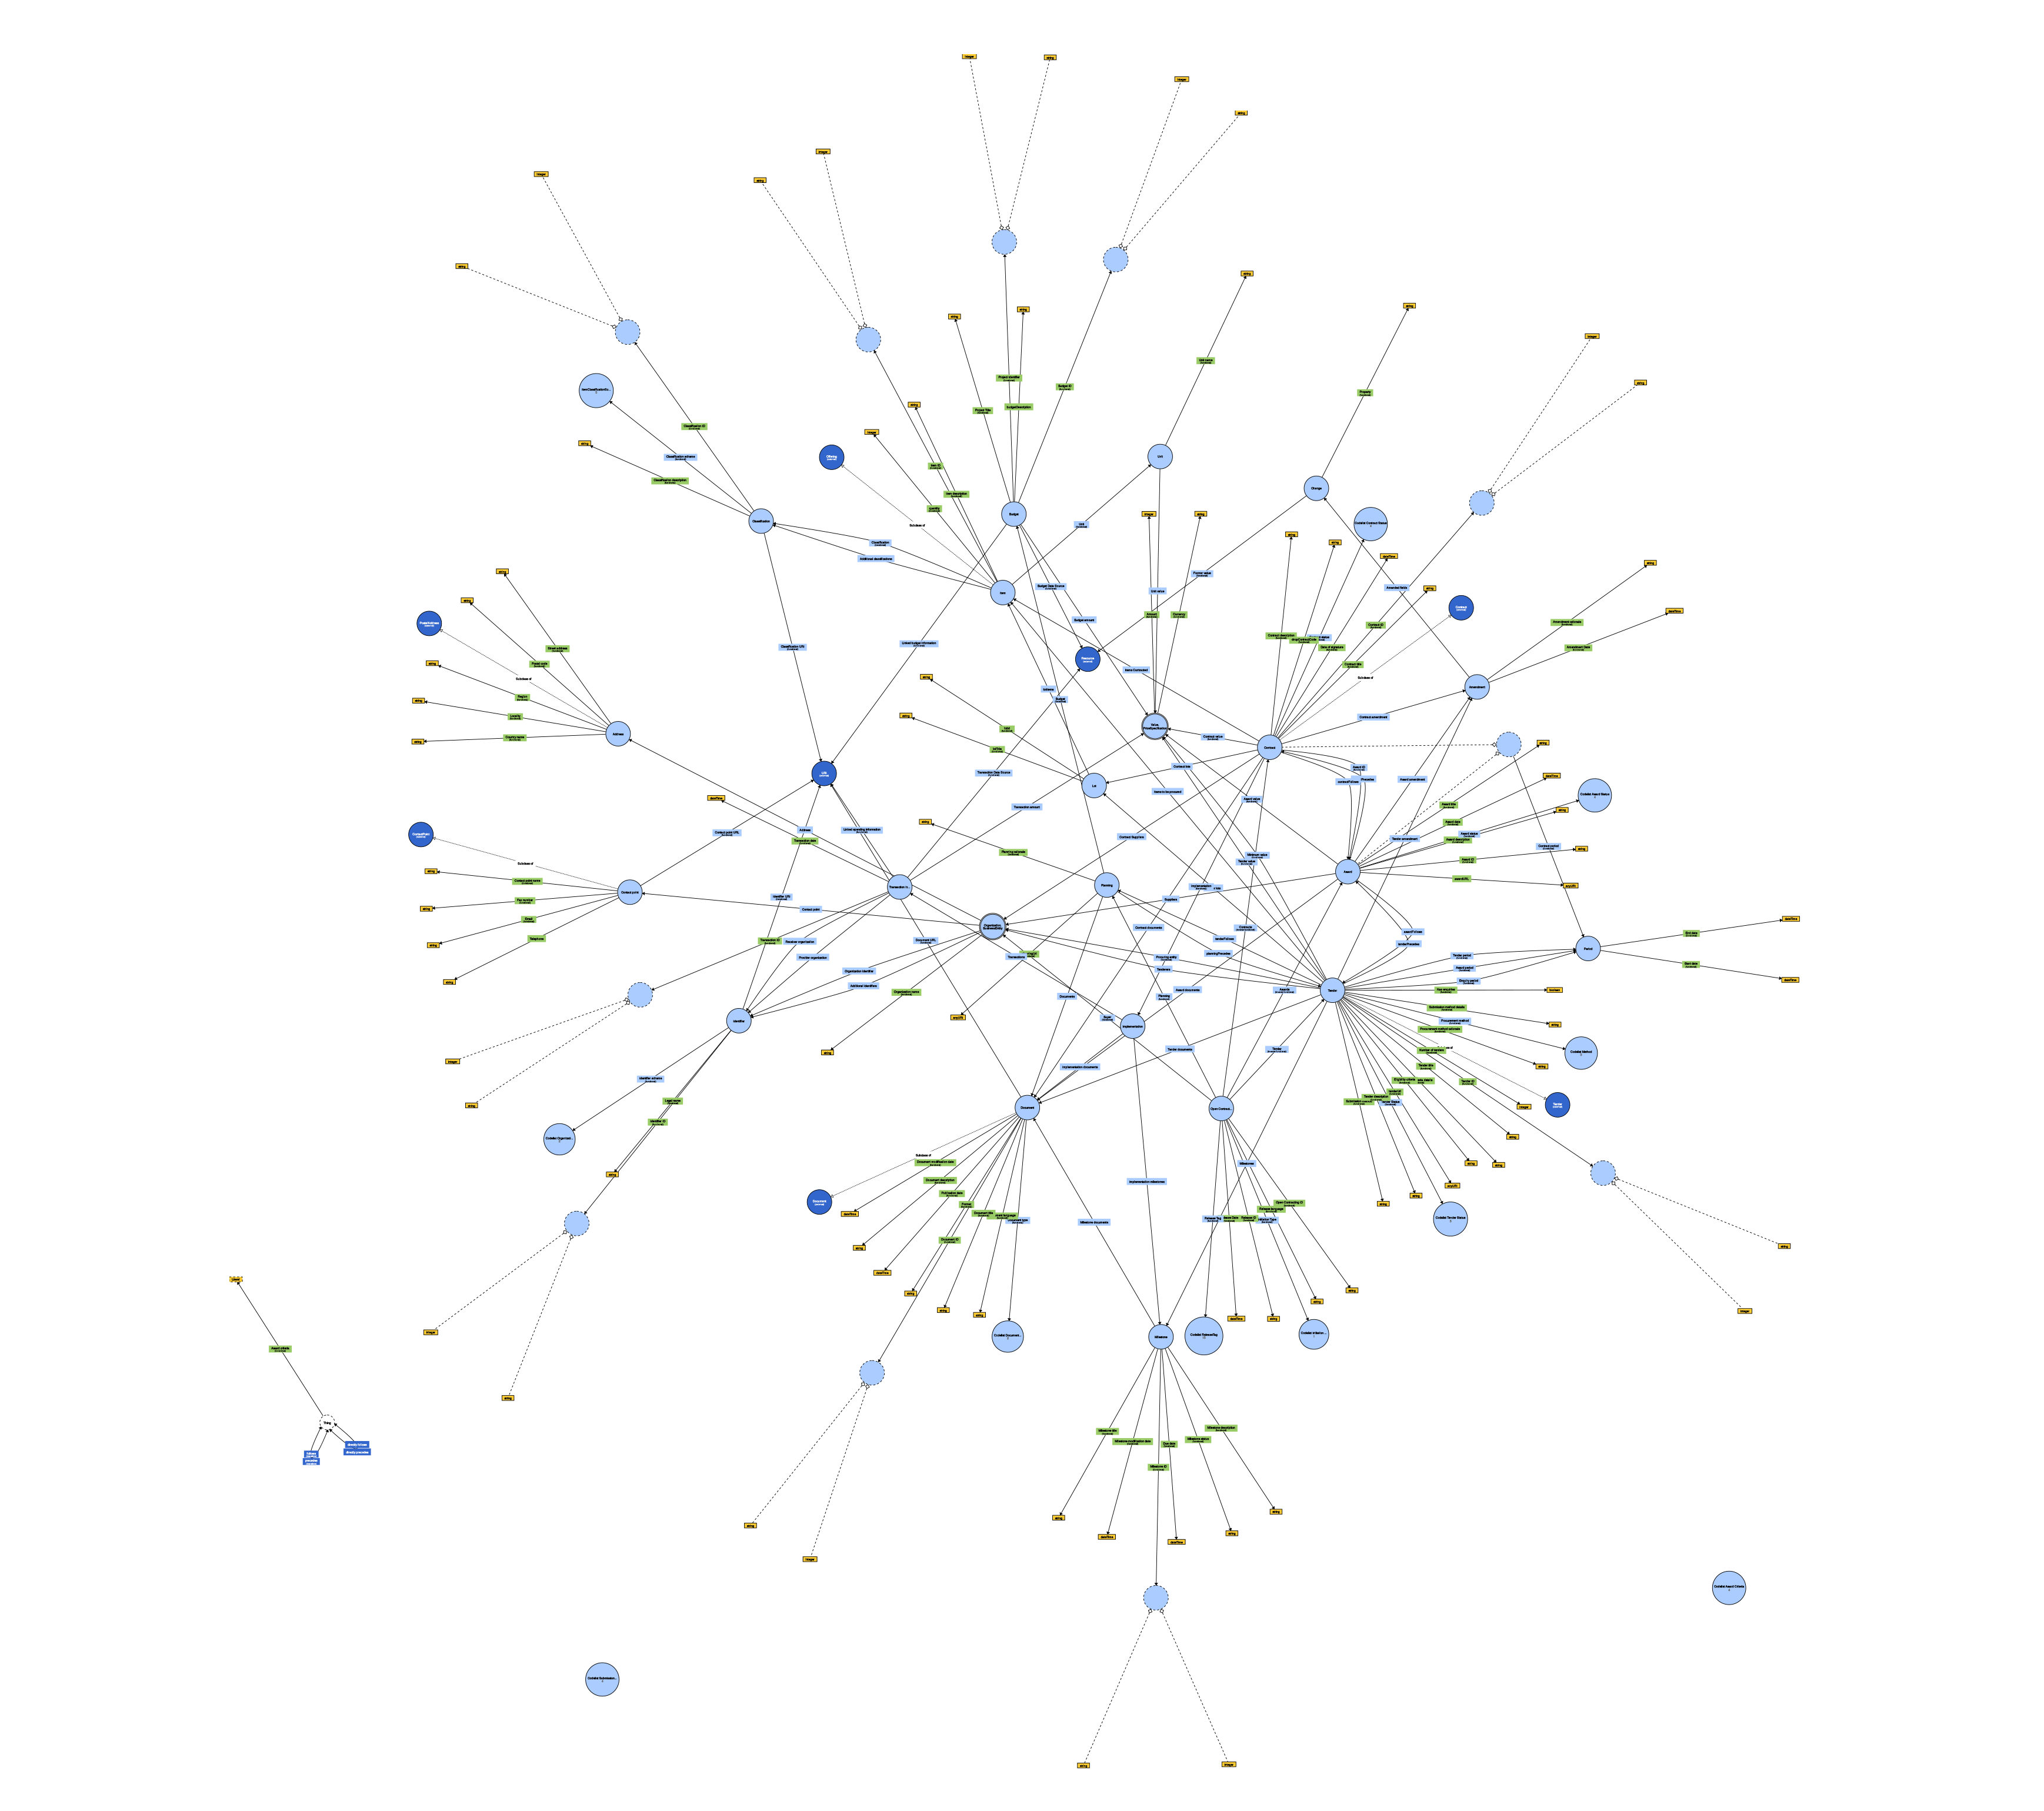
\includegraphics[width=180mm]{figuras/grafoOCDS.png}
    \caption{Grafo de la ontología desarrollada}
    \label{img:grafo ontologia desarrolla}
    \end{figure}

    \begin{figure}[ht!]
        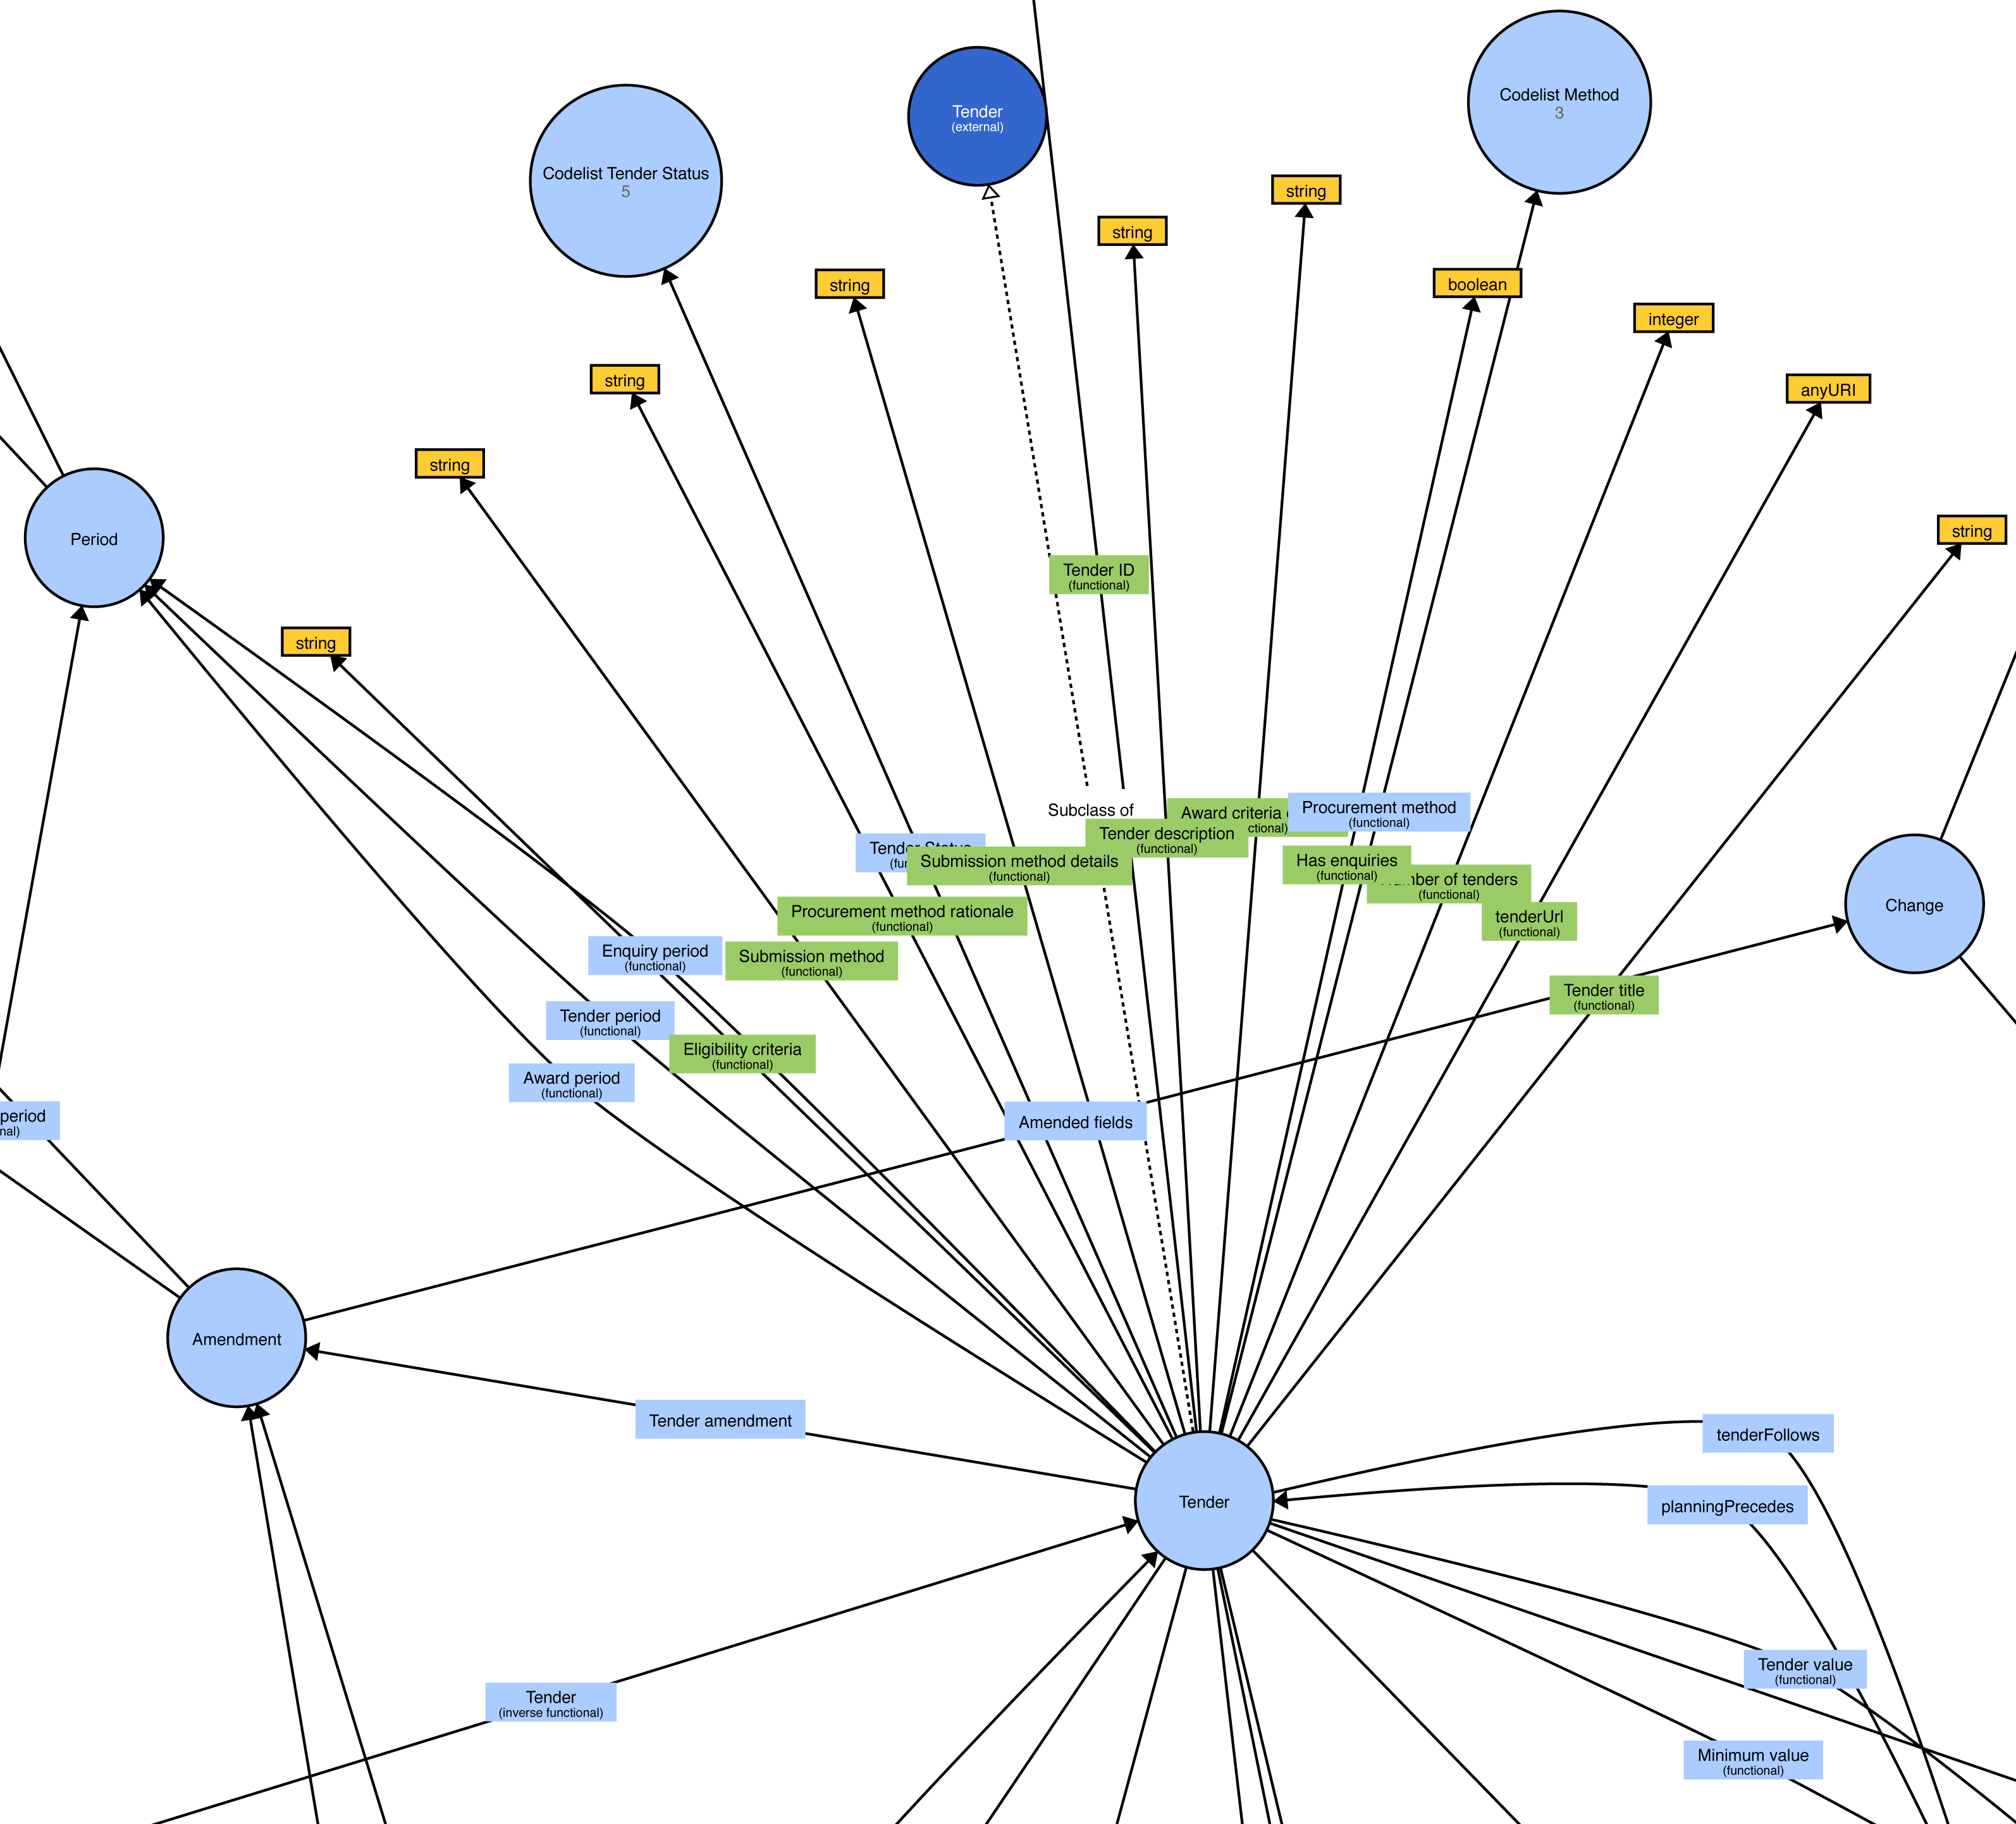
\includegraphics[width=150mm]{figuras/zoomTender.png}
        \caption{Acercamiento del Grafo de la ontología desarrollada en Convocatoria.}
        \label{img:zoomTender}
        \end{figure}


        \begin{figure}[ht!]
            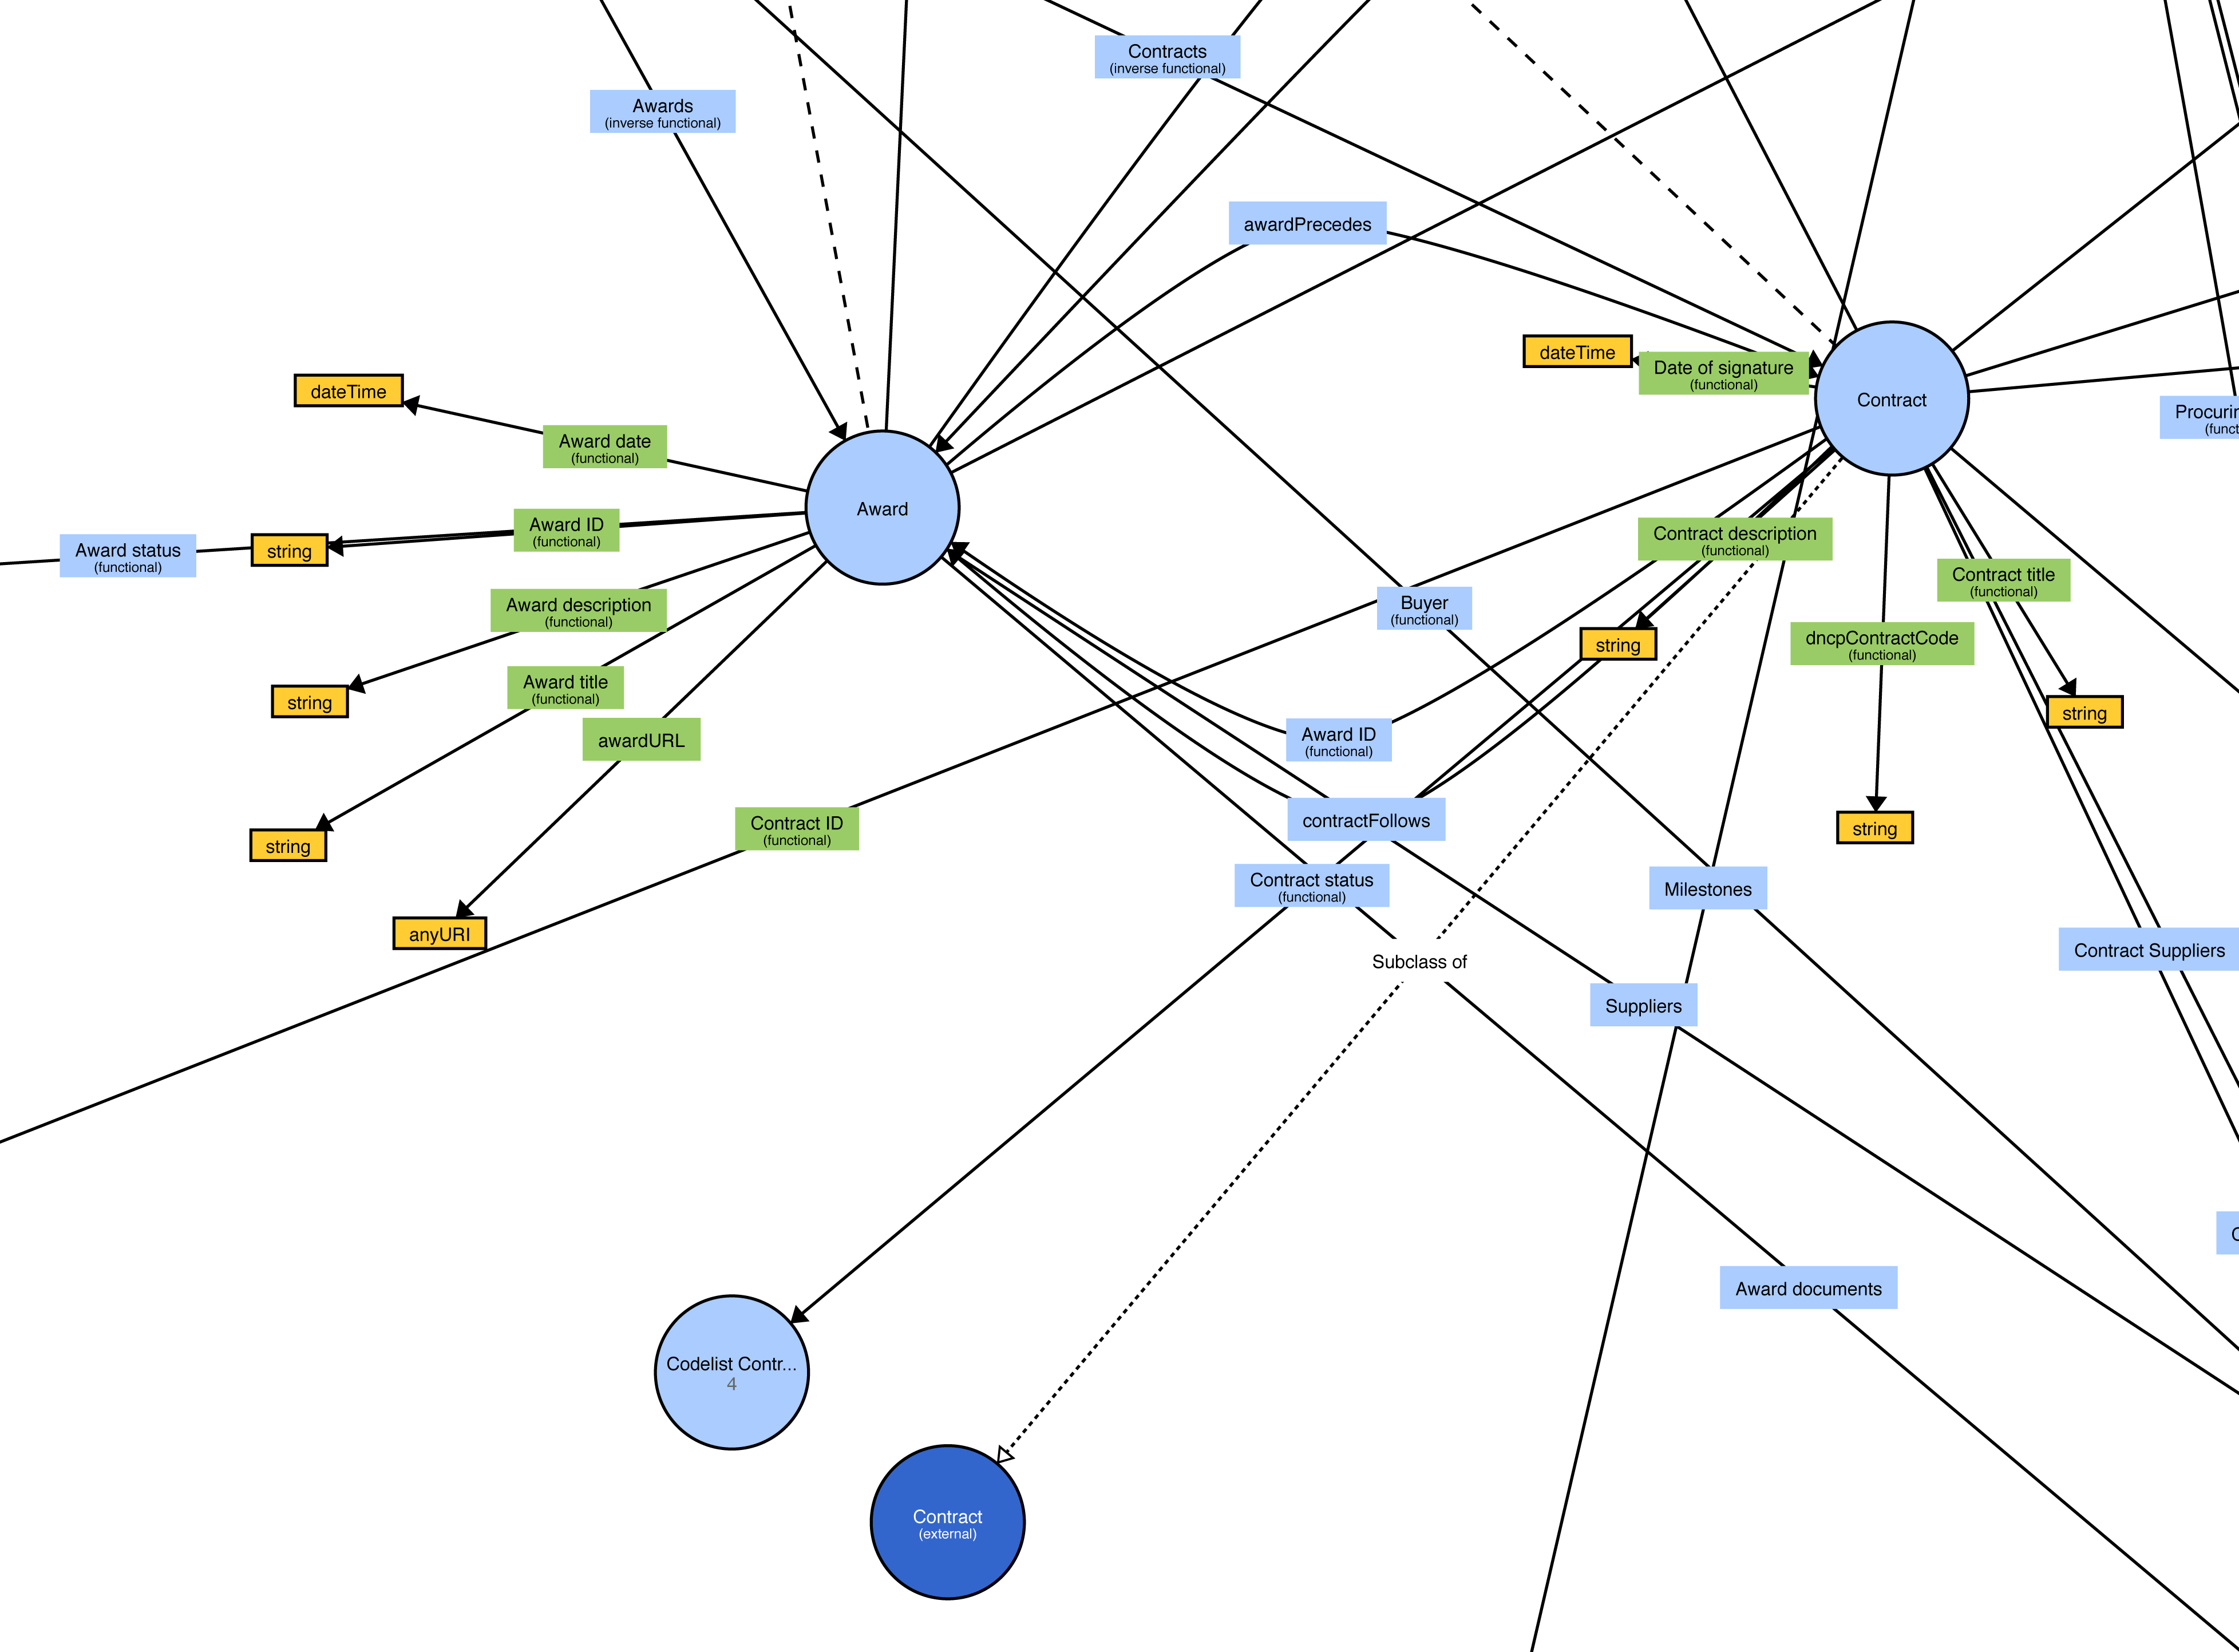
\includegraphics[width=150mm]{figuras/zoomContract.png}
            \caption{Acercamiento del Grafo de la ontología desarrollada en Contracto.}
            \label{img:zoomContract}
            \end{figure}



\section{Discusión del Capitulo}

En este capítulo se desarrolló una ontología teniendo como base de conocimiento un recurso no-ontológico (OCDS). Se utilizó la metodología NeOn y el software Protégé para el desarrollo de ontología. Las actividades principales fueron la planificación de actividades, especificación de los requerimientos, el reuso de recursos ontológicos y no-ontológicos. El resultado de todo este proceso fue una ontología desarrollada en lenguaje OWL que responde a la base de conocimiento de la OCDS y al esquema de datos de la DNCP teniendo en cuenta las buenas prácticas de desarrollo de ontologías propuestas por la metodología.





% \include{capitulo-ej/capitulo-ej}
% %!TEX root = ../main.tex
\chapter{Enfermedad de Chagas}
\label{chap:chagas}

La enfermedad de Chagas es considerada como negligenciada por la \gls{oms} y es causada por el protozoo flagelado Trypanosoma Cruzi. Esta enfermedad es poco estudiada pese a que afecta a millones de personas, tiene una tasa muy alta de incidencia en países en vías de desarrollo y su tratamiento es  costoso~\cite{trouiller2002drug}. 

La enfermedad se puede observar desde México hasta Sudamérica, aunque se pueden presentar casos en Estado Unidos y Canadá. Las zonas rurales son las más afectada produciendo mas de 10.000 muertes al año~\cite{lozano2013global}. En etapas iniciales síntomas que presenta la enfermedad son fiebre, linfadenopatía, aumento del tamaño del hígado y bazo, miocarditis o meningoencefalitis. En casos crónicos se presentan los síntomas: cardiomiopatía, dilatación patológica del esófago y colon~\cite{nery1968surto}. 

El método de transmisión es por medio de las heces de insectos triatominos hematófagos. Los cuales habitan principalmente en las grietas de viviendas precariamente construidas en zonas rurales. La transmisión también puede darse por medio de transfusiones de sangre, trasplante de órganos y de madres infectadas a los hijos durante el embarazo, pero estos casos son mas raros.

El parásito Trypanosoma cruzi, tiene un ciclo biológico complejo, su morfología y expresión antigénica cambia de acuerdo al lugar donde se encuentra. El parásito presenta tres tipos morfológicos funcionales: epimastigotes, tripomastigotes y amastigotes como se muestra en la Figura \ref{img:imagen-amastigotes1}. El tipo morfológico que estudiaremos es el amastigote en el cual el flagelo esta reducido o ausente.

\begin{figure}[h!]
\centering
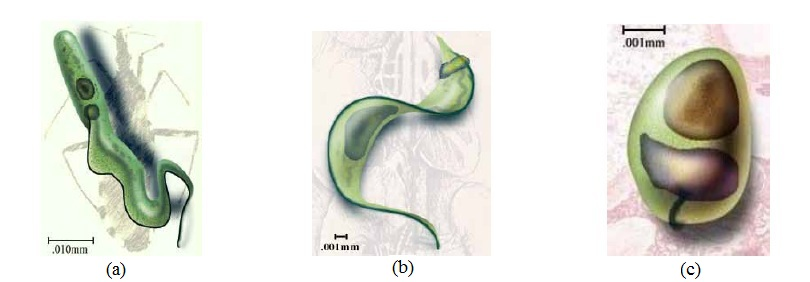
\includegraphics[width=90mm]{./figuras/amastigotes1.jpg}
\caption{(a) Epimastigotes. (b) Tripomastigotes. (c) Amastigotes}
\label{img:imagen-amastigotes1}
\end{figure}

El primer paso para determinar la eficacia de nuevos fármacos antichagasicos y así reducir el costo del tratamiento es el recuento de la forma parasitaria intracelular(amastigote) al microscopio~\cite{de2006analise}. 

En el contexto del tratamiento de las imágenes de amastigotes intracelulares de Trypanosoma Cruzi se citan trabajos que segmentan las imágenes a partir de la adquisición automatizada de imágenes de fluorescencia~\cite{engel2010image}~\cite{nohara2010high}. Las técnicas anteriores son específicas para el tipo de imágenes a la cual fueron aplicadas y es necesaria la adaptación de las mismas para cada tipo celular.

\begin{figure}[h!]
\centering
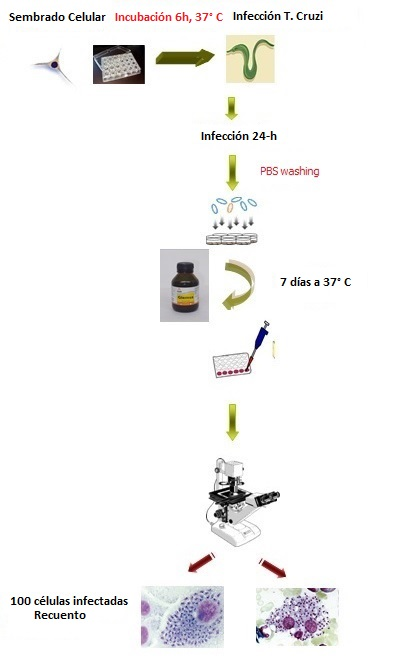
\includegraphics[width=90mm]{./figuras/amastigotes2.jpg}
\caption{Recuento de amastigotes vistos en el microscopio electrónico}
\label{img:imagen-amastigotes2}
\end{figure}

Como se muestra en la Figura \ref{img:imagen-amastigotes2} para realizar el conteo de forma manual de la cantidad de amastigotes presentes en las células infectadas las mismas son teñidas con el colorante Giemsa. Los núcleos y los amastigotes son teñidos de un color azul oscuro lo que permite que sean visualizadas y distinguidas al microscopio con un aumento de 1000x. Con el objetivo de disminuir los errores del investigador debido a la subjetividad de la técnica, el recuento se realiza por triplicado y se promedian los resultados~\cite{mendez1996leishmania}.

Para realizar el conteo de forma automática se puede utilizar la transformada de watershed con marcadores internos y externos como técnica de segmentación y la etiquetación de componentes conectados para el conteo. Este proceso ya se ha realizado en imágenes en escala de grises y demuestra ser eficiente y tener una baja tasa de error~\cite{noguera2013mathematical}. El trabajo presentado por Vázquez et al. solo se ha realizado en imágenes en escala de grises, esto deja abierta la posibilidad de mejorar la segmentación al obtener mayor información mediante el uso de imágenes a color.

\section{Resumen}

En este capítulo se presentaron los conceptos mas relevantes de la enfermedad de chagas, considerada como negligenciada por la \gls{oms}, el cual es producido por el parásito Trypanosoma cruzi. El parásito puede tener varias formas y la que estudiaremos se denomina amastigote. La segmentación de los componentes en imágenes celulares es importante para realizar el conteo de los amastigotes y así determinar la eficacia de los fármacos antichagasicos.
% %!TEX root = ../tesis.tex
\chapter{Imágenes a Color}
\label{chap:color}
En este capítulo se definen los conceptos básicos de imágenes digitales, así también los espacios de color utilizados en este trabajo. 

\section{Imágenes Digitales}
El píxel es la unidad básica de una imagen digital. Un píxel contiene información sobre el punto de color. Para poder visualizar, almacenar y procesar dicha información, se debe conocer el espacio de color en el cual está representado.

\addsymbol{symbol:F}
\addsymbol{symbol:e}
\addsymbol{symbol:d}
\addsymbol{symbol:n}
Una imagen digital consiste en un conjunto de píxeles. La definición formal esta dada como $F:e\rightarrow d$, donde $e$ es un subconjunto discreto de una grilla rectangular $\mathbb{N}^{2}$ para imágenes en dos dimensiones y $d$ es el rango de valores permitidos para el píxel.
Los píxeles de imágenes binarias se representan con un único valor en un rango de [0, 1]. Las imágenes en escala de grises utilizan un valor en el rango de [0, 255] como un subconjunto de $\mathbb{Z}$. Un píxel tiene asociado un color que se representa con un vector $(V_{1},V_{2},V_{3},...,V_{n})$ donde $n$ es el número de dimensiones del vector. 
\subsection{Espacios de Color}
Muchos espacios de color existen en el estado del arte. En esta sección se explican los espacios de color utilizados en este trabajo.
\subsubsection{RGB}
\addsymbol{symbol:r} \addsymbol{symbol:g} \addsymbol{symbol:b}
El espacio de color \gls{rgb} está especificado mediante cantidades positivas de los colores primarios, rojo ($r$), verde ($g$) y azul($b$), formando un cubo en el espacio 3D como se muestra en la Figura \ref{img:rgb-diagrama}. 
\begin{figure}[h!]
\centering
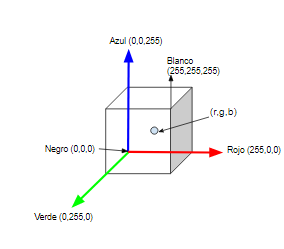
\includegraphics[width=80mm]{./figuras/diagrama-rgb.png}
\caption{Representación espacial del modelo de color RGB}
\label{img:rgb-diagrama}
\end{figure}
El espacio de color RGB es el que se emplea más comúnmente, es dependiente del dispositivo y se basa en la síntesis aditiva, en la cual un color puede ser representado mediante la mezcla por adición de los colores primarios~\cite{OrtizZamora2002}.
\begin{figure}[h!]
\centering
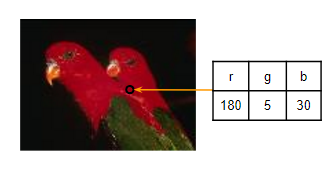
\includegraphics[width=80mm]{./figuras/ejemplo-rgb.png}
\caption{Ejemplo de un píxel representado en RGB}
\label{img:ejemplo-diagrama}
\end{figure}
El rango de valores que se maneja en RGB esta en el intervalo [0,255]. Las imágenes en el modelo de color RGB están formadas por 3 planos, uno por cada color primario. En la Figura \ref{img:ejemplo-diagrama} se muestra un ejemplo de la representación de un píxel en el espacio de color RGB. El color negro se encuentra en el origen de las coordenadas (0,0,0) y el color blanco en (255,255,255). El espacio de color RGB es útil para el procesamiento de imágenes cuando las mismas están expresadas en los 3 planos de colores~\cite{gonzalesdigital}. 

\subsubsection{HSI}
El espacio de color \gls{hsi} utiliza los valores de matiz, saturación e intensidad (en ingles hue, saturation e intensity) para representar los colores. Se puede representar como un doble cono o doble hexágono, en el cual los vértices corresponden con los colores negro y blanco. 
\begin{figure}[h!]
\centering
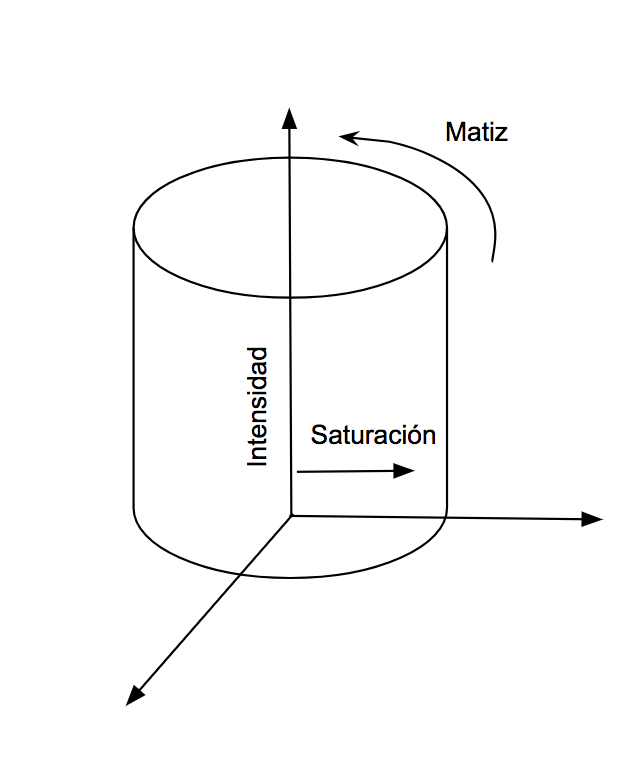
\includegraphics[width=70mm]{./figuras/diagrama-hsi.png}
\caption{Representación espacial del modelo de color HSI}
\label{img:hsi-diagrama}
\end{figure}

La representación cilíndrica de HSI se muestra en la Figura \ref{img:hsi-diagrama}, donde el ángulo en el sistema de coordenadas polar se corresponde con el matiz, la saturación se corresponde con la distancia radial y la intensidad esta dada por la distancia a lo largo del eje perpendicular al plano de coordenadas polares~\cite{OrtizZamora2002}.
\addsymbol{symbol:H}\addsymbol{symbol:S}\addsymbol{symbol:I}
Los valores de matiz ($H$), saturación ($S$) e intensidad ($I$) son calculados a partir de los valores RGB.

La transformación básica a partir de RGB de la matiz $H$ con rango [0,1] esta dada por:
\begin{equation}
H = \cos^{-1}\left[\frac{\frac{1}{2}\left[\left(r-g\right)+\left(r-b\right)\right]}{\sqrt{\left(r-g\right)^{2}+\left(r-b\right)\left(g-b\right)}}\right],
\end{equation}
donde si $b > g$, entonces $H=1-H$.

Posteriormente se calculan los valores de $S$ e $I$ como sigue:
\begin{equation}
S = 1-3\frac{min\left(r,g,b\right)}{r+g+b},
\end{equation}
\begin{equation}
I = \frac{r+g+b}{3}.
\end{equation}
\subsubsection{CIELab}
La \gls{cie} presentó el espacio de color $L^*a^*b^*$. Este espacio de color fue diseñado para que los colores que sean visualmente similares se representen en el espacio a unas distancias proporcionales a las diferencias visuales entre ellos, si la medida de distancia correcta es empleada~\cite{hanbury2001mathematical}. CIELab a diferencia del espacio RGB es independiente al dispositivo en el cual se representa.

\begin{itemize}
\addsymbol{symbol:l*}\addsymbol{symbol:a*}\addsymbol{symbol:b*}
\item $L^*$ representa la luminiscencia.
\item $a^*$ codifica la sensación rojo-verde, con $a^*$ positivo indicando un color rojo y $a^*$ negativo indicando un color verde.
\item $b^*$ codifica la sensación amarillo-azul, con $b^*$ positivo indicando un color amarillo y $b^*$ negativo indicando un color azul.
\end{itemize}
La representación espacial de CIELab se muestra en la Figura \ref{img:cielab-diagrama}. La escala de grises se encuentra en el eje $a^*=0$ y $b^*=0$ con negro en $L^*=0$ y blanco en $L^*=100$.

\begin{figure}[h!]
\centering
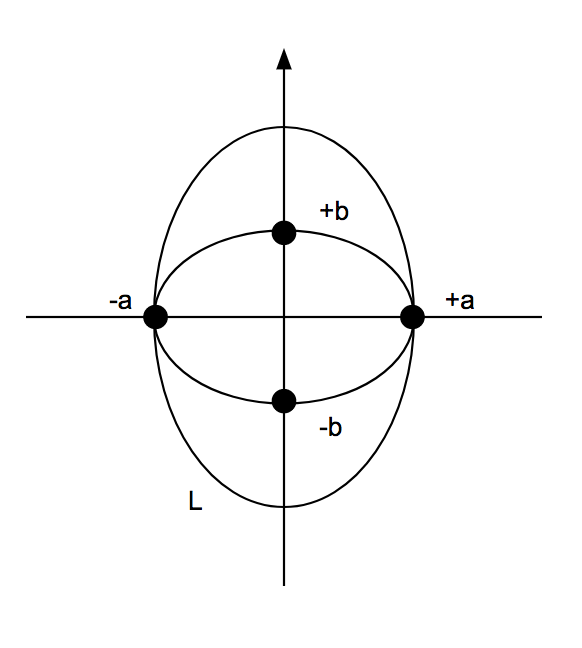
\includegraphics[width=80mm]{./figuras/diagrama-cielab.png}
\caption{Representación espacial del espacio de color CIELab}
\label{img:cielab-diagrama}
\end{figure}

La transformación del espacio de color RGB a \gls{cielab}~\cite{connolly1997study}, esta dada por la ecuación:
\addsymbol{symbol:x} \addsymbol{symbol:y} \addsymbol{symbol:z}
\addsymbol{symbol:r} \addsymbol{symbol:g} \addsymbol{symbol:b}
\begin{equation}
\begin{aligned}
X = 0,4303r + 0,3416g + 0,1784b, \\
Y = 0,2219r + 0,7068g + 0,0713b, \\
Z = 0,0202r + 0,1296g + 0,9393b. \\
\end{aligned}
\end{equation}
Se aplica la ecuación de CIELab
\begin{equation}
\label{formula:cielab}
\begin{aligned}
L^{*} = 116f\left(\frac{Y}{Y_{0}}\right) -16, \\
a^{*} = 500\left[f\left(\frac{X}{X_{0}}\right) - f\left(\frac{Y}{Y_{0}}\right)\right],\\
b^{*} = 200\left[f\left(\frac{Y}{Y_{0}}\right) - f\left(\frac{Z}{Z_{0}}\right)\right],
\end{aligned}
\end{equation}
donde
\addsymbol{symbol:f}\addsymbol{symbol:q}
\begin{equation}
\begin{aligned}
f(q) = \sqrt[3]{q} ~~ \text{si } q> 0,008856,\\
f(q) = 7,787q + \frac{16}{116}  ~~\text{si } q\leq 0,008856,
\end{aligned}
\end{equation}
para
\begin{equation}
\begin{aligned}
X_{0}=95.047, Y_{0}=100.00, Z_{0}=108.883,
\end{aligned}
\end{equation}
que son los valores del iluminante, en este caso el iluminante D65~\cite{connolly1997study}, 
el cual es un iluminante estándar de uso común definido por la CIE.
\addsymbol{symbol:elab}

La diferencia de color entre dos coordenadas en el espacio CIELab, $(L^{*}_{1},a^{*}_{1},b^{*}_{1})$ y $(L^{*}_{2},a^{*}_{2},b^{*}_{2})$ se define como $\Delta E_{Lab}$ y esta dada por la distancia Euclidiana~\cite{robertson1977cie}.
\begin{equation}
\label{formula:eucli}
\Delta E_{Lab} = \sqrt{(\Delta L^{*})^2 + (\Delta a^{*})^2 +(\Delta b^{*})^2},
\end{equation}
donde 
\addsymbol{symbol:deltal}
\addsymbol{symbol:deltaa}
\addsymbol{symbol:deltab}
\begin{equation}
\Delta L^{*} = L^{*}_{1} - L^{*}_{2},
\Delta a^{*} = a^{*}_{1} - a^{*}_{2},
\Delta b^{*} = b^{*}_{1} - b^{*}_{2}.
\end{equation}

\section{Resumen}

En este capítulo se presentaron los espacios de color más prevalentes en la literatura que serán utilizados para implementar la transformada de watershed y comparar el rendimiento de los mismos.

% %!TEX root = ../main.tex
\chapter{Transformada Watershed}
\label{chap:marco}
En este capítulo se definen los conceptos básicos de  ordenamiento vectorial y la matemática morfológica que serán utilizados posteriormente, así también la transformada de watershed por inundación y métodos de ordenes utilizados en este trabajo. 

\section{Matemática Morfológica}
La segmentación es el proceso de particionar imágenes digitales en múltiples segmentos. El objetivo de la segmentación es modificar y/o simplificar la forma en la que se representa una imagen, para que sea más significativa y fácil de analizar~\cite{wiki:segmentacion}. La matemática morfológica es una rama del análisis de imágenes basada en la teoría de conjuntos y principios algebraicos y geométricos~\cite{matheron2002birth}.

Los operadores básicos de la matemática morfológica son la erosión ($\varepsilon$) y la dilatación ($\delta$), que pueden ser definidos a partir del mínimo y el máximo respectivamente dentro de una ventana llamada elemento estructurante~\cite{noguera2014color}. 

Dada una ventana $E$, representada como el elemento estructurante, y una imagen $F$. 
\addsymbol{symbol:E} \addsymbol{symbol:F} 
\addsymbol{symbol:erosion} \addsymbol{symbol:dilatacion} \addsymbol{symbol:estructurante} 
La erosión ($\varepsilon$) de $F$ utilizando $E$ se puede definir como:
\begin{equation}
\varepsilon(F,E)(u,v)  = \min_{(i,j) \in E} \{F(u-i,v-j) + E(i,j) \},
\end{equation}
y la dilatación ($\delta$) de $F$ utilizando $E$ se puede definir como:
\begin{equation}
\delta(F,E)(u,v)  =  \max_{(i,j) \in E} \{F(u+i,v+j) - E(i,j) \}.
\end{equation}
\addsymbol{symbol:F}
\addsymbol{symbol:j}
La gradiente ($\gamma$) es el cambio direccional en la intensidad o color de una imagen. La gradiente ($\gamma$) es la resultante de la diferencia entre la dilatación ($\delta$) y la erosión ($\varepsilon$) de la imagen $F$~\cite{beucher}, se define como:
\begin{equation}
\gamma(F,E)(u,v) = \delta(F,E)(u,v) - \varepsilon(F,E)(u,v).
\end{equation}
\addsymbol{symbol:F}
\addsymbol{symbol:gradiente}
En escala de grises obtener la relación de orden entre los pixeles es trivial, debido a que están clasificados de acuerdo al orden natural de los valores que representan la intensidad de los píxeles. En imágenes a color los píxeles están representados por vectores. Un problema abierto es la extensión de la matemática morfológica para imágenes multivaloradas, como son las imágenes a color~\cite{aptoula2007}.
Los principales tipos de procesamiento morfológico para imágenes multivaloradas son~\cite{aptoula2007}:
\begin{itemize}
\item Procesamiento Marginal: en el procesamiento marginal cada canal es procesado de manera independiente y no existe la correlación entre los canales.
\item Procesamiento Vectorial: en el procesamiento vectorial se procesan todos los canales de manera conjunta. Se considera a los píxeles como vectores, y son tratados como una unidad de procesamiento. Requiere de un esquema de ordenamiento vectorial.
\end{itemize}

El procesamiento marginal tiene como principal desventaja la pérdida de información de la imagen al procesar por separado cada uno de los canales. Por otra parte, el procesamiento vectorial aprovecha dicha información obteniendo mejores resultados.
\section{Ordenamiento Vectorial}
La Matemática Morfológica requiere establecer una relación de orden entre los colores, representados por vectores, para ser extendida a color. 
En general, una relación binaria $\beta$ en un conjunto $D$ es:
\addsymbol{symbol:beta}\addsymbol{symbol:D}
\begin{enumerate}
\item Reflexivo si $\boldsymbol a \beta \boldsymbol a, \forall \boldsymbol a \in D$,
\item Anti-Simétrico si $\boldsymbol a \beta \boldsymbol b$ y  $\boldsymbol b \beta \boldsymbol a \Rightarrow \boldsymbol a = \boldsymbol b, \forall \boldsymbol a, \boldsymbol b \in  D$,
\item Transitivo $\boldsymbol a \beta \boldsymbol b$ y $\boldsymbol b \beta \boldsymbol c \Rightarrow \boldsymbol a \beta \boldsymbol c, \forall  \boldsymbol a, \boldsymbol b, \boldsymbol c \in D$,
\item Total si $\boldsymbol a \beta \boldsymbol b$ o $\boldsymbol b \beta \boldsymbol a, \forall \boldsymbol a, \boldsymbol b \in D$.
\end{enumerate}

La relación de orden $\leq$ (menor o igual) es requerida para la relación binaria $\beta$.
Cuando la relación de orden $\leq$ cumple con las restricciones 1 y 3 es llamada pre-orden. Una relación de orden es considerada como un ordenamiento si además de cumplir con las restricciones de una relación de pre-orden, también cumple con la restricción 2.
Adicionalmente a todo lo anterior, la relación $\leq$ debe cumplir la restricción 4 para ser considerado como orden total, sino es considerado como orden parcial.

Las técnicas de ordenamiento vectorial pueden ser clasificadas en los siguientes grupos~\cite{barnett1976ordering}:
\begin{itemize}
\item Ordenamiento Marginal (Ordenamiento M): Este ordenamiento cada componente compara el color de manera independiente.
\item Ordenamiento Condicional (Ordenamiento C): Un componente marginal es seleccionado secuencialmente para ordenar los vectores, dependiendo de las diferentes condiciones. Un ejemplo muy utilizado en el Ordenamiento C es el orden lexicográfico, que utiliza todos los componentes disponibles de los vectores a ser ordenados.
\item Ordenamiento Parcial (Ordenamiento P): Este ordenamiento esta basado en la división de los vectores en grupos de equivalencia, tal que entre los grupos existe un orden. Algunos ordenamientos totales son considerados dentro de esta clase.
\item Ordenamiento Reducido (Ordenamiento R): Los vectores son reducidos a valores escalares y posteriormente son clasificados mediante su orden escalar natural. Por ejemplo, un ordenamiento R en $\mathbb{Z}^{n}$ puede considerarse tras definir una transformación $T : \mathbb{Z}^{n} \rightarrow \mathbb{R}$ y posteriormente ordenar mediante orden escalar de su proyección en $\mathbb{Z}^{n}$ por $T$.
\begin{equation}
\forall q,q^{\prime}\in\mathbb{R}^{n} 
q \leq q^{\prime} \Leftrightarrow T\left(q\right) \leq T\left(q^{\prime}\right).
\end{equation}
\end{itemize}
\section{Ordenamientos}
\label{chap:marco}
A continuación se presentan los ordenamientos utilizados en este trabajo. Se utilizan píxeles $q$, $s$ y $t$ y sus respectivos componentes $(V_{1},V_{2},V_{3})$, $(V_{1},V_{2},V_{3})$ y $(V_{1},V_{2},V_{3})$ para ejemplificar el comportamiento de los ordenamientos que se explican posteriormente.

\subsection{Lexicográfico}
\label{chap:marco-lex}
El orden lexicográfico es también conocido como el orden de diccionario~\cite{chanussot1998total}~\cite{talbot98complete}. Una prioridad es asignada a cada componente del vector par que unos tengan mayor importancia que los otros al momento de realizar una comparación y definir un orden.
\addsymbol{symbol:q} \addsymbol{symbol:V}
\addsymbol{symbol:n} \addsymbol{symbol:lex}
\begin{equation}
q \leq q^{\prime} \Leftrightarrow \left[  V_{1},...,V_{n} \right]^{T} \leq_{L} \left[  V^{\prime}_{1},...,V^{\prime}_{n} \right]^{T},
\end{equation}
donde $\leq_{L}$ es el orden lexicográfico.

Para determinar si uno es mayor al otro se realiza los siguiente: se establece la prioridad entre los componentes, es decir, el componente $r$ tiene la mayor prioridad, luego el componente $g$ y por ultimo el $b$. Luego se compara inicialmente el primer componente con mayor prioridad, en caso de darse una igualdad, se compara el siguiente componente de mayor prioridad y así sucesivamente. De acuerdo a como se realice la selección de la prioridad, se podrían obtener resultados distintos.
\addsymbol{symbol:vec}
Por ejemplo, dados los píxeles $q=\left\{2,4,9\right\}, s=\left\{2,5,9\right\}, t=\left\{8,4,1\right\}$, se comparan los valores del componente con mayor prioridad, donde el componente $r$ tiene mayor prioridad, luego $g$ y $b$. Se puede observar que $t>s$ y $t>q$. No se puede determinar el orden entre $q$ y $s$, por lo cual se toma el siguiente componente con mayor prioridad, donde se puede observar que $t>s>q$.

\subsection{Alpha modulus lexicográfico}
\label{chap:marco-alphalex}
Una extensión del ordenamiento lexicográfico mostrado anteriormente fue propuesta en~\cite{angulo2003morphologie} que consiste en utilizar un valor $\alpha$ que el usuario defina, para modificar el grado de influencia que posee el primer componente. Se formula de la siguiente manera:
\addsymbol{symbol:q} \addsymbol{symbol:V}
\addsymbol{symbol:n} \addsymbol{symbol:lex}
\addsymbol{symbol:alpha}
\begin{equation}
q \leq q^{\prime} \Leftrightarrow \left[  \lceil V_{1}/\alpha\rceil , V_{2},...,V_{n} \right]^{T} \leq_{L} \left[  \lceil V^{\prime}_{1}/\alpha\rceil, V^{\prime}_{2},...,V^{\prime}_{n} \right]^{T}.
\end{equation}
\addsymbol{symbol:vec}
Por ejemplo, dados los píxeles $q=\left\{5,4,9\right\}, s=\left\{8,5,9\right\}, t=\left\{18,4,1\right\}$, se comparan los valores del componente con mayor prioridad dividido por el valor $\alpha$, donde se puede observar que $t>s$ y $t>q$, ya que $\lceil q_{1}/\alpha\rceil = 1,\lceil s_{1}/\alpha\rceil = 1,\lceil t_{1}/\alpha\rceil = 2$. No se puede determinar el orden entre $q$ y $s$, por lo cual se toma el siguiente componente con mayor prioridad, donde se puede observar que $t>s>q$.


\subsection{Vázquez et al}
\label{chap:marco-vazquez}
\addsymbol{symbol:T} \addsymbol{symbol:V} \addsymbol{symbol:w} \addsymbol{symbol:q}
\addsymbol{symbol:j} \addsymbol{symbol:F}
\addsymbol{symbol:n}\addsymbol{symbol:Sp}
\addsymbol{symbol:win}

Vázquez~\cite{noguera2014color} propuso una modificación del ordenamiento lexicográfico, tomando información de la imagen para obtener una transformación que se utiliza como el componente de mayor prioridad del orden lexicográfico.

La transformación propuesta por Vázquez en~\cite{noguera2014color} esta expresada como sigue: Para considerar la información local analizada por los operadores morfológicos, la imagen $F$ es particionada en ventanas denotadas por $win$, donde $win \subset F$. La transformada $T(q): \mathbb{Z}^{n}\rightarrow \mathbb{R}$ del píxel $q$ se obtiene mediante el producto escalar del vector $V = \left\{V_{1},V_{2},V_{3} \right\}$ correspondiente al píxel $q$ en el espacio de color $Sp$ con el vector de pesos $w = \left\{w1,w2,w3 \right\}$, es decir:
\begin{equation}
T\left(q\right) = \sum_{j=1}^n w_{j} \times V_{j}.
\end{equation}
\addsymbol{symbol:vec}
Por ejemplo, dados los píxeles $q=\left\{2,4,9\right\}, s=\left\{1,5,9\right\}, t=\left\{8,4,1\right\}$, utilizando la media en cada uno de los componentes, se forma el vector de pesos con los valores $w=\left\{5,6,9\right\}$, posteriormente se tienen los resultados:
$T(q)=2\times5+4\times6+9\times9=115,
T(s)=1\times5+5\times6+9\times9=116,
T(t)=8\times5+4\times6+1\times9=73$, donde se puede observar que $s>q>t$.

Las variaciones están dadas en el cálculo del vector de pesos $w$, para el cual se realizaron cálculos con la media, mínimo, máximo, entropia, moda, moda máximo, moda mínimo, suavidad y varianza de la imagen. Las comparaciones fueron realizadas en el espacio de color RGB para todas las variantes y se utiliza solo la transformada para la comparación debido a que para la transformada de watershed el hecho de que dos colores diferentes tengan la misma transformada no es un problema ya que se agruparán en el mismo nivel.

\subsection{Distancia euclidiana}
\label{chap:marco-distanciaeuclidianta}
Para el espacio de color RGB se realiza el cálculo con la distancia al origen, mientras que en el espacio de color CIELab se calcula con las distancias al origen, media y mediana de la imagen. 

Para el espacio de color CIELab se utiliza la fórmula descrita en \ref{formula:eucli}. Para el espacio de color RGB se utiliza la diferencia de color entre dos coordenadas $(r_{1},g_{1},b_{1})$ y $(r_{2},g_{2},b_{2})$ definido como $\Delta E_{rgb}$:~\cite{robertson1977cie}.
\addsymbol{symbol:r}\addsymbol{symbol:g}
\addsymbol{symbol:b}\addsymbol{symbol:ergb}
\begin{equation}
\label{formula:euclirgb}
\Delta E_{rgb} = \sqrt{(\Delta r)^2 + (\Delta g)^2 +(\Delta b)^2},
\end{equation}
donde 
\addsymbol{symbol:deltargbR}
\addsymbol{symbol:deltargbG}
\addsymbol{symbol:deltargbB}
\begin{equation}
\Delta r = r_{1} - r_{2},
\Delta g = g_{1} - g_{2},
\Delta b = b_{1} - b_{2}.
\end{equation}
\addsymbol{symbol:vec}
Por ejemplo, dados los píxeles $q=\left\{2,4,9\right\}, s=\left\{1,5,9\right\}, t=\left\{8,4,1\right\}$, utilizando la distancia al origen, se tienen los resultados:
$T(q)=\sqrt{(2-0)^{2}+(4-0)^{2}+(9-0)^{2}}=10.04$ ,
$T(s)=\sqrt{(1-0)^{2}+(5-0)^{2}+(9-0)^{2}}=10.34$ ,
$T(t)=\sqrt{(8-0)^{2}+(4-0)^{2}+(1-0)^{2}}=9$ , donde se puede observar que $s>q>t$.


\subsection{Entrelazado de bits}
\label{chap:marco-entrelazado}
El ordenamiento por entrelazado de bits consiste en una transformación inyectiva explotando la representación binaria de cada uno de los componentes, obteniendo un orden total en el espacio vectorial~\cite{chanussot1997bit}~\cite{chanussot1998total}.
Para un píxel $q$ con componentes ${x,y,z}$ en el espacio de color $Sp$, codificado en $k$ bits, la transformación por reducción $T: \mathbb{Z}^{n}\rightarrow \mathbb{Z}$ se calcula mediante la fórmula:
\addsymbol{symbol:q} \addsymbol{symbol:V}
\addsymbol{symbol:n} \addsymbol{symbol:k} 
\addsymbol{symbol:m} \addsymbol{symbol:T}
\addsymbol{symbol:j} \addsymbol{symbol:Sp}
\begin{equation}
T\left(q\right):\sum_{m=1}^k\left\{
2^{n.(k-m)}.\sum_{j=1}^n 2^{n-j}.V_{j,m}\right\},
\end{equation}
donde $V_{j,m}$ corresponde al m-ésimo bit del j-ésimo componente del píxel $q$. La representación binaria de $T(q)$ resultante se convierte en:
\begin{equation}
V_{1,1}V_{2,1}...V_{n,1}V_{1,2}V_{2,2}...V_{n,2}...V_{1,k}V_{2,k}...V_{n,k}.
\end{equation}
\addsymbol{symbol:vec}
Por ejemplo, dados los píxeles $q=\left\{2,4,9\right\}, s=\left\{1,5,9\right\}, t=\left\{8,4,1\right\}$, y la función de transformación T, los componentes expresados en 4 bits, se tienen los resultados:

$T(q)=\overbrace{0010}^2\overbrace{0100}^4\overbrace{1001}^9,
T(s)=\overbrace{0001}^1\overbrace{0101}^5\overbrace{1001}^9,
T(t)=\overbrace{1000}^8\overbrace{0100}^4\overbrace{0001}^1$, donde se puede observar que $t>q>s$.

\subsection{Ordenamiento utilizado por Meyer}
\label{chap:marco-meyer}
El ordenamiento de los píxeles utilizado en la propuesta de Meyer~\cite{Meyer} utiliza el espacio de color RGB. El mismo realiza una transformación por reducción a un valor escalar mediante la fórmula:
\addsymbol{symbol:r} \addsymbol{symbol:g}
\addsymbol{symbol:b} 
\begin{equation}
Max\left(|r_{s}-r_{t}|,|g_{s}-g_{t}|,|b_{s}-b_{t}|\right).
\end{equation}
Posteriormente el orden natural de los números es utilizado para realizar la comparación. Para la implementación se asume como píxel de referencia el origen $\left\{0,0,0\right\}$.
Por ejemplo, dados los píxeles $s=\left\{2,4,8\right\}, t=\left\{1,5,9\right\}$, se tienen los resultados:
$T(s)=Max\left(|2-0|,|4-0|,|8-0|\right)=8,
T(t)=Max\left(|1-0|,|5-0|,|9-0|\right)=9$, donde se puede observar que $t>s$. Podría darse el caso que para ambos píxeles se obtenga el mismo resultado, lo que haría que dos pixeles tengan la misma transformación y no se pueda determinar el orden entre $t$ y $s$.
\section{Algoritmo de watershed}
\label{chap:marco}

El algoritmo propuesto en este trabajo se basa en la implementación del algoritmo de Vincent y Soille~\cite{VincentSoille}, el cual propone un enfoque de crecimiento de regiones a partir de los mínimos locales. A continuación se muestra un ejemplo gráfico para mejorar el entendimiento. Se hace una analogía con la geografía como se muestra en la Figura \ref{img:relieve}(a). Cada uno de los relieves topográficos de la imagen son inundados con agua, donde las líneas watershed son las divisorias de distintos depósitos de agua~\cite{parwashed}. Las entradas del algoritmo son la gradiente morfológica de la imagen y los marcadores. La transformación watershed puede ser clasificada bajo el enfoque de segmentación basado en regiones. 

El algoritmo de watershed en escala de grises descrito por Vincent y Soille~\cite{VincentSoille} realiza una inundación por niveles, desde el mínimo hasta el máximo nivel de intensidad de los píxeles de la imagen. En las Figuras \ref{img:relieve}(b),(c) y (d) se muestra como se van inundando los niveles. Las zonas de baja intensidad se conocen como vasijas (basins en Inglés), por donde fluirá el agua e inundará toda la imagen; es decir, el agua fluirá en cada una de las vasijas identificadas a partir de los mínimos de la imagen. El proceso de inundación continúa hasta que las aguas de cuencas o vasijas contiguas se unan, formando líneas de unión que representarán las fronteras de regiones homogéneas, y constituyen el resultado de la segmentación~\cite{parwashed}, como se muestra en la Figura \ref{img:relieve}(e). El crecimiento de regiones se inicia a partir de marcadores obtenidos por la selección de todos los mínimos del gradiente, lo que podría producir una segmentación no deseada. En la Figura \ref{img:relieve}(e) se muestra como el objeto segmentado fue dividido en el medio, produciendo un resultado no deseado.
\begin{figure}[H]
\centering
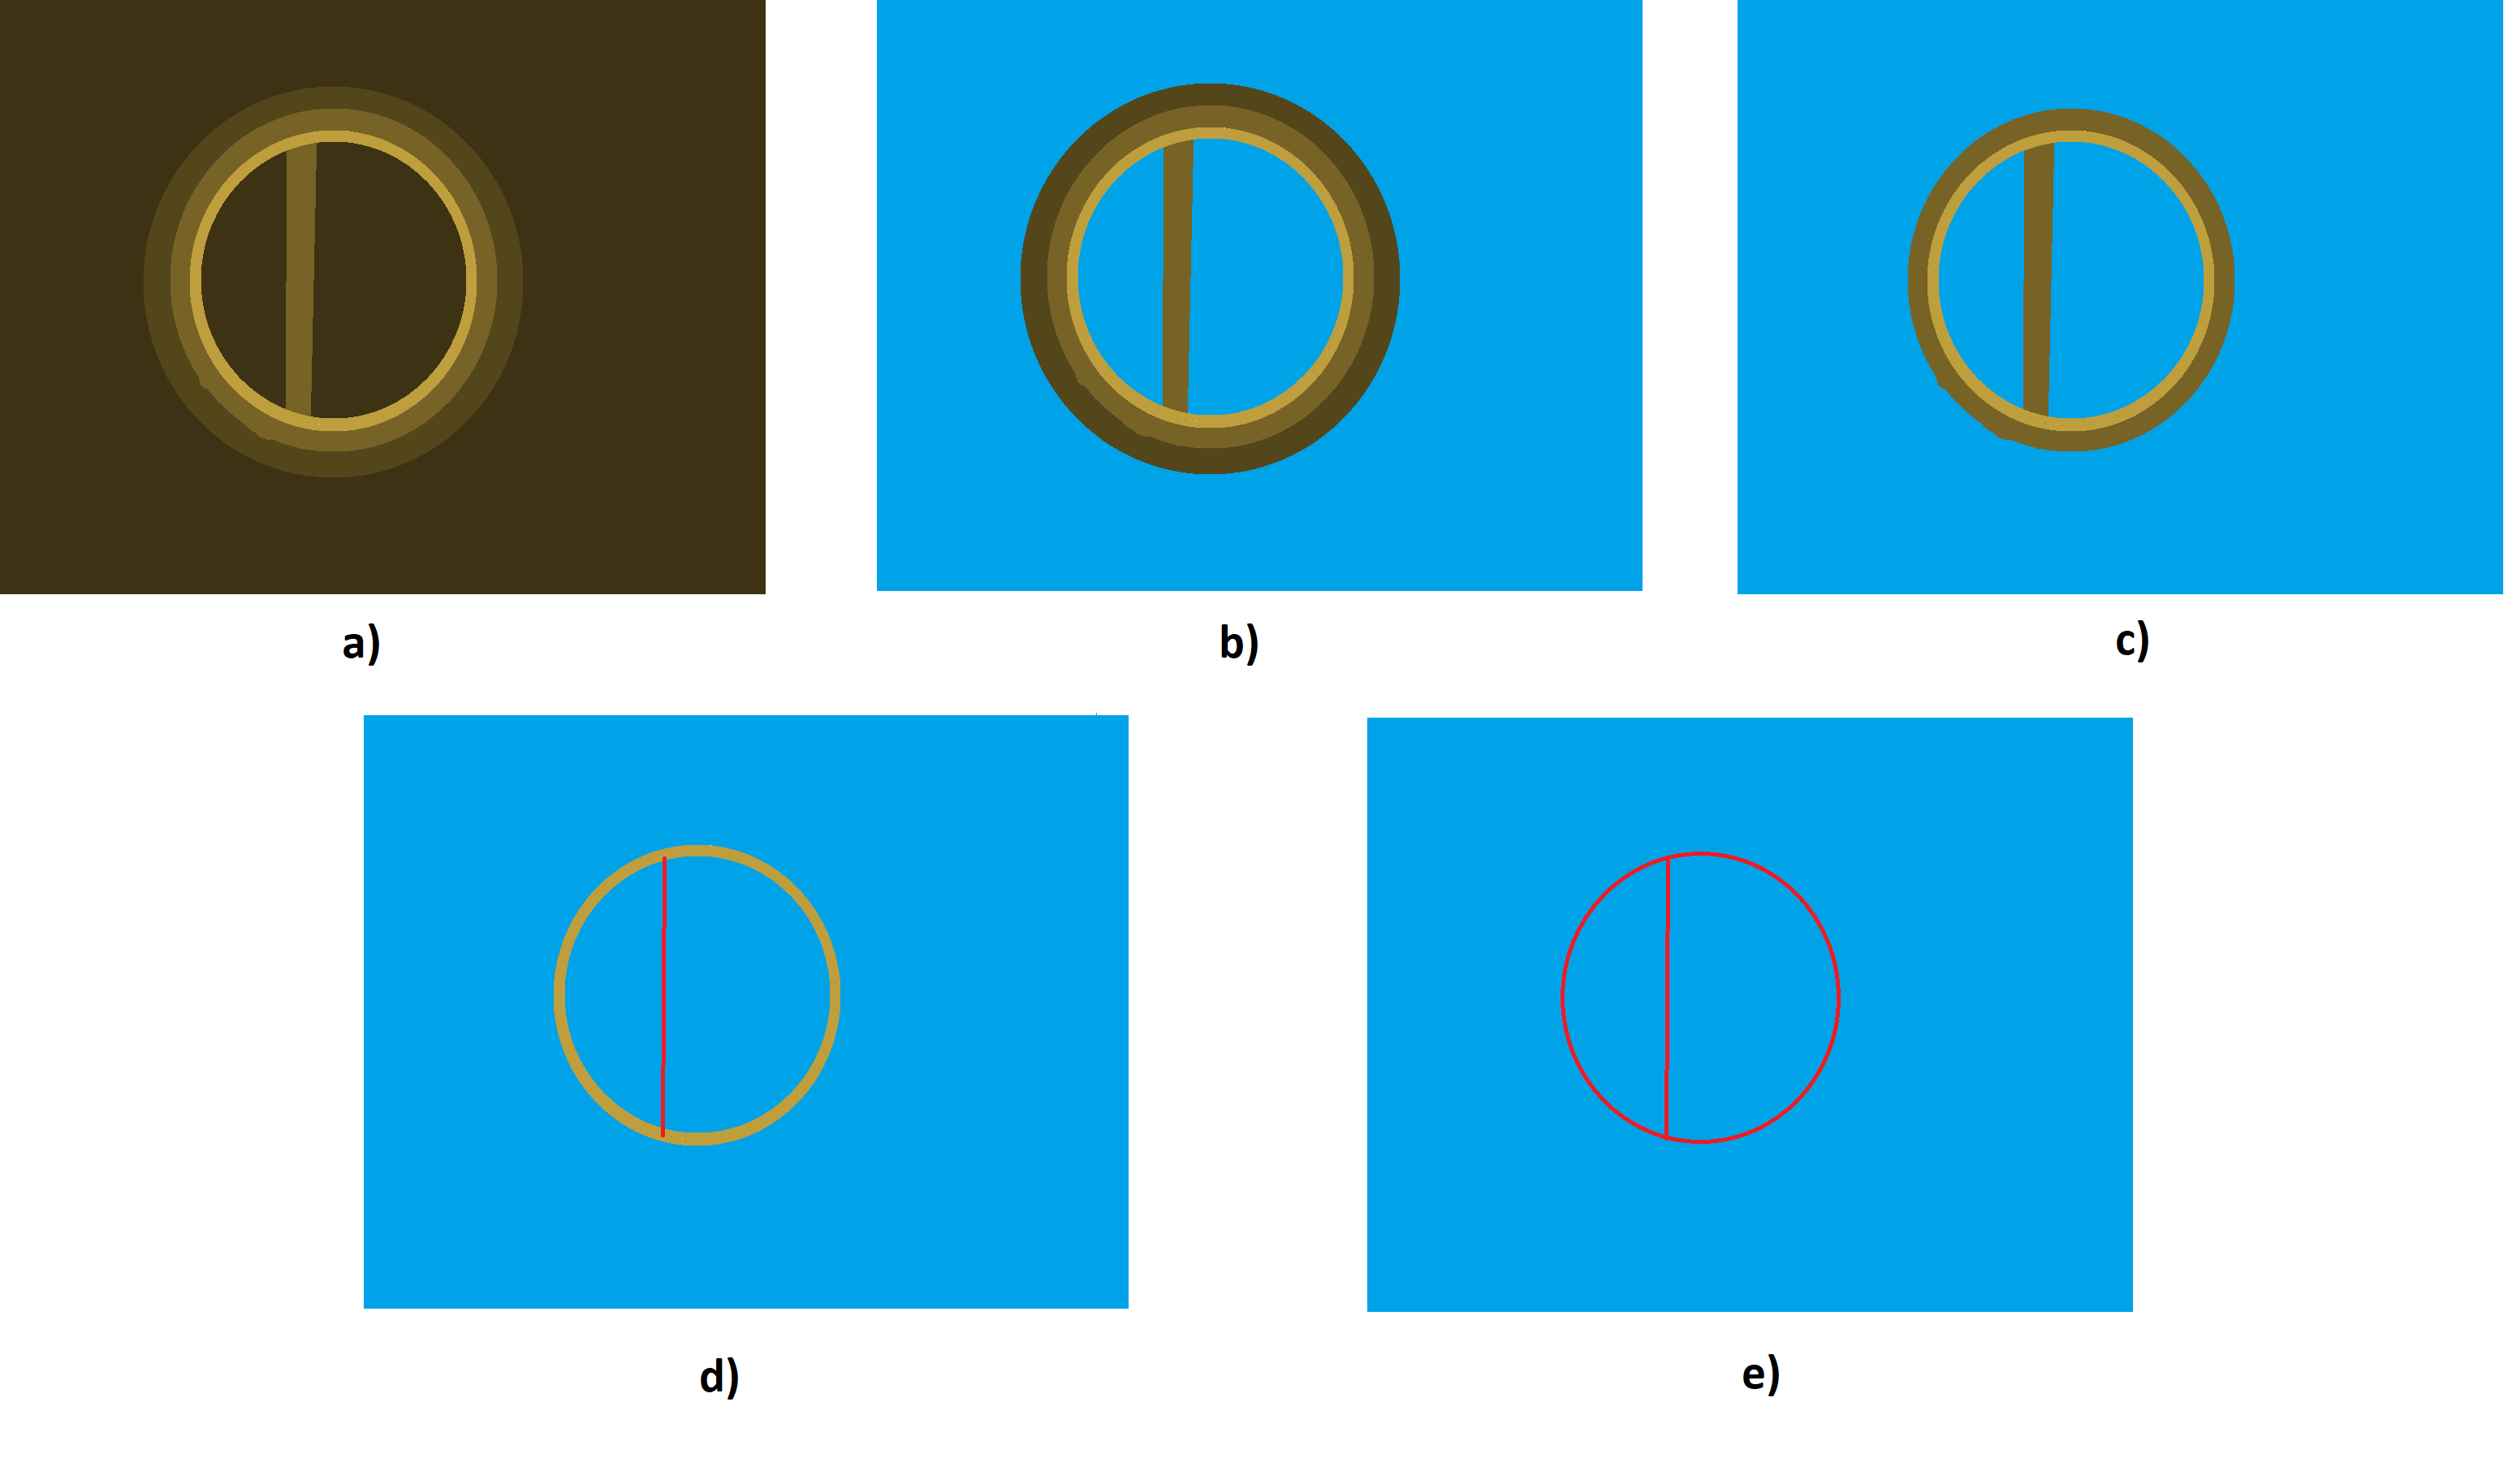
\includegraphics[width=150mm]{./imagenes/sin_marcadores.png}
\caption{Proceso de inundación con resultados no deseados}
\label{img:relieve}
\end{figure}

Al momento de la inundación, se tiene en cuenta una relación de orden dual entre los píxeles a ser inundados. La relación dual se entiende como la dependencia que existe entre dos criterios de ordenamiento, el orden de llegada a la cola y la altura de los píxeles. Un píxel de menor altura se debe inundar primero, así también los vecinos que se encuentren en una misma altura deben ser inundados antes de seguir con el orden anterior. Un algoritmo que simule la inundación tiene que poder reproducir la relación de orden dual, que naturalmente se obtiene con el uso de una cola de prioridad. Una cola de prioridad permite almacenar puntos en cualquier orden y devolverlos en el orden de la inundación.

El proceso de watershed para imágenes cromáticas puede afrontarse desde diversos enfoques. El empleo de información cromática en el proceso de watershed es posible por ejemplo, calculando el watershed en cada una de las señales cromáticas y combinar después los resultados~\cite{Saarinen}. Otra posibilidad es calcular el watershed directamente sobre la imagen a color~\cite{Meyer}.

La transformación watershed permite calcular los contornos más relevantes de la imagen, pudiendo así seleccionar los resultados deseados~\cite{Meyer}. En algunos casos donde las imágenes en escala de grises no presentan grandes variaciones de intensidad entre diferentes cuerpos, podría obtenerse una segmentación no esperada. Considere la misma imagen pero esta vez a color, podría tener los mismos niveles de intensidad pero en diferentes canales, en cuyo caso visualmente se distingue de manera fácil la diferencia entre diferentes cuerpos. El color es una propiedad distinguible entre diferentes regiones de una imagen por lo cual una segmentación a color puede tener mejores resultados que una en escala de grises~\cite{Lezoray}.

\subsection{Marcadores}
Generalmente los puntos iniciales de la inundación son mínimos locales y los marcadores denotan la cantidad de regiones a ser obtenidas luego del proceso de segmentación. En algunas imágenes se tiene la presencia de un gran número de mínimos locales, produciéndose sobre-segmentación en pequeñas regiones. Muchas de las regiones generadas no son importantes dentro de la imagen, o no representan objetos existentes en la imagen original.

La sobre-segmentación se puede disminuir utilizando métodos de mejora como filtros morfológicos. Además de ellos se podrían aplicar otras formas para evitar la sobre-segmentación, como es la selección de marcadores. Seleccionar marcadores en la imagen resuelve dicho problema iniciando el proceso de inundación desde los píxeles marcados, que representan los objetos deseados a segmentar en la imagen~\cite{Yang}. En este trabajo los marcadores fueron seleccionados manualmente.

La imagen que se muestra en la Figura \ref{img:relieve1}(a) contiene un objeto circular que se desea segmentar. Para evitar una segmentación no deseada fueron seleccionados dos marcadores, uno dentro del objeto deseado y otro en el fondo de la imagen, como se muestra en la Figura \ref{img:relieve1}(b). Posteriormente se inicia el proceso de inundación a partir de los marcadores como se muestra en las Figuras \ref{img:relieve1}(c), (d) y (e). En la Figura \ref{img:relieve1}(f) se muestra el resultado de la segmentación del objeto deseado.


\begin{figure}[H]
\centering
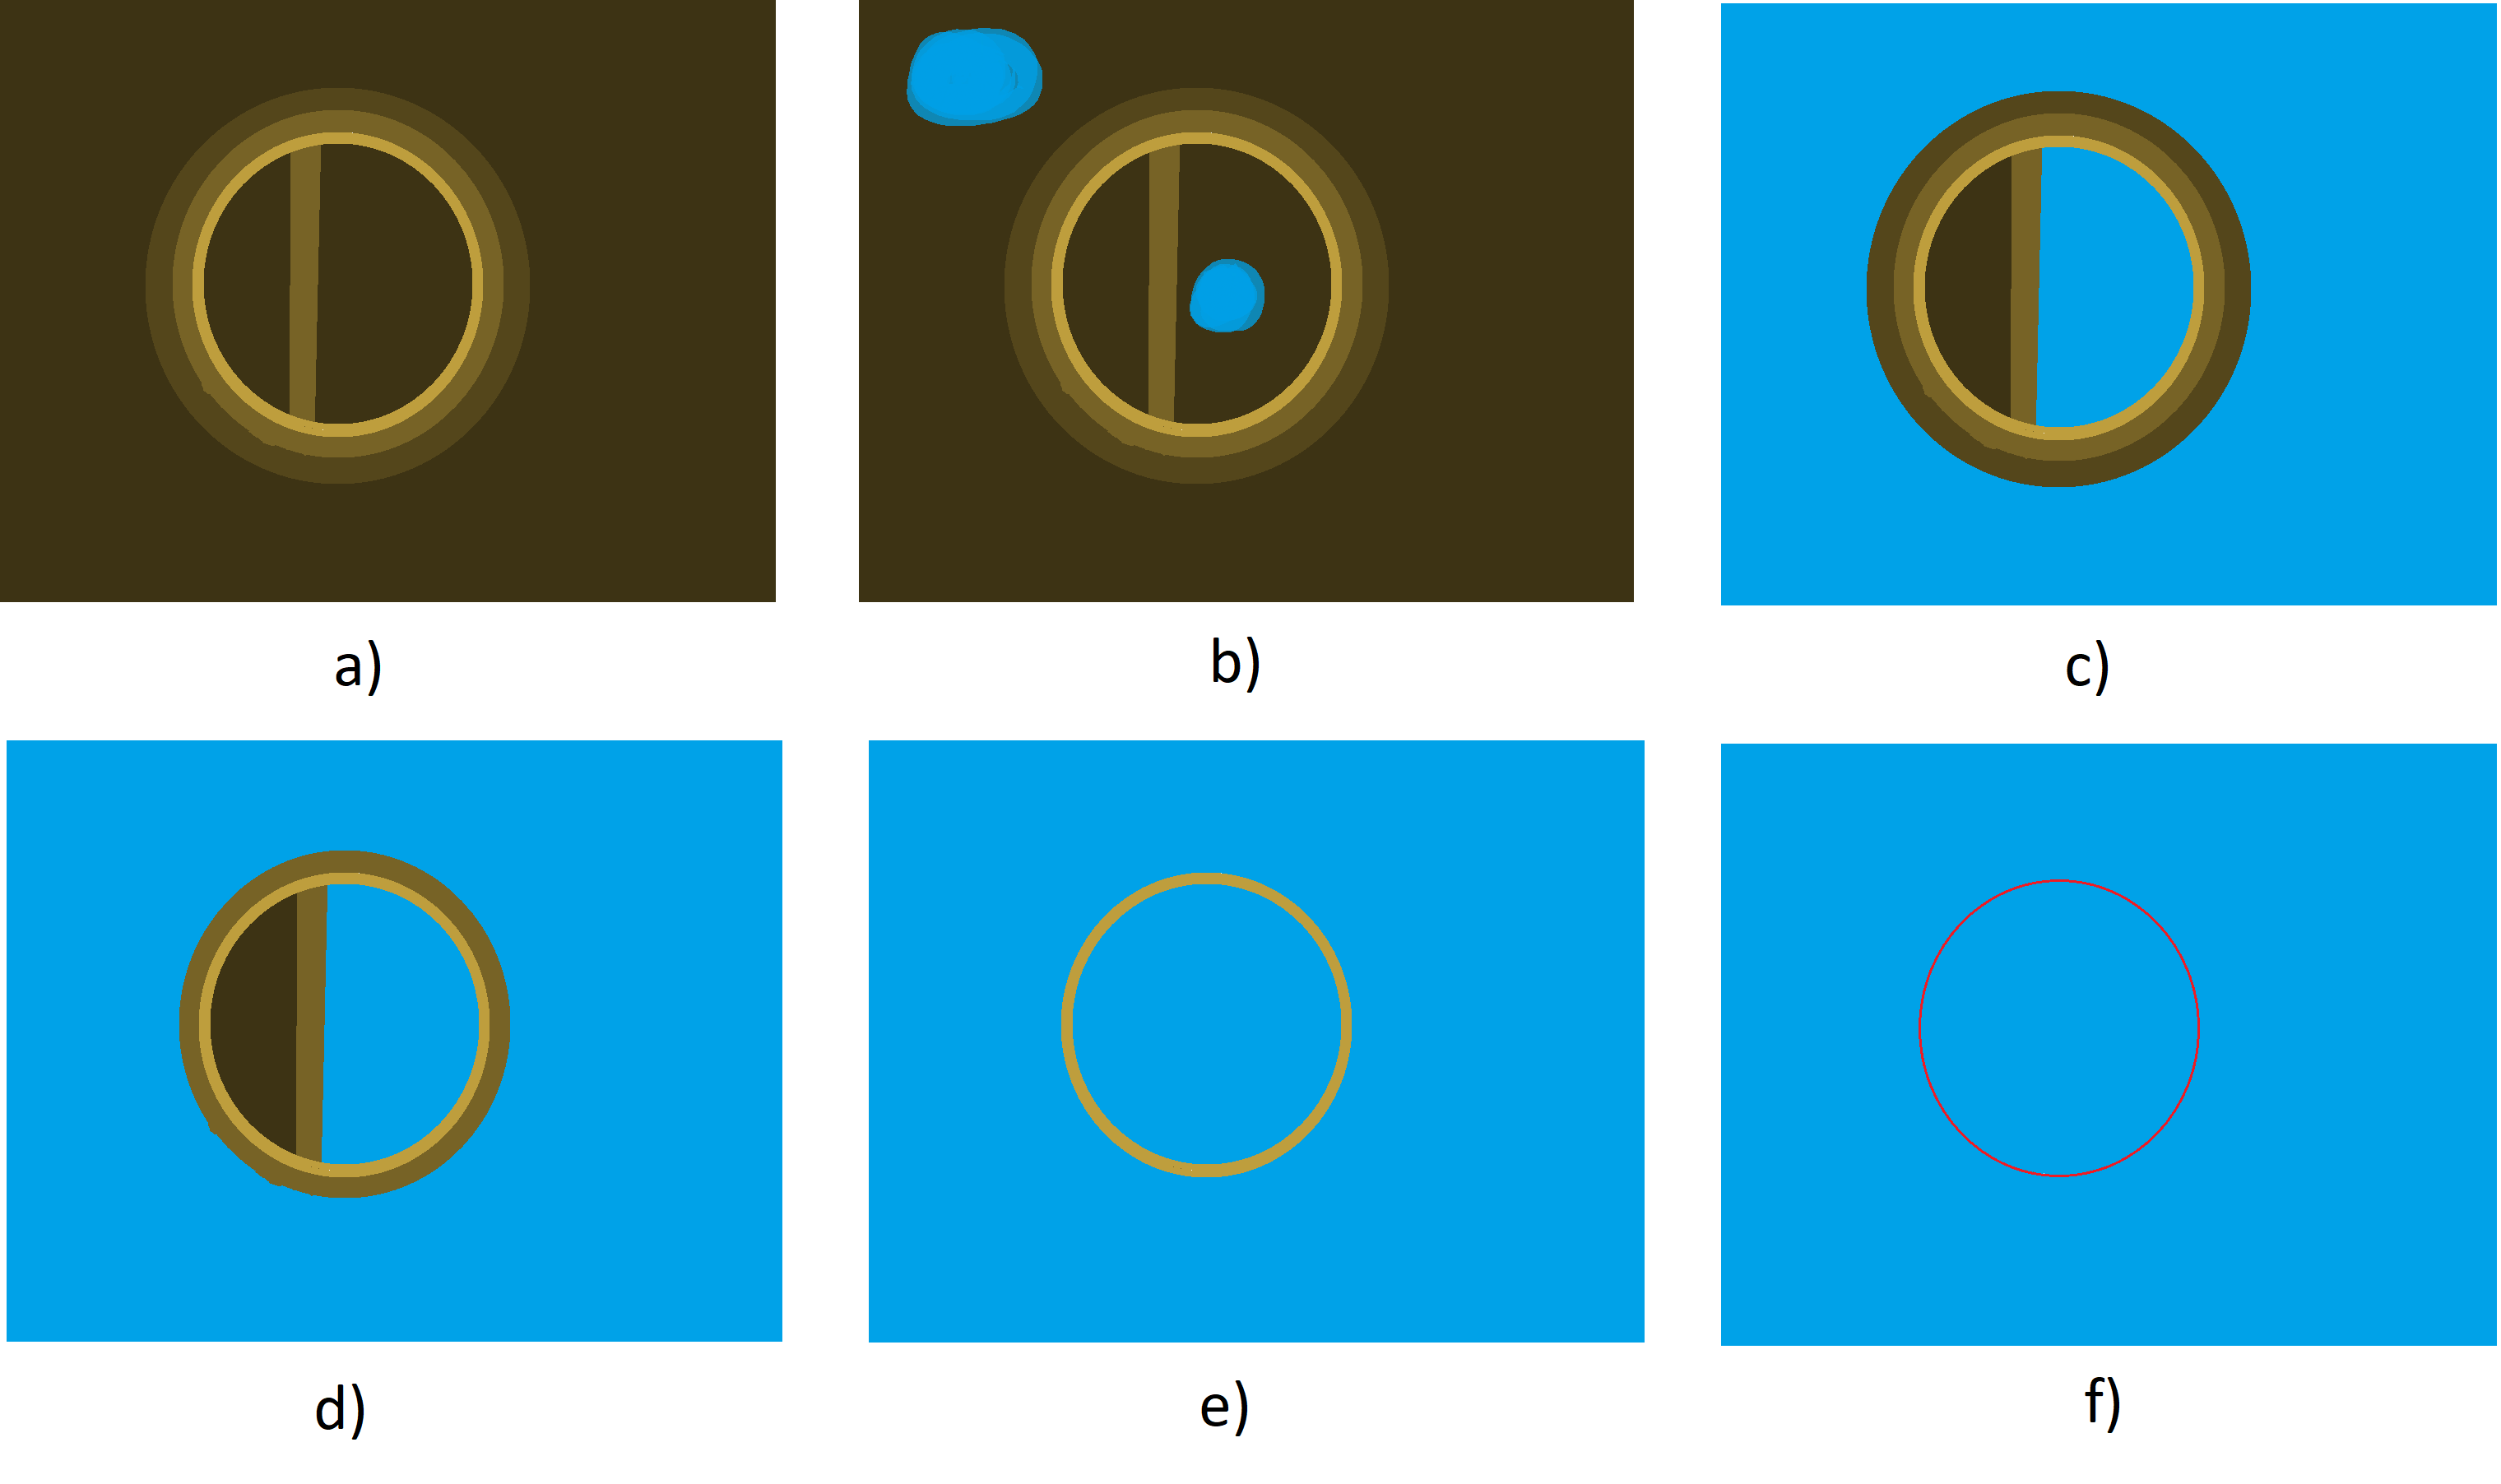
\includegraphics[width=140mm]{./imagenes/con_marcadores.png}
\caption{Proceso de inundación con marcadores del objeto deseado}
\label{img:relieve1}
\end{figure}



\section{Resumen}

En este capítulo se presentan los conceptos de:
\begin{itemize}
\item Segmentación
\item Operaciones básicas de matemática morfológica
\item Dilatación
\item Erosión
\item Gradiente morfológica
\item Criterios de ordenación de colores
\item Trasformada de watershed sin marcadores
\item Sobre-segmentación
\item Trasformada de watershed con marcadores
\end{itemize}
Se ejemplifica el proceso de inundación con y sin marcadores.

% %!TEX root = ../main.tex
\chapter{Transformada watershed por inundación CIELab}
\label{chap:watershed}

%!TEX root = ../main.tex
La propuesta de este trabajo se basa en la extensión del algoritmo de \textit{watershed} en el espacio de color CIELab utilizando la distancia a un punto de referencia. La Figura \ref{img:flujo} muestra el flujo de trabajo propuesto. 
\begin{figure*}[h!]
\centering
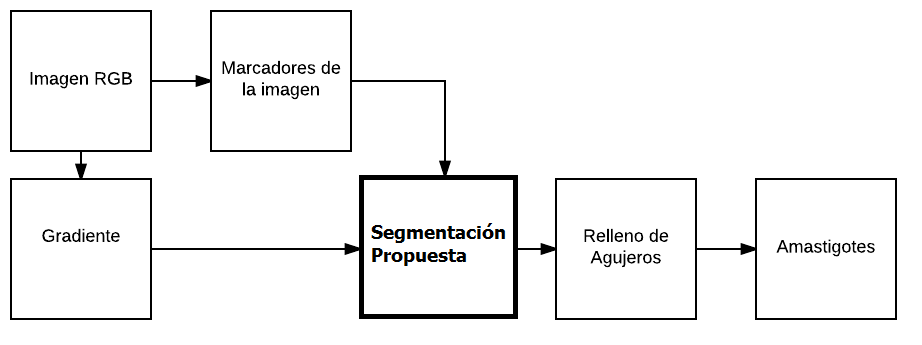
\includegraphics[height=50mm]{./figuras/flujo.png}
\caption{Flujo del trabajo propuesto}
\label{img:flujo}
\end{figure*}
El proceso de la segmentación propuesta está compuesta de varios procesos como se muestran en la Figura \ref{img:segpropuesta}, que se explican posteriormente en el Algoritmo \ref{algoritmo}. 
\begin{figure*}[h!]
\centering
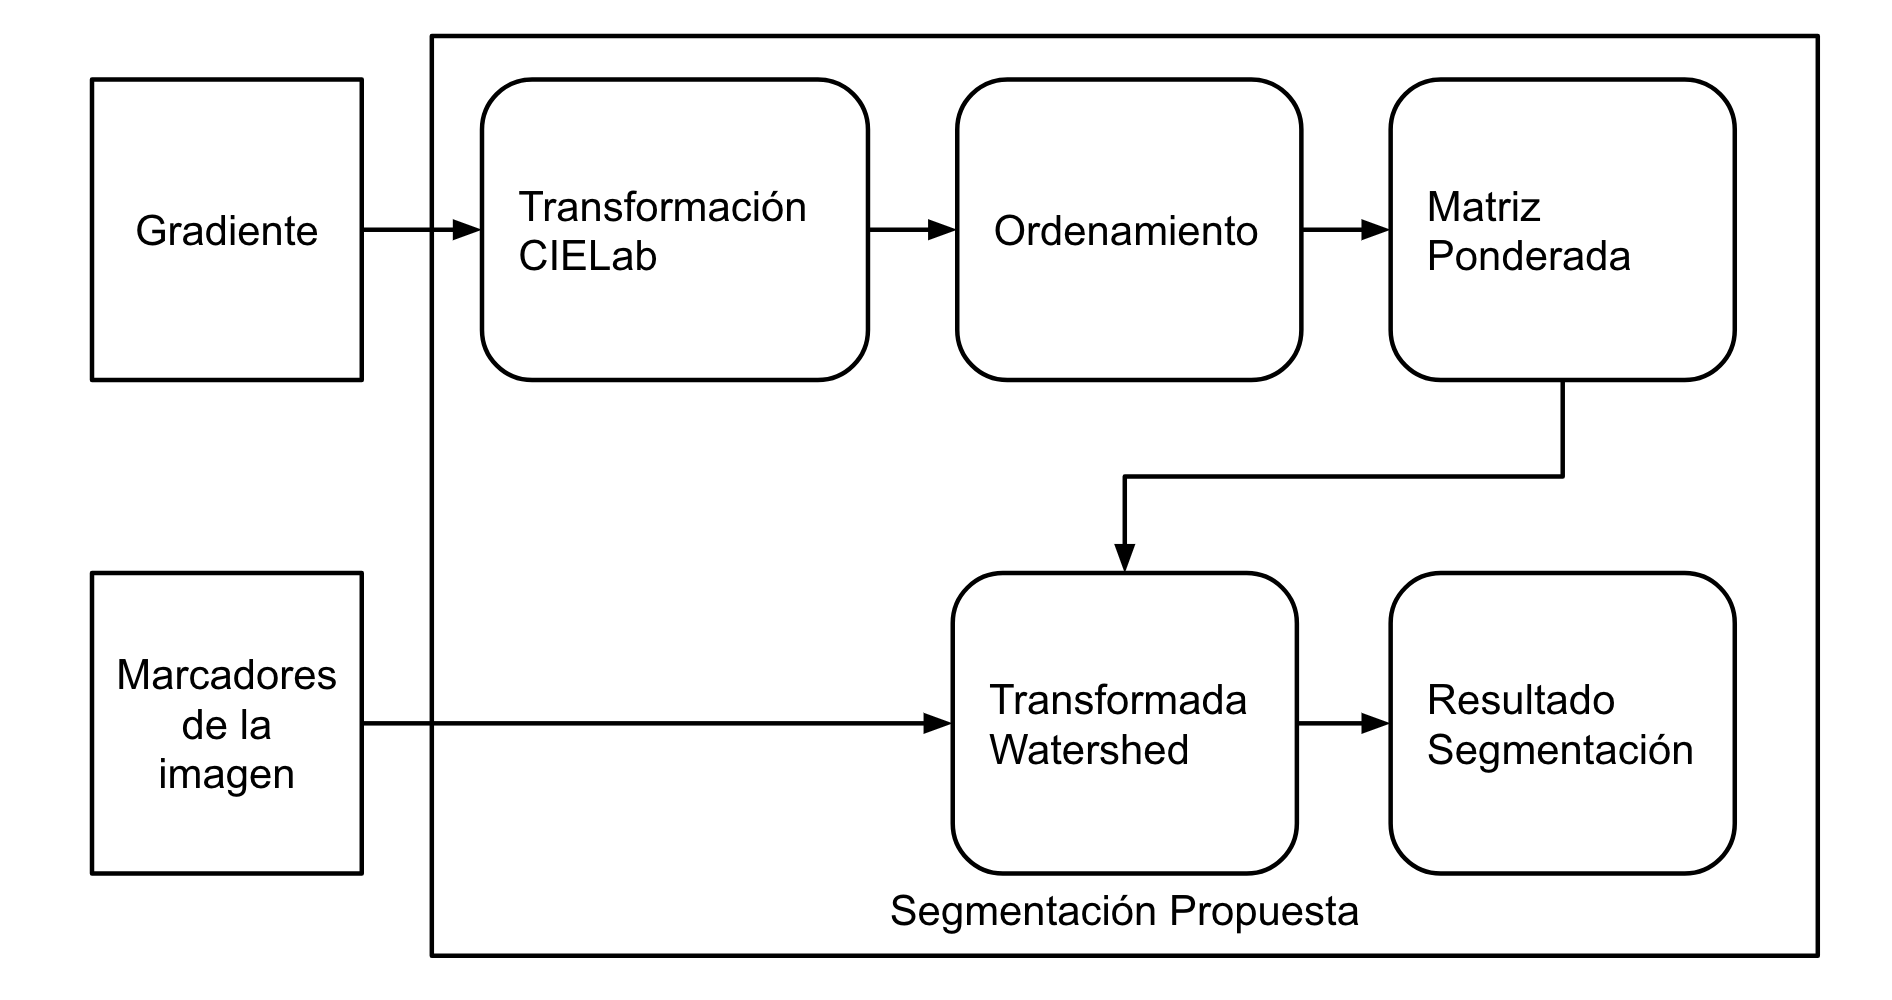
\includegraphics[height=50mm]{./figuras/segmentacion_propuesta.png}
\caption{Flujo de la segmentación propuesta}
\label{img:segpropuesta}
\end{figure*}
\addsymbol{symbol:A}\addsymbol{symbol:B}\addsymbol{symbol:C}
Con el objetivo de ejemplificar el proceso de la segmentación propuesta se utiliza de ejemplo una imagen de tamaño $4 \times 4$. En el Algoritmo \ref{algoritmo} se detallan los pasos a seguir para la realizar la segmentación propuesta de la transformada watershed por inundación con marcadores. Los parámetros de entrada son la gradiente de la imagen y los marcadores como se muestran en la Figura \ref{img:vector-imagen}. A continuación se explica la ejecución del Algoritmo \ref{algoritmo}, donde las variables utilizadas en el texto se encuentran en cursiva para facilitar el seguimiento. 
\begin{figure}[h!]
\centering
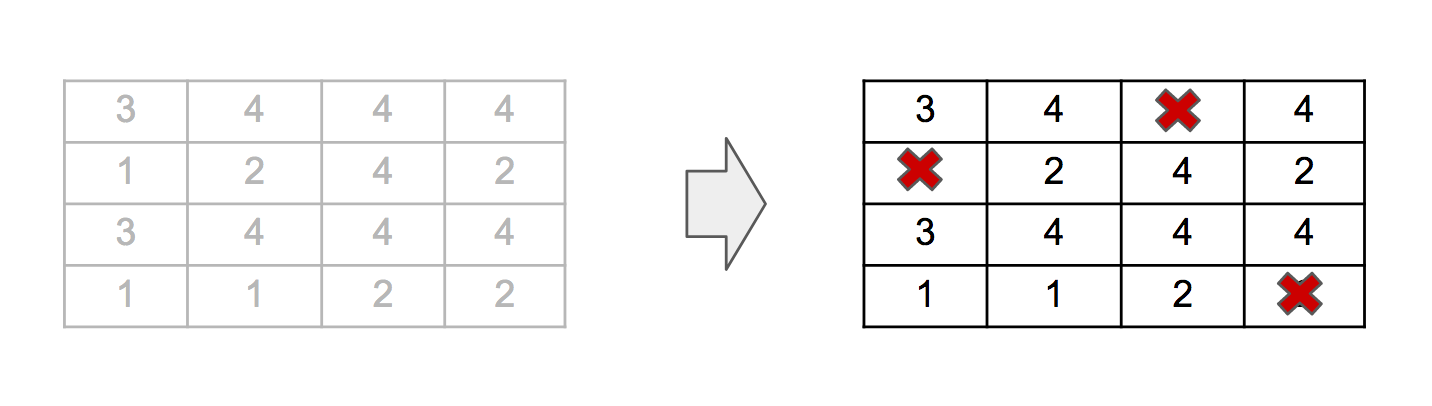
\includegraphics[width=90mm]{./inundacion/inicial.png}
\caption{(a) Gradiente de la imagen, (b) Marcadores de la imagen}
\label{img:vector-imagen}
\end{figure}

Se inicializa una matriz ponderada $transformada$ con los valores por píxel de la transformación de la gradiente del espacio de color RGB a CIELab según la ecuación (\ref{formula:eucli}). En la Figura \ref{img:vector-imagen}(a) se puede ver la representación de la gradiente de una imagen de tamaño $4 \times 4$ en la cual los números representan el valor del píxel luego de asignarle una ponderación basada en el ordenamiento en el espacio de color CIELab.
Los marcadores se colocan en un matriz $marcadores$, con los píxeles (1,3), (2,1) y (4,4). En la Figura \ref{img:vector-imagen}(b) se muestran los marcadores seleccionados de la gradiente de la imagen. 
Para el procesamiento se inicializa una cola de prioridad $lista$ con los marcadores, los cuales son insertados según los valores de la matriz $transformada$ para cada uno de los píxeles en la matriz $marcadores$ como se muestra en la Figura \ref{img:cola-inicio}.
\begin{figure}[h!]
\centering
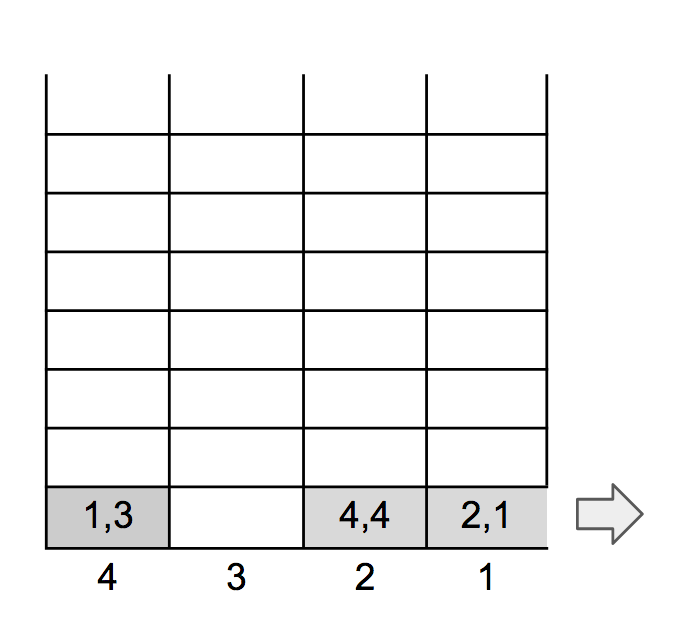
\includegraphics[height=60mm]{./inundacion/cola-inicial.png}
\caption{Inicialización de cola de prioridad}
\label{img:cola-inicio}
\end{figure}
Los píxeles son almacenados en la cola $lista$ de tal forma que el orden (en el cual los píxeles son recuperados de la cola) está dado por dos criterios. El primer criterio esta dado por el nivel en el cual se encuentra el píxel y el segundo está dado por el orden de llegada de los píxeles a su cola. En la Figura \ref{img:prioridad-cola} se muestra una inserción del píxel (2,1) con nivel $1$, teniendo en cuenta los criterios anteriormente citados.
\begin{figure}[h!]
\centering
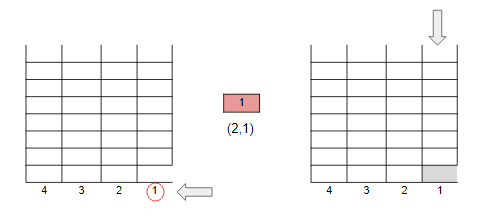
\includegraphics[width=90mm]{./inundacion/prioridad-cola.png}
\caption{(a) Primer criterio de prioridad, (b) Segundo criterio de prioridad}
\label{img:prioridad-cola}
\end{figure}
\SetInd{0.25em}{0.5em}
\renewcommand\bottomfraction{0.85}
\setlength{\textfloatsep}{25pt}
\begin{algorithm2e}
%\setcounter{algocf}{0}% set the counter for the 1st algorithm
\DontPrintSemicolon
%\SetArgSty{textrm}
 \KwIn{Gradiente de la Imagen, Marcadores de la Imagen}
 \KwResult{Imagen Watershed}
  \;
 \Begin{
 Se inicializa una matriz ponderada $transformada$ con los valores por píxel en el espacio de color CIELab según el método de ordenación vectorial reducido con la norma euclidiana.\;
  Se inicializa una matriz $marcadores$ con los marcadores seleccionados.\;
   $lista$ = Cola de prioridad ordenada con los píxeles de $marcadores$ según los valores $transformada[x][y]$.\;
   $pixel$ = $lista.getPixel()$ se obtiene el primer valor de la cola de prioridad.\;
 \Repeat{ $pixel!= NULL$ } {
   $vecinos$ = Se obtienen los vecinos del $pixel$ con conectividad 8.\;
   $posibleEncole$ = Lista para verificar antes de insertar a la $lista$ a procesar.\;
   \ForEach{$vecinos$}{
      \If{$vecino$ no fue procesado} {
      	Se agrega $vecino$ a la lista $posibleEncole$\;
      }
      \If{$vecino$ no está marcado como watershed} {
      	\If{$vecino$ no está marcado} {
      		Se asigna a $pixel$ un nuevo $label$\;
      	}\ElseIf{$vecino$ está marcado con un $label$ distinto a $pixel$}{
      		Se marca el $pixel$ como watershed\;
      	}
      }
   }
   \If{$pixel$ no está marcado como watershed} {
      	Se agrega a $lista$ los píxeles de la lista $posibleEncole$ y se marcan como procesados\;
    }
    \If{$pixel$ no está marcado} {
      	Asignar a $pixel$ el nuevo $label$\;
    }
    $pixel$ = $lista.getPixel()$ se obtiene el siguiente valor de la cola de prioridad.\;
 }
 }
\caption{Segmentación Watershed por Inundación a Color en espacio CIELab}
\label{algoritmo}  
\end{algorithm2e}

El estado inicial de las  etiquetas $A$, $B$ y $C$ para los marcadores mencionados anteriormente, se puede observar en la Figura \ref{img:resultado-inicial} (a). Posteriormente se procesa el primer píxel de la cola de más alta prioridad, en este caso se toma el píxel (2,1), como se puede ver en la Figura \ref{img:cola-inicio}, el cual cuenta con mayor prioridad. 
\begin{figure}[h!]
\centering
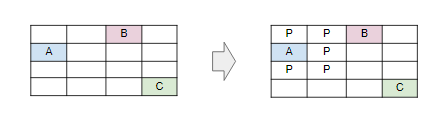
\includegraphics[width=90mm]{./inundacion/resultado-inicial.png}
\caption{(a) Inicialización de etiquetas, (b) Resultado de inundar el píxel (2,1)}
\label{img:resultado-inicial}
\end{figure}
A medida que estos píxeles van siendo procesados, son extraídos de las colas. Dichas colas pueden quedar vacías, lo que implica la eliminación de la misma al momento de la siguiente extracción de píxeles. Por cada $pixel$ extraído, se recorre la lista de $vecinos$ del mismo como se muestran en la Figura \ref{img:cola-vacia} (a), para identificar los que no han sido procesados aún e insertarlos en la cola según el nivel al que corresponde. Los vecinos del píxel en cuestión son analizados antes de incluir a la cola, para ello se utiliza una lista $posibleEncole$ que agrega a la cola todos los vecinos que no hayan sido procesados, pero teniendo en cuenta que el píxel en cuestión no corresponda a las lineas de watershed con la etiqueta $W$. Una vez procesados son marcados con la etiqueta $P$ como se puede observar en la Figura \ref{img:resultado-inicial} (b).
\addsymbol{symbol:P} 
\begin{figure}[h!]
\centering
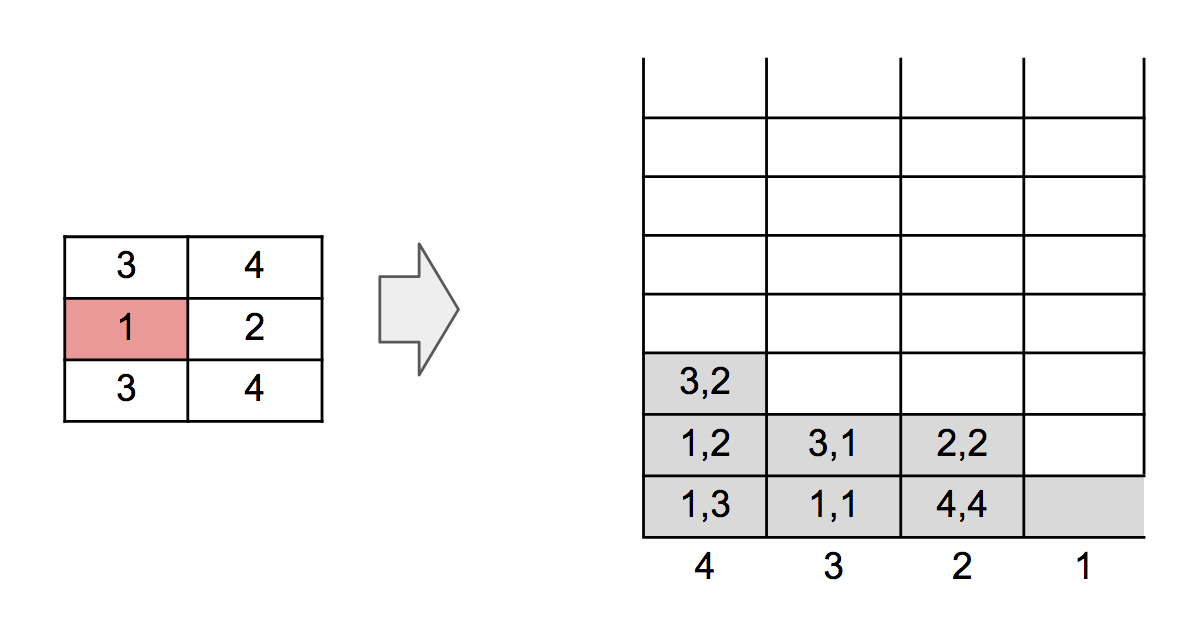
\includegraphics[width=90mm]{./inundacion/cola-vacia.png}
\caption{(a) Vecinos del píxel (2,1), (b) Cola con prioridad mas alta vacía}
\label{img:cola-vacia}
\end{figure}

\begin{figure}[h!]
\centering
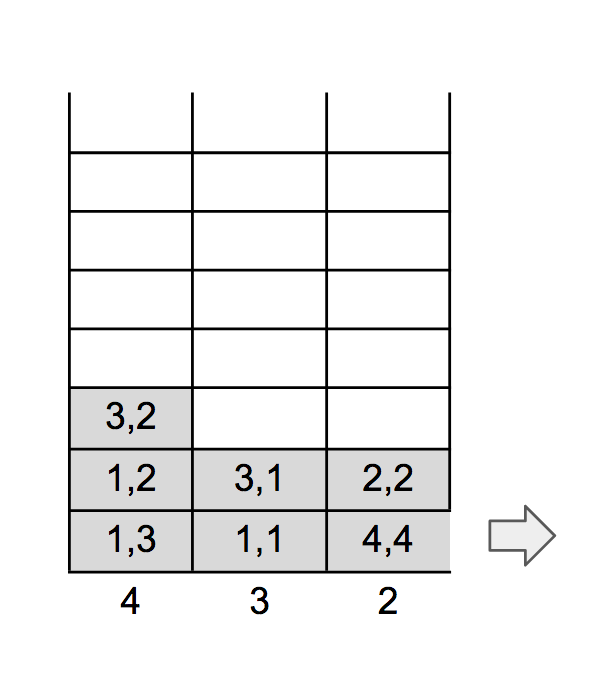
\includegraphics[width=60mm]{./inundacion/cola-eliminada.png}
\caption{Eliminación de cola vacía}
\label{img:cola-eliminada}
\end{figure}

La Figura \ref{img:cola-vacia} (b) muestra el estado de la cola de prioridad luego del procesamiento del píxel (2,1), donde se muestra que la cola de más alta prioridad esta vacía. Cuando un píxel a insertar cuente con una prioridad más alta que la actual, significa que la cola con la prioridad correspondiente ya fue procesada y eliminada, por lo que en dicho caso se debe insertar el píxel en la cola con la prioridad más alta~\cite{Meyer}. En la Figura \ref{img:cola-eliminada} se puede observar que la cola con prioridad 1 ha sido eliminada.
\begin{figure}[h!]
\centering
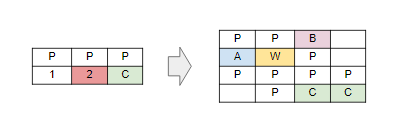
\includegraphics[width=90mm]{./inundacion/unico-label.png}
\caption{(a) Vecinos del píxel (4,4), (b) Etiqueta $C$ asignada en píxel (4,4)}
\label{img:unico-label}
\end{figure}
\begin{figure}[h!]
\centering
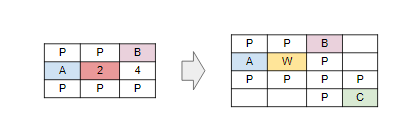
\includegraphics[width=90mm]{./inundacion/varios-label.png}
\caption{(a) Vecinos del píxel (2,2), (b) Etiqueta $W$ asignada en píxel (2,2)}
\label{img:varios-label}
\end{figure}


La etiqueta en una determinada ubicación es determinada de acuerdo a las etiquetas de sus vecinos. En el caso que se cuente solamente con una etiqueta se marca el píxel correspondiente con dicha etiqueta. En la Figura \ref{img:unico-label} (a) se muestran los vecinos del píxel (4,4) y en (b) la asignación de la etiqueta $C$ al píxel (4,4) ya que no existe otra etiqueta diferente. Las vasijas se forman partiendo de los marcadores y se van inundando desde el menor hacia el mayor nivel, según van siendo extraídos de la cola de prioridad. El punto donde se encuentran dos o mas vasijas, es decir, los vecinos cuentan con más de una etiqueta, y no formen parte de la linea de watershed, pasa a formar parte de la linea watershed. En esta ubicación se marca el píxel correspondiente a las lineas de watershed con la etiqueta $W$. 
\addsymbol{symbol:W}
En la Figura \ref{img:varios-label}(a) se muestran los vecinos del píxel (2,2) que poseen etiquetas $A$ y $B$, lo que implica la asignación de la etiqueta W al píxel (2,2) como se muestra en la Figura \ref{img:varios-label}(b).

El proceso se detiene una vez que todos los píxeles de la cola han sido procesados. En la Figura \ref{img:resultado-final} se muestra el estado final de la transformada watershed por inundación.
\begin{figure}[h!]
\centering
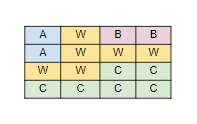
\includegraphics[height=30mm]{./inundacion/resultado-final.png}
\caption{Resultado de la segmentación propuesta}
\label{img:resultado-final}
\end{figure}

A continuación se muestra un ejemplo de la propuesta de este trabajo. Dada una imagen de entrada en RGB como se muestra en la Figura \ref{img:imgprop} se calcula la gradiente marginal, y se seleccionan manualmente los marcadores a ser utilizados para la segmentación.
\begin{figure*}[h!]
\centering
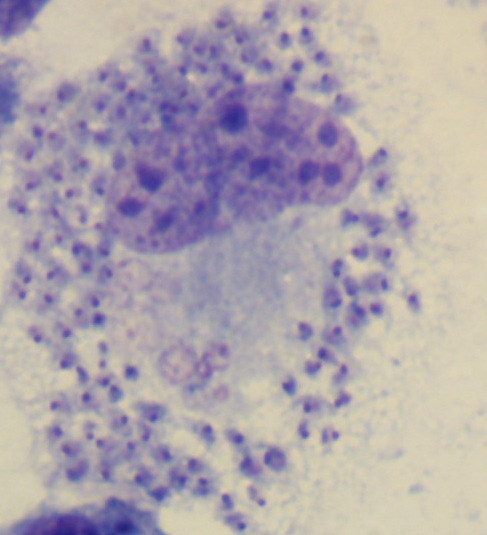
\includegraphics[height=70mm]{./propuesta/cruzi26.jpg}
\caption{Imagen RGB} 
\label{img:imgprop}
\end{figure*}
Los marcadores de la imagen se muestran en La Figura \ref{img:imgmark}, donde se marca manualmente cada uno de los objetos deseados.
\begin{figure}[h!]
\centering
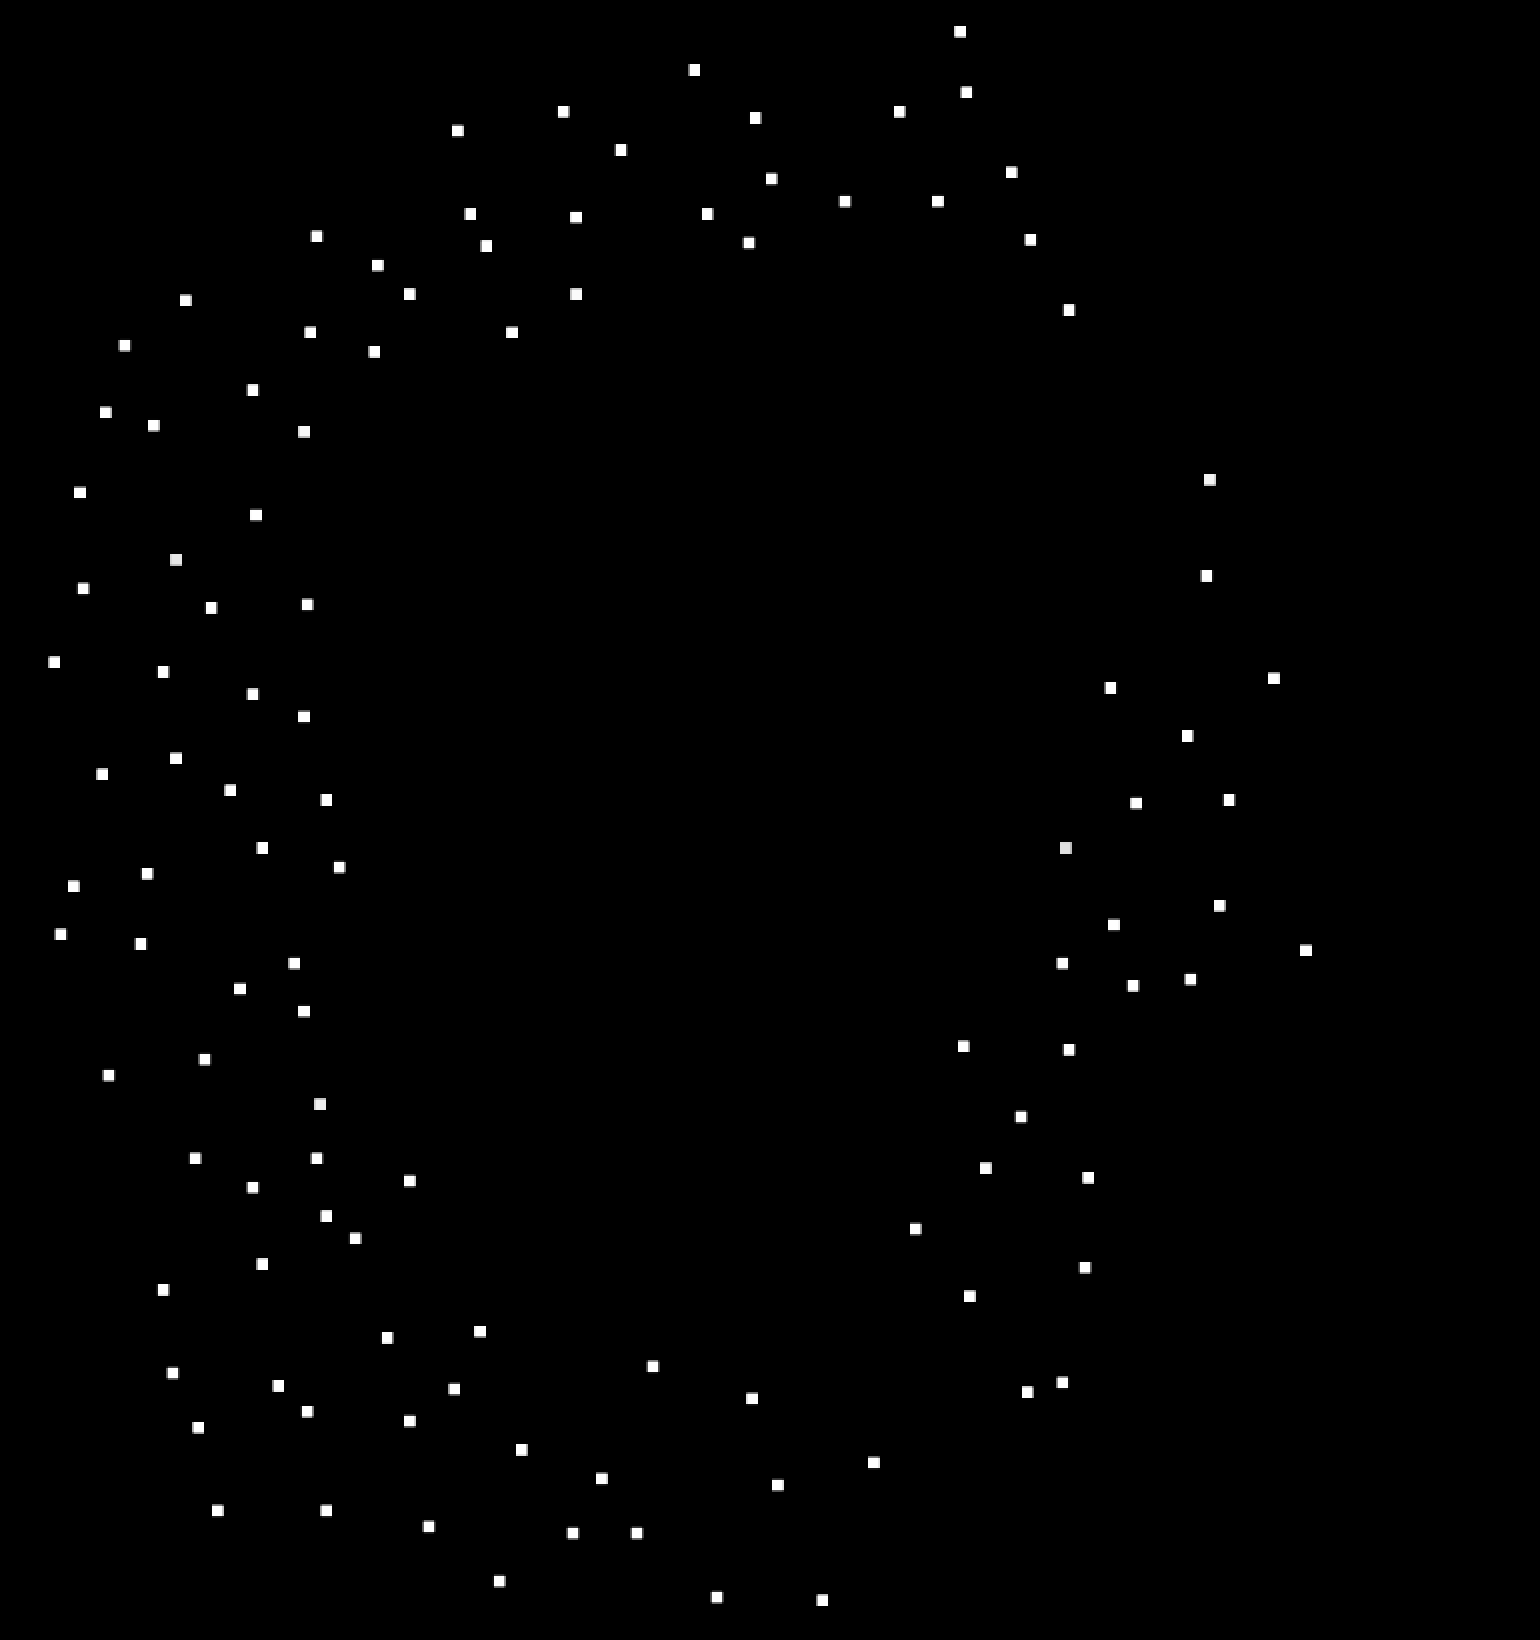
\includegraphics[height=70mm]{./propuesta/marcadores.png}
\caption{Marcadores de la Imagen} 
\label{img:imgmark}
\end{figure}
\begin{figure}[h!]
\centering
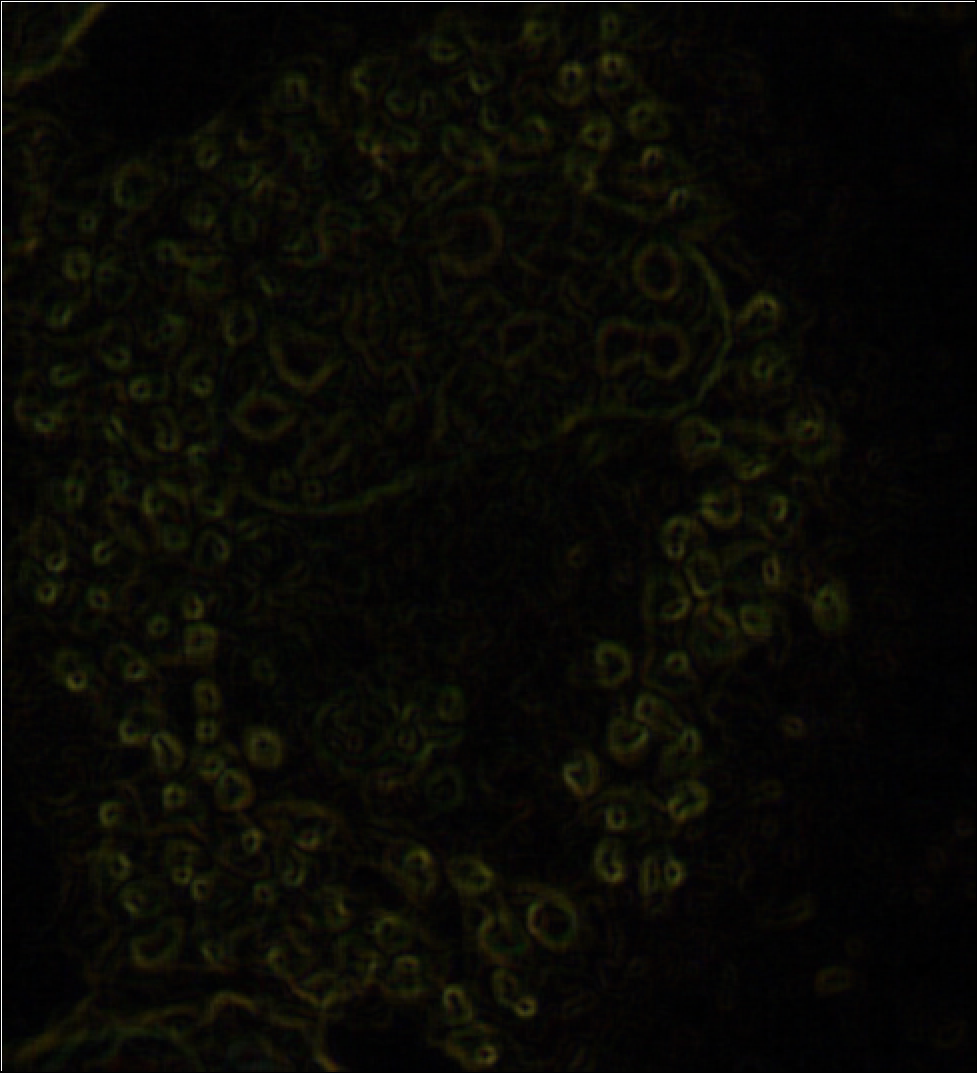
\includegraphics[height=70mm]{./propuesta/gradiente.png}
\caption{Gradiente de la imagen}
\label{img:imggrad}
\end{figure}

La gradiente de la imagen como se muestra en la Figura \ref{img:imggrad} es utilizada para calcular la matriz que será la imagen de entrada para la transformada de watershed. Esta matriz se obtiene calculando para cada píxel un valor escalar que representa el orden en el que se encuentra entre todos los píxeles de la imagen una vez aplicado el ordenamiento  bajo la norma euclidiana según la ecuación (\ref{formula:eucli}). La transformada de watershed utiliza la matriz ponderada y los marcadores pre-seleccionados para realizar la segmentación. 
\begin{figure}[h!]
\centering
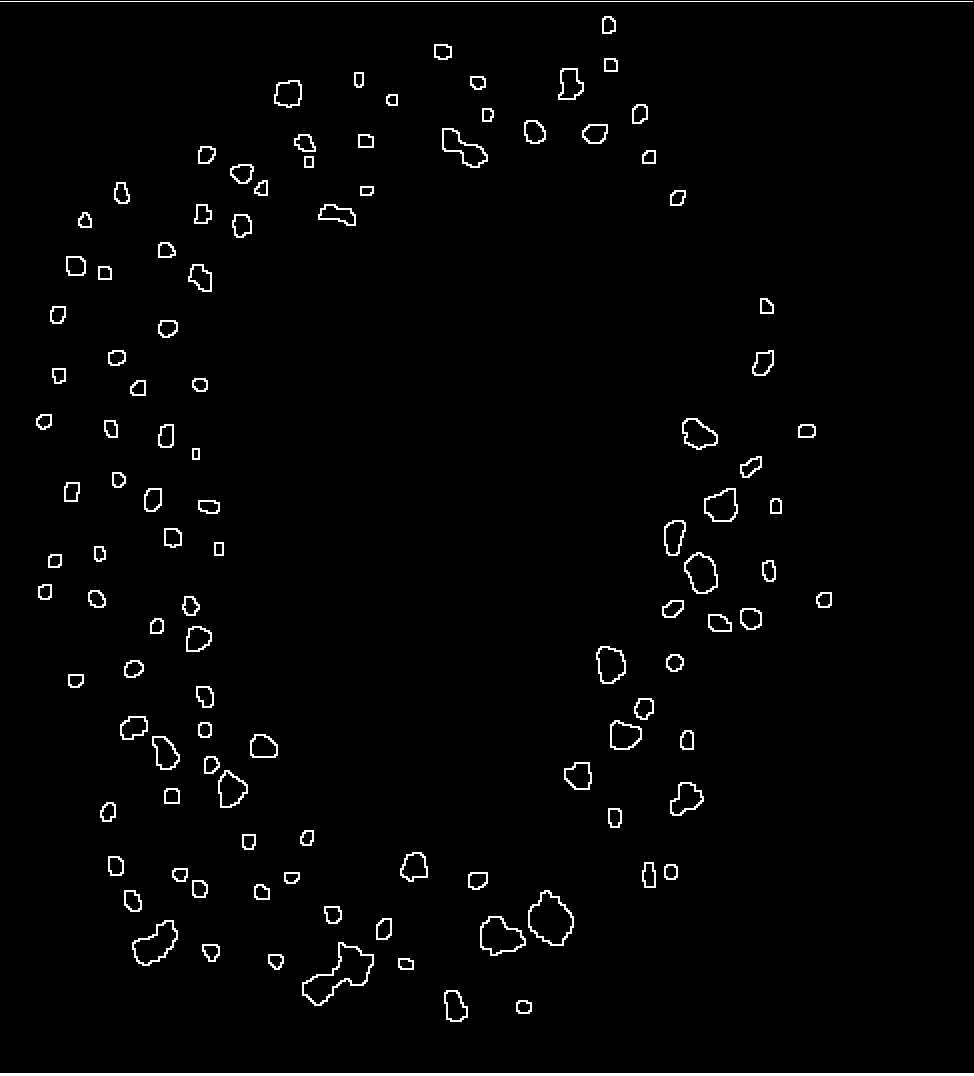
\includegraphics[height=70mm]{./propuesta/relleno.png}
\caption{Resultado de la segmentación de la imagen}
\label{img:imgrelleno}
\end{figure}
\begin{figure*}[h!]
\centering

\includegraphics[height=70mm]{./propuesta/resultado.png}
\caption{Resultado de la propuesta de este trabajo}
\label{img:imgresultado}
\end{figure*}
El resultado de la propuesta de este trabajo se muestra en la Figura \ref{img:imgrelleno}, donde están presentes los contornos de los objetos, sobre el cual se aplica un rellenado de agujeros para su mejor visualización, como se puede observar en la Figura \ref{img:imgresultado}. El proceso de relleno de agujeros se encuentra facilitado por el hecho que los resultados contienen objetos cerrados. Este proceso se realiza buscando dichos objetos de izquierda a derecha y posteriormente de arriba a abajo, rellenando así todo su trayecto desde el inicio hasta el final de cada objeto encontrado.
\begin{figure*}[h!]
\centering

\includegraphics[height=70mm]{./propuesta/amastigotes.jpg}
\caption{Amastigotes segmentados}
\label{img:imgamastigotes}
\end{figure*}

Posteriormente se tiene como resultado final los amastigotes de Trypanosoma cruzi segmentados, como se puede ver en la Figura \ref{img:imgamastigotes}. Los amastigotes segmentados en algunos casos pueden ser más grandes o más pequeños, donde el tamaño ideal de los mismos, el cual es utilizado para la comparación, fue determinado por un especialista. En algunos casos se puede observar que dos o más amastigotes son segmentados como si fuera solo uno. La cuantificación numérica de los resultados para todos los casos obtenidos serán presentados mediante las métricas de evaluación descritas en el próximo capítulo.

\section{Resumen}

En este capítulo se presentó la propuesta del trabajo, el funcionamiento del algoritmo de watershed propuesto por Vincent y Soille y el enfoque de como extenderlo en imágenes a color. El proceso de relleno de agujeros para mejorar la visualización de los resultados fue explicado, mostrando además un ejemplo con imágenes del caso de estudio en algunos de los estados mas importantes del algoritmo.

% %!TEX root = ../tesis.tex
\chapter{Resultados}
\label{chap:resultados}

En este capítulo se definen las métricas utilizadas para la evaluación de la extensión de la transformada de watershed implementada y se presentan los resultados obtenidos en los experimentos.

\section{Métricas de Evaluación}
El objetivo de la segmentación es separar los objetos deseados del fondo para el estudio futuro~\cite{carrasco}. A partir de los objetos segmentados se pueden clasificar los píxeles en cuatro resultados posibles:
\addsymbol{symbol:VP} \addsymbol{symbol:VN} 
\addsymbol{symbol:FP} \addsymbol{symbol:FN} 
\begin{itemize}
\item Verdadero Positivo ($VP$), píxel que pertenece al objeto segmentado y es segmentado como tal.
\item Falso Positivo ($FP$), píxel que no pertenece al objeto segmentado y es segmentado como parte del mismo erróneamente.
\item Verdadero Negativo ($VN$), píxel que no pertenece al objeto segmentado y no es segmentado como parte del mismo.
\item Falso Negativo ($FN$), píxel que pertenece al objeto segmentado y no es segmentado como tal.
\end{itemize}
La clasificación de los resultados obtenidos para las distintas variables se puede observar en la Figura \ref{img:vpfp}. Las zonas en donde el objeto a segmentar y la segmentación realizada se interceptan corresponde a los píxeles considerados como $VP$, en donde el objeto no intercepta a la segmentación realizada corresponde a los $FN$. Posteriormente los píxeles que son parte de la segmentación realizada pero no el objeto son los $FP$ y los píxeles del fondo de la imagen que si corresponden al fondo son los $VN$.
\begin{figure}[H]
\centering
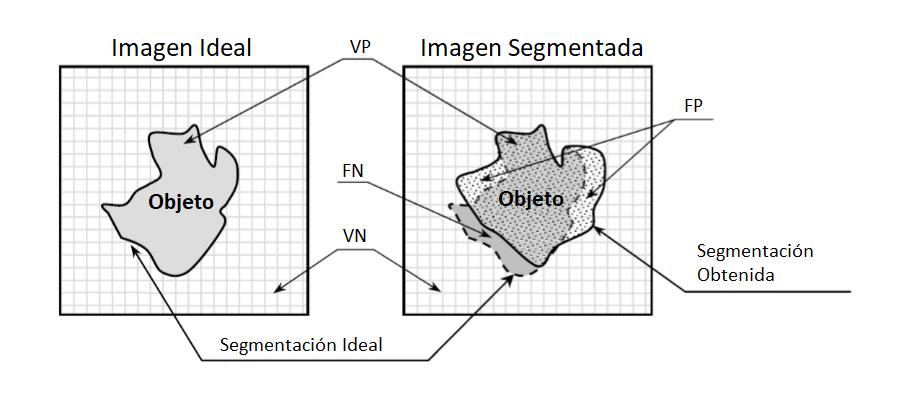
\includegraphics[width=160mm]{./imagenes/metricas-imagen.png}
\caption{Resultados posibles de la segmentación}
\label{img:vpfp}
\end{figure}
Para el problema estudiado la imagen ideal representa la segmentación hecha por un profesional, y la imagen segmentada representa la segmentación de los amastigotes obtenidos automáticamente. Se puede considerar que los $VP$ son los píxeles que pertenecen al amastigote y fueron segmentados correctamente, los $FP$ son los píxeles que fueron segmentados como parte de el amastigote pero no lo son, los $FN$ son los píxeles que forman parte del amastigote pero no fueron segmentados como tal y los $VN$ son los píxeles que forman parte del fondo y fueron segmentados correctamente.

Para la comparación de los resultados obtenidos, se utilizan las siguientes métricas:
\begin{itemize}
\item Sensibilidad ($SEN$): La probabilidad de segmentar correctamente un amastigote.
\begin{equation}\label{eq:sensibilidad}
  SEN = \cfrac{VP}{VP + FN}.
\end{equation}
\item Especificidad ($ESP$): La probabilidad de segmentar correctamente el fondo.
\begin{equation}\label{eq:especificidad}
  ESP = \cfrac{VN}{VN + FP}.
\end{equation}
\item Exactitud ($EX$): La probabilidad de que un amastigote o el fondo obtengan una segmentación correcta.
\begin{equation}\label{eq:exactitud}
  EX = \cfrac{VP + VN}{VP + VN + FP + FN}.
\end{equation}
\end{itemize}
%!TEX root = ../tesis.tex
\section{Experimentos}
Para los experimentos se utilizó una base de datos con 100 imágenes microscópicas de células infectadas con amastigotes de Trypanosoma Cruzi~\cite{noguera2013mathematical}.

Los diferentes órdenes  utilizados se muestran en la Tabla \ref{metodos-ordenamiento}. Los métodos propuestos son los que utilizan la distancia a un color de referencia en el espacio de color CIELab, en nuestro caso se propuso la utilización de la distancia euclidiana al color origen, media y mediana de la imagen. Para las imágenes en escala de grises se utilizó el orden natural entre las intensidades de los píxeles, en el espacio de color HSI se utilizó el orden lexicográfico y en el espacio de color RGB se utilizaron los órdenes lexicográfico, alpha-lexicográfico, el ordenamiento propuesto por Meyer y los ordenamientos propuesto por Vázquez.

\begin{table}[]
\centering
\caption{Métodos de ordenamiento}
\label{metodos-ordenamiento}
\resizebox{15cm}{!} {
\begin{tabular}{|l|l|l|}
\hline
\multicolumn{1}{|c|}{\textbf{Método}} & \multicolumn{1}{c|}{\textbf{Espacio de color}} & \multicolumn{1}{c|}{\textbf{Observación}}  \\ \hline
\textbf{MEDIANA-CIELAB} & CIELab & Espacio propuesto \\ \hline
\textbf{MEDIA-CIELAB} & CIELab & Espacio propuesto \\ \hline
\textbf{DISTANCIA-EUCLIDIANA-CIELAB} & CIELab & Espacio propuesto \\ \hline
\textbf{LEXICOGRAFICO-RGB} & RGB & Sección \ref{chap:marco-lex} \\ \hline
\textbf{ALGORITMO-MEYER} & RGB & Sección \ref{chap:marco-meyer} \\ \hline
\textbf{ALPHA-MOD-LEXICOGRAFICO-RGB} & RGB & Sección \ref{chap:marco-alphalex} \\ \hline
\textbf{DISTANCIA-EUCLIDIANA-RGB} & RGB & Sección \ref{chap:marco-distanciaeuclidianta} \\ \hline
\textbf{ESCALA-DE-GRISES} & Escala de Gris & Sección \ref{chap:marco-lex}  \\ \hline
\textbf{VAZQUEZ-ET-AL} & RGB & Sección \ref{chap:marco-lex} \\ \hline
\textbf{ENTRELAZADO-RGB} & RGB & Sección \ref{chap:marco-entrelazado} \\ \hline
\textbf{LEXICOGRAFICO-HSI} & HSI & Sección \ref{chap:marco-lex} \\ \hline
\textbf{ENTROPIA-RGB} & RGB & Sección \ref{chap:marco-vazquez}  \\ \hline
\textbf{MAXIMO-RGB} & RGB & Sección \ref{chap:marco-vazquez}  \\ \hline
\textbf{MINIMO-RGB} & RGB & Sección \ref{chap:marco-vazquez} \\ \hline
\textbf{MODA-RGB} & RGB & Sección \ref{chap:marco-vazquez}  \\ \hline
\textbf{MODA-MAXIMO-RGB} & RGB & Sección \ref{chap:marco-vazquez} \\ \hline
\textbf{MODA-MINIMO-RGB} & RGB & Sección \ref{chap:marco-vazquez}  \\ \hline
\textbf{SUAVIDAD-RGB} & RGB & Sección \ref{chap:marco-vazquez} \\ \hline
\textbf{VARIANZA-RGB} & RGB & Sección \ref{chap:marco-vazquez}   \\ \hline
\end{tabular}
}
\end{table}


\section{Resultados Obtenidos}
\label{chap:resultados}

En esta sección se brinda un resumen de los resultados obtenidos al realizar los experimentos y se presentan ejemplos visuales de los experimentos.

\subsection{Resultados numéricos}

A continuación se muestran los resultados promedios obtenidos para los $VP$, $FP$, $VN$ y $FN$ en la Tabla \ref{resultados} (Ver resultados de manera extensiva en el Anexo \ref{chap:ApendiceA}). Los valores presentados muestran que el ordenamiento \textbf{MEDIANA-CIELAB} obtuvo los mayores resultados para las cuatro variables a considerar. En todos los resultados para los distintos métodos existe una gran cantidad de $FP$, esto indica que al realizar la segmentación los objetos obtenidos son de un tamaño mayor a los objetos en la imagen ideal. En los resultados se observa también que los métodos \textbf{MEDIANA-CIELAB} y \textbf{MEDIA-CIELAB} fueron los únicos que obtuvieron una cantidad mayor al 40\% en $VP$ por lo cual la distancia a colores de referencia que utilizan información de la imagen, como la mediana y la media, son los más adecuados para la segmentación de los amastigotes de Trypanosoma Cruzi.

\begin{table*}[]
\centering
\caption{Resultados de la Comparación}
\label{resultados}
\resizebox{15cm}{!} {
\begin{tabular}{|l|l|l|l|l|}
\hline
\multicolumn{1}{|c|}{\textbf{Método}} & \multicolumn{1}{c|}{\textbf{FP}} & \multicolumn{1}{c|}{\textbf{VP}} & \multicolumn{1}{c|}{\textbf{FN}}	&	\multicolumn{1}{c|}{\textbf{VN}} \\ \hline
\textbf{MEDIANA-CIELAB} & 53.9871 & 46.0129 & 3.241 & 96.759\\ \hline
\textbf{MEDIA-CIELAB} & 58.0464 & 41.9536 & 3.8889 & 96.1111\\ \hline
\textbf{DISTANCIA-EUCLIDIANA-CIELAB} & 62.382 & 37.618 & 3.388 & 96.612\\ \hline
\textbf{LEXICOGRAFICO-RGB} & 62.5968 & 37.4032 & 4.5841 & 95.4159\\ \hline
\textbf{ALGORITMO-MEYER} & 61.9621 & 38.0379 & 4.2933 & 95.7067 \\ \hline
\textbf{ALPHA-MOD-LEXICOGRAFICO-RGB} & 64.4714 & 32.6382 & 4.7328 & 95.2672\\ \hline
\textbf{DISTANCIA-EUCLIDIANA-RGB} & 64.4714 & 35.5286 & 4.6877 & 95.3123 \\ \hline
\textbf{ESCALA-DE-GRISES} & 62.4645 & 37.5355 & 4.9666 & 95.0334 \\ \hline
\textbf{VAZQUEZ-ET-AL} & 66.7119 & 33.2881 & 4.8933 & 95.1067\\ \hline
\textbf{ENTRELAZADO-RGB} & 67.171 & 32.829 & 5.5399 & 94.4601 \\ \hline
\textbf{LEXICOGRAFICO-HSI} & 65.1106 & 34.8894 & 5.6917 & 94.3083 \\ \hline
\textbf{ENTROPIA-RGB} & 66.6292 & 33.3708 & 5.5686 & 94.4314 \\ \hline
\textbf{MAXIMO-RGB} & 67.0666 & 32.9334 & 5.0553 & 94.9447 \\ \hline
\textbf{MINIMO-RGB} & 65.8297 & 34.1703 & 5.6771 & 94.3229 \\ \hline
\textbf{MODA-RGB} & 64.8527 & 35.1473 & 4.6959 & 95.3041 \\ \hline
\textbf{MODA-MAXIMO-RGB} & 64.8527 & 35.1473 & 4.6959 & 95.3041 \\ \hline
\textbf{MODA-MINIMO-RGB} & 64.8527 & 35.1473 & 4.6959 & 95.3041 \\ \hline
\textbf{SUAVIDAD-RGB} & 67.6638 & 32.3362 & 4.4133 & 95.5867 \\ \hline
\textbf{VARIANZA-RGB} & 66.7964 & 33.2036 & 4.8919 & 95.1081 \\ \hline
\end{tabular}
}
\end{table*}

La comparación de las métricas de sensibilidad, exactitud y especificidad de la implementación utilizando distintos métodos de orden entre píxeles, se puede observar en la Tabla \ref{resultadosCielab}. Los valores indican el promedio obtenido por cada método de ordenamiento para todas las imágenes.El método \textbf{MEDIANA-CIELAB} presenta una mejora de 3.14\% en Especificidad y 1.34\% en Exactitud en comparación con el siguiente mejor método. 


\begin{table}[]
\centering
\caption{Resultados en espacio de color CIELab}
\label{resultadosCielab}
\resizebox{15cm}{!} {
\begin{tabular}{|l|l|l|l|}
\hline
\multicolumn{1}{|c|}{\textbf{Método}} & \multicolumn{1}{c|}{\textbf{$SEN$}}& \multicolumn{1}{c|}{\textbf{$ESP$}}&  \multicolumn{1}{c|}{\textbf{$EX$}}  \\ \hline
\textbf{MEDIANA-CIELAB} & 26.18\%  & 93.19\%  & 91.14\%  \\ \hline
\textbf{MEDIA-CIELAB} & 27.14\%  & 92.95\% & 90.94\%  \\ \hline
\textbf{DISTANCIA-EUCLIDIANA-CIELAB} & 27.24\%  & 91.76\% & 89.80\% \\ \hline
\textbf{LEXICOGRAFICO-RGB} & 27.41\%  & 90.05\% & 88.17\% \\ \hline
\textbf{ALGORITMO-MEYER} & 27.02\%  & 90.40\%  & 88.48\% \\ \hline
\textbf{ALPHA-MOD-LEXICOGRAFICO-RGB} & 27.31\% & 89.14\% & 87.27\% \\ \hline
\textbf{DISTANCIA-EUCLIDIANA-RGB} & 27.40\% & 88.73\% & 86.8\%  \\ \hline
\textbf{ESCALA-DE-GRISES} & 25.5\%  & 88.69\%  & 86.81\%  \\ \hline
\textbf{VAZQUEZ-ET-AL} & 27.37\%  & 88.08\%  & 86.25\% \\ \hline
\textbf{ENTRELAZADO-RGB} & 27.27\% & 88.02\% & 86.17\% \\ \hline
\textbf{LEXICOGRAFICO-HSI} & 27.39\%  & 87.96\% & 86.15\%  \\ \hline
\textbf{ENTROPIA-RGB} & 27.24\%  & 87.53\%  & 85.73\% \\ \hline
\textbf{MAXIMO-RGB} & 27.36\%  & 87.40\%  & 85.62\%  \\ \hline
\textbf{MINIMO-RGB} & 27.53\%  & 87.95\%  & 86.15\%  \\ \hline
\textbf{MODA-RGB} & 27.48\%  & 89.03\%  & 87.15\% \\ \hline
\textbf{MODA-MAXIMO-RGB} & 27.48\%  & 89.03\% & 87.15\%   \\ \hline
\textbf{MODA-MINIMO-RGB} & 27.48\%  & 89.03\% &  87.15\%   \\ \hline
\textbf{SUAVIDAD-RGB} & 27.55\% & 88.17\%  & 86.34\% \\ \hline
\textbf{VARIANZA-RGB} & 27.47\%  & 88.17\%  & 86.34\% \\ \hline
\end{tabular}
}
\end{table}

Para obtener un detalle de los datos se contabilizó además la cantidad total de imágenes en las que cada espacio (3 métodos en CIELab, 14 métodos en RGB y 1 método en HSI) de color obtuvo el mejor exactitud (ver Figura \ref{exp:exactitud}). En este conteo se puede ver que el espacio de color CIELab obtuvo la mejor segmentación en la mayor cantidad de las imágenes.

\begin{figure}[h!]
\centering
\includegraphics[width=160mm]{./imagenes/exactitud.png}
\caption{Cantidad de imágenes que dan el mejor resultado en exactitud por método}
\label{exp:exactitud}
\end{figure}

\subsection{Resultados visuales}

A continuación se muestran los ejemplos visuales de los experimentos realizados en el trabajo. La Figura \ref{exp:lab} muestra los resultados obtenidos en el espacio de color CIELab. En la Figura \ref{exp:lab}(a) se muestra una imagen del caso de estudio. Además se muestra la gradiente en la Figura \ref{exp:lab}(b) utilizada para la segmentación. La segmentación obtenida en la Figura \ref{exp:lab}(c) y la segmentación ideal se muestran en la Figura \ref{exp:lab} (d). Este ejemplo será utilizado posteriormente para la comparación con los distintos experimentos realizados.

\begin{figure}[h!]
\centering
\includegraphics[width=150mm]{./imagenes/ejemplo-medialab.png}
\caption{Resultados obtenidos en el espacio de Color CIELab}
\label{exp:lab}
\end{figure}

\subsubsection{Comparación con imágenes en escala de grises}

Los resultados de la implementación utilizando el algoritmo de Vincent y Soille en escala de grises en la Figura \ref{exp:gris} muestran como los amastigotes segmentados en la esquina inferior izquierda en \ref{exp:gris}(c) poseen un tamaño mayor a lo que se ve en la segmentación ideal y en comparación con la segmentación realizada en el espacio CIELab.
\begin{figure}[h]
\centering
\includegraphics[width=150mm]{./imagenes/ejemplo-gris.png}
\caption{Resultados obtenidos utilizando el algoritmo de Vincent y Soille}
\label{exp:gris}
\end{figure}

En base a un análisis visual de los resultados se nota que los amastigotes segmentados tienden a ser de mayor tamaño que los esperados en la imagen ideal, esta tendencia se mantiene tanto en escala de gris como en CIELab pero en este último espacio se ve un tamaño más cercano a la imagen ideal, esto refleja la tendencia obtenida en las tablas anteriores.

\subsubsection{Comparación con imágenes a color}

Los resultados de la implementación utilizando el algoritmo de Meyer en el espacio de color RGB se pueden observar en la Figura \ref{exp:rgb}. 
\begin{figure}[h]
\centering
\includegraphics[width=150mm]{./imagenes/ejemplo-rgb.png}
\caption{Resultados obtenidos utilizando el algoritmo de Meyer}
\label{exp:rgb}
\end{figure}

Realizando un análisis visual de los resultados se puede ver que presenta la misma tendencia que al realizar la segmentación en escala de grises o en el espacio CIELab. Los amastigotes segmentados poseen un tamaño mayor al esperado en la imagen ideal así como lo indica la alta presencia de $FP$ en los resultados numéricos.

Comparando con los resultados obtenidos en escala de grises se puede ver una mejora al utilizar el color y comparando con la segmentación en el espacio de color CIELab se puede ver un resultado similar, tomando los amastigotes segmentados en la esquina inferior izquierda existe un mayor error de incremento de tamaño en el espacio de color RGB en comparación con el espacio de color CIELab.


En la Figura \ref{img:r1}(a) se muestra la imagen original y en \ref{img:r1}(b) la segmentación ideal.

\begin{figure}[H]
\centering
\includegraphics[width=100mm]{./imagenes/r1.png}
\caption{(a) Imagen original (b) Segmentación ideal}
\label{img:r1}
\end{figure}

En la Figura \ref{img:r2}(a) se muestra la segmentación obtenida en el espacio CIELab con el ordenamiento de la distancia a la mediana y en la Figura \ref{img:r2}(b) el espacio RGB utilizando el ordenamiento lexicógrafo, el cual obtuvo los mejores resultados entre los distintos espacios de color y ordenamientos que no utilizan el espacio CIELab. Se puede ver cómo la segmentación en el espacio de color CIELab logra delimitar los objetos con mayor precisión. Ambos métodos generan segmentaciones de los cuerpos de mayor tamaño que en la segmentación ideal, pero este error es menor en las segmentaciones con el espacio de color CIELab.

\begin{figure}[H]
\centering
\includegraphics[width=100mm]{./imagenes/r2.png}
\caption{(a) Segmentación en CIELab (b) Segmentación en RGB}
\label{img:r2}
\end{figure}



% %!TEX root = ../main.tex
\chapter{Conclusiones y Trabajos Futuros}
\label{chap:conclusiones}

%!TEX root = ../main.tex
\section{Conclusiones}
\label{chap:analisis}
A continuación se describen los objetivos específicos y las conclusiones desarrolladas a lo largo del trabajo.  

El objetivo \textbf{O1} es identificar y comparar las bases de representación de conocimientos asociado al dominio de Contrataciones Públicas. En el apartado \ref{section:busqueda de ontologias} se hizo una búsqueda, identificación y comparación de todas las ontologías del dominio de contrataciones públicas, con el fin de su posterior reuso en la construcción de la ontología del trabajo. El resultado del análisis se puede observar en la Tabla \ref{tab:comparacion_ontologias}. La DNCP cuenta con su propia ontología centrada más en la sintaxis que en la semántica para enriquecer los datos publicados. Sin embargo, los datos que siguen los delineamientos del OCDS no tienen una ontología asociada ya que el estándar mismo no dispone de una. La ontología OCDSV0 fue utilizada como punto de partida para el desarrollo de la ontología OCDSPY (contribución \textbf{C1}). Cabe destacar también a la ontología PCO la cual fue utilizada para lograr la interoperabilidad semántica entre distintas fuentes de datos.

El objetivo \textbf{O2} es describir el proceso de modelado de una ontología utilizando una base de representación de conocimiento del dominio. En el Capítulo \ref{chap:Implementación de la Ontologia} se muestra el proceso de modelado y desarrollo de la ontología utilizando la metodología NeOn. Cabe mencionar que para el proceso de modelado se utilizaron tanto recursos ontológicos como no-ontológicos, así también patrones de diseño que facilitaron y agilizaron el proceso (contribución \textbf{C6}). Un punto que cabe destacar es que la metodología NeOn no fue utilizada al pie de la letra, en algunos casos específicos se realizaron ajustes ad hoc. Para el proceso de modelado (contribución \textbf{C2}) se utilizó en su mayor parte un recurso no-ontológico basado en JSON-SCHEMA (OCDS).

El objetivo \textbf{O3} es modelar un sistema de extracción y consultas de datos del dominio de Contrataciones Públicas. En el Capítulo \ref{chap:Implementación de la Ontologia} se modeló un sistema de extracción y manipulación (contribución \textbf{C3}) de los datos del formato JSON a una base de información basada en triplas RDF enriquecida con la ontología desarrollada. La arquitectura desarrollada puede verse en la Figura \ref{img:modelo de Implementacion}.

El objetivo \textbf{O4} es mostrar el uso de la ontología con datos de Contrataciones Publicas del Paraguay. En el Capítulo \ref{chap:Contexto experimental} se presentaron 5 casos de uso de una fuente de datos almacenados en forma de triplas y enriquecida con una ontología con el fin de mostrar el tipo de consultas y la capacidad de interoperabilidad semántica con otras fuentes externas de datos. En cada caso se muestran las consultas realizadas al Punto SPARQL (contribución \textbf{C4}) y también se muestran fragmentos de código en los cuáles se evidencia el uso de las ontologías verificando así la adecuación de la misma a los datos disponibilizados por la DNCP (contribución \textbf{C5}).

En el trabajo se desarrolló de modo experimental el procedimiento necesario para modelar una ontología, integrar con una fuente de datos existente y luego verificar la capacidad de interoperabilidad semántica de los datos. 
%!TEX root = ../main.tex
\section{Trabajos Futuros}
\label{chap:futuros}

Como trabajo futuro se podrá extender la ontología desarrollada a modo que cumpla con los requrimientos de las nuevas esecificaciones del la version 2 del OCDS, como ser la internacionalizacion de la ontologia y mayor enriquecimiento de la ontologia con otras ontolgias de dominio como por ejemplo una futura ontologia de sistema de registrio de empresas o sistemas de tributacion publica como ser el caso local de la Sectraria de Estado de Tribucacion. 

Ademas de una metodologia para que los implementadores de los demas paises puedar extender, como es en el caso de Paraguay, la ontologia del OCDS a conceptos locales especificos de cada implementacion.

En el area de consultas a base de datos en forma de triplas, se podrá comparar el rendimiento entre distintos sistemas de almacenamiento y consulta de triplas.

Por ultimo, es importante la investigacion de casos de uso de adopcion y comparacion en entornos de produccion entre sistemas de intercambio de informacion enfocados a sintaxis como ser JSON, XML y sistemas enfocados en semantica como ser RDFS y OWL. 



\appendix   % inician los apendices de tu tesis
	
% los capitulos que incluyas a partir de aqui aparecen 
% como apendices
% \begin{appendices}
\chapter{Comparación}
\label{chap:comparaciondeOntologias}
% Please add the following required packages to your document preamble:
% \usepackage{graphicx}
\begin{table}[!htb]
\centering
\caption{Comparación detallada de ontologías del dominio de Contrataciones Públicas}
\label{tab:comparacionOntologiasAnexo}
\resizebox{\textwidth}{!}{%
\begin{tabular}{lrrrrrrr}
\textbf{Metrics} & \textbf{OCDSPY} & \textbf{PPROC} & \textbf{PCO} & \textbf{LOTED 2} & \textbf{LOTED} & \textbf{DNCP} & \textbf{OCDSV0} \\
Axiom & 1210 & 1501 & 450 & 1680 & 172 & 802 & 587 \\
Logical axiom count & 487 & 462 & 141 & 724 & 56 & 186 & 279 \\
Declaration axioms count & 252 & 276 & 48 & 374 & 47 & 110 & 21 \\
Class count & 36 & 92 & 22 & 180 & 23 & 36 & 22 \\
Object property count & 77 & 78 & 38 & 82 & 12 & 93 & 47 \\
Data property count & 74 & 81 & 13 & 33 & 11 & 0 & 86 \\
Individual count & 48 & 23 & 15 & 67 & 0 & 0 & 0 \\
Annotation Property count & 20 & 7 & 14 & 13 & 1 & 4 & 8 \\
DL expressivity & ALUHOIF+(D) & ALCHOIQ(D) & ALCHOF(D) & DL expressivity & SROIQ(D) & ALI & AL(D) \\
Class Axiom &  &  &  &  &  &  &  \\
SubClassOf & 0 & 62 & 3 & 193 & 10 & 0 & 0 \\
EquivalentClasses & 6 & 0 & 2 & 60 & 0 & 0 & 0 \\
DisjointClasses & 0 & 7 & 0 & 147 & 0 & 0 & 0 \\
GCI count & 0 & 0 & 0 & 9 & 0 & 0 & 0 \\
Hidden GCI Count & 0 & 0 & 0 & 56 & 0 & 0 & 0 \\
Object Property Axioms &  &  &  &  &  &  &  \\
SubObjectPropertyOf & 8 & 17 & 13 & 16 & 0 & 0 & 0 \\
EquivalentObjectProperties & 0 & 0 & 0 & 0 & 0 & 0 & 0 \\
InverseObjectProperties & 2 & 0 & 0 & 26 & 0 & 0 & 0 \\
DisjointObjectProperties & 0 & 0 & 0 & 0 & 0 & 0 & 0 \\
FunctionalObjectProperty & 34 & 24 & 17 & 1 & 0 & 0 & 0 \\
InverseFunctionalObjectProperty & 3 & 1 & 0 & 1 & 0 & 0 & 0 \\
TransitiveObjectProperty & 2 & 0 & 0 & 3 & 0 & 0 & 0 \\
SymmetricObjectProperty & 0 & 0 & 0 & 1 & 0 & 0 & 0 \\
AsymmetricObjectProperty & 0 & 0 & 0 & 0 & 0 & 0 & 0 \\
ReflexiveObjectProperty & 0 & 0 & 0 & 0 & 0 & 0 & 0 \\
IrrefexiveObjectProperty & 0 & 0 & 0 & 0 & 0 & 0 & 0 \\
ObjectPropertyDomain & 78 & 56 & 26 & 58 & 12 & 93 & 48 \\
ObjectPropertyRange & 77 & 60 & 31 & 58 & 12 & 93 & 47 \\
SubPropertyChainOf & 0 & 0 & 0 & 9 & 0 & 0 & 0 \\
Data Property Axiom &  &  &  &  &  &  &  \\
SubDataPropertyOf & 0 & 17 & 6 & 3 & 0 & 0 & 0 \\
EquivalentDataProperties & 0 & 0 & 0 & 0 & 0 & 0 & 0 \\
DisjointDataProperties & 0 & 0 & 0 & 0 & 0 & 0 & 0 \\
FunctionalDataProperty & 71 & 34 & 11 & 3 & 0 & 0 & 0 \\
DataPropertyDomain & 74 & 67 & 10 & 24 & 11 & 0 & 86 \\
DataPropertyRange & 84 & 63 & 11 & 30 & 11 & 0 & 98 \\
Individual Axiom &  &  &  &  &  &  &  \\
ClassAssertion & 48 & 22 & 11 & 63 & 0 & 0 & 0 \\
ObjectPropertyAssertion & 0 & 28 & 0 & 8 & 0 & 0 & 0 \\
DataPropertyAssertion & 0 & 2 & 0 & 1 & 0 & 0 & 0 \\
NegativeObjectPropertyAssertion & 0 & 0 & 0 & 0 & 0 & 0 & 0 \\
NegativeDataPropertyAssertion & 0 & 0 & 0 & 0 & 0 & 0 & 0 \\
SameIndividual & 0 & 2 & 0 & 0 & 0 & 0 & 0 \\
DifferentIndividuals & 0 & 0 & 0 & 18 & 0 & 0 & 0 \\
Annotation Axiom &  &  &  &  &  &  &  \\
AnnotationAssertion & 467 & 763 & 261 & 570 & 69 & 506 & 287 \\
AnnotationPropertyDomain & 0 & 0 & 0 & 0 & 0 & 0 & 0 \\
AnnotationPropertyRangeOf & 0 & 0 & 0 & 0 & 0 & 0 & 0
\end{tabular}%
}
\end{table}

\chapter{Extracto de la ontología OCDSPY}
\noindent\begin{minipage}{\textwidth}
 \begin{lstlisting}[captionpos=b, caption={Extracto de código de la ontología OCDSPY}, label={lst:ocdspyAnexo},  numbers=left,  numberstyle=\tiny\color{mygray},frame=single]
@prefix : <http://purl.org/onto-ocds/ocds#> .
@prefix owl: <http://www.w3.org/2002/07/owl#> .
@prefix pc: <http://purl.org/procurement/public-contracts#> .
@prefix gr: <http://purl.org/goodrelations/v1#> .
@prefix sch: <http://schema.org#> .
@prefix rdf: <http://www.w3.org/1999/02/22-rdf-syntax-ns#> .
@prefix seq: <http://www.ontologydesignpatterns.org/cp/owl/sequence.owl#> .
@prefix xml: <http://www.w3.org/XML/1998/namespace> .
@prefix xsd: <http://www.w3.org/2001/XMLSchema#> .
@prefix foaf: <http://xmlns.com/foaf/0.1/> .
@prefix rdfs: <http://www.w3.org/2000/01/rdf-schema#> .
@prefix dcterms: <http://purl.org/dc/terms/> .
@base <http://purl.org/onto-ocds/ocds#> .

<http://purl.org/onto-ocds/ocds#> rdf:type owl:Ontology ;
                            owl:imports <http://www.ontologydesignpatterns.org/cp/owl/sequence.owl> ;
                            dcterms:license <https://creativecommons.org/licenses/by/2.0/> ;
                            foaf:homepage <https://github.com/camilobaezcamba/open-contracting-ld> ;
                            dcterms:title "Schema for an Open Contracting Release"@en .

#################################################################
#    Annotation properties
#################################################################

###  http://purl.org/dc/terms/title
dcterms:title rdf:type owl:AnnotationProperty .

#################################################################
#    Classes
#################################################################

###  http://purl.org/onto-ocds/ocds#Organization
:Organization rdf:type owl:Class ;
              owl:equivalentClass gr:BusinessEntity ;
              rdfs:comment "An organization."@en ;
              rdfs:label "Organization"@en .

###  http://purl.org/onto-ocds/ocds#DocumentType
:DocumentType rdf:type owl:Class ;
              rdfs:comment "This list provides details of the documents that publishers may wish to provide at various points their contracting process."@en ;
              rdfs:label "Codelist Document Type"@en .

#################################################################
#    Object Properties
#################################################################

###  http://purl.org/onto-ocds/ocds#documentType
:documentType rdf:type owl:ObjectProperty ,
                       owl:FunctionalProperty ;
              rdfs:domain :Document ;
              rdfs:range :DocumentType ;
              rdfs:comment "A classification of the document described taken from the [documentType codelist](http://standard.open-contracting.org/latest/en/schema/codelists/#document-type). Values from the provided codelist should be used wherever possible, though extended values can be provided if the codelist does not have a relevant code."@en ;
              rdfs:label "Document type"@en .

###  http://purl.org/onto-ocds/ocds#documentUrl
:documentUrl rdf:type owl:ObjectProperty ,
                      owl:FunctionalProperty ;
             rdfs:domain :Document ;
             rdfs:range dcterms:URI ;
             rdfs:comment "Direct link to the document or attachment. The server providing access to this document should be configured to correctly report the document mime type."@en ;
             rdfs:label "Document URL"@en .

###  http://purl.org/onto-ocds/ocds#datePublished
:datePublished rdf:type owl:DatatypeProperty ,
                        owl:FunctionalProperty ;
               rdfs:domain :Document ;
               rdfs:range xsd:dateTime ;
               rdfs:comment "The date on which the document was first published. This is particularly important for legally important documents such as notices of a tender."@en ;
               rdfs:label "Publication date"@en .

###  http://purl.org/onto-ocds/ocds#documentDateModified
:documentDateModified rdf:type owl:DatatypeProperty ,
                               owl:FunctionalProperty ;
                      rdfs:domain :Document ;
                      rdfs:range xsd:dateTime ;
                      rdfs:comment "Date that the document was last modified"@en ;
                      rdfs:label "Document modification date"@en .

###  http://purl.org/onto-ocds/ocds#documentDescription
:documentDescription rdf:type owl:DatatypeProperty ,
                              owl:FunctionalProperty ;
                     rdfs:domain :Document ;
                     rdfs:range xsd:string ;
                     rdfs:comment "A short description of the document. We recommend descriptions do not exceed 250 words. In the event the document is not accessible online, the description field can be used to describe arrangements for obtaining a copy of the document."@en ;
                     rdfs:label "Document description"@en .

###  http://purl.org/onto-ocds/ocds#documentId
:documentId rdf:type owl:DatatypeProperty ,
                     owl:FunctionalProperty ;
            rdfs:domain :Document ;
            rdfs:range xsd:integer ,
                       xsd:string ;
            rdfs:comment "A local, unique identifier for this document. This field is used to keep track of multiple revisions of a document through the compilation from release to record mechanism."@en ;
            rdfs:label "Document ID"@en .

###  http://purl.org/onto-ocds/ocds#documentLanguage
:documentLanguage rdf:type owl:DatatypeProperty ,
                           owl:FunctionalProperty ;
                  rdfs:domain :Document ;
                  rdfs:range xsd:string ;
                  rdfs:comment "Specifies the language of the linked document using either two-digit [ISO 639-1](https://en.wikipedia.org/wiki/List_of_ISO_639-1_codes), or extended [BCP47 language tags](http://www.w3.org/International/articles/language-tags/). The use of two-letter codes from [ISO 639-1](https://en.wikipedia.org/wiki/List_of_ISO_639-1_codes) is strongly recommended unless there is a clear user need for distinguishing the language subtype."@en ;
                  rdfs:label "Document language"@en .

###  http://purl.org/onto-ocds/ocds#documentTitle
:documentTitle rdf:type owl:DatatypeProperty ,
                        owl:FunctionalProperty ;
               rdfs:domain :Document ;
               rdfs:range xsd:string ;
               rdfs:comment "The document title."@en ;
               rdfs:label "Document title"@en .

###  http://purl.org/onto-ocds/ocds#format
:format rdf:type owl:DatatypeProperty ,
                 owl:FunctionalProperty ;
        rdfs:domain :Document ;
        rdfs:range xsd:string ;
        rdfs:comment "The format of the document taken from the [IANA Media Types code list](http://www.iana.org/assignments/media-types/), with the addition of one extra value for 'offline/print', used when this document entry is being used to describe the offline publication of a document. Use values from the template column. Links to web pages should be tagged 'text/html'."@en ;
        rdfs:label "Format"@en .


#################################################################
#    Individuals
#################################################################


###  http://purl.org/onto-ocds/ocds#documentTypeAwardNotice
:documentTypeAwardNotice rdf:type owl:NamedIndividual ,
                                  :DocumentType ;
                         dcterms:title "Award Notice"@en ;
                         rdfs:comment "The formal notice that gives details of the contract award. This may be a link to a downloadable document, to a web page, or to an official gazette in which the notice is contained."@en ;
                         rdfs:label "awardNotice"@en .


###  http://purl.org/onto-ocds/ocds#documentTypeTenderNotice
:documentTypeTenderNotice rdf:type owl:NamedIndividual ,
                                   :DocumentType ;
                          dcterms:title "Tender Notice"@en ;
                          rdfs:comment "The formal notice that gives details of a tender. This may be a link to a downloadable document, to a web page, or to an official gazette in which the notice is contained."@en ;
                          rdfs:label "tenderNotice"@en .
\end{lstlisting}
\end{minipage}
\end{appendices}
% estos comandos generan la bibliografica
\printbibliography

\end{document}